\documentclass{article}
\usepackage{amsmath,amssymb}
\usepackage{bm}
\usepackage[numbers,sort&compress]{natbib}
\usepackage{graphicx}
\usepackage{color}
\usepackage{tabularx}
\usepackage{leftidx}

\newcommand{\beq}{\begin{equation}}
\newcommand{\feq}{\end{equation}}
\newcommand{\beqstar}{\begin{equation*}}
\newcommand{\feqstar}{\end{equation*}}                                     
\newcommand{\beqal}{\begin{equation}\begin{aligned}}
\newcommand{\feqal}{\end{aligned}\end{equation}}
\newcommand{\beqalstar}{\begin{equation*}\begin{aligned}}
\newcommand{\feqalstar}{\end{aligned}\end{equation*}}
\newcommand{\vol}{k_L\,a}
\newcommand{\lbubble}{L_{\mathrm{bubble}}}
\newcommand{\lunit}{L_{\mathrm{unit}}}
\newcommand{\lslug}{L_{\mathrm{slug}}}
\newcommand{\ububble}{U_{\mathrm{bubble}}}
\newcommand{\uliq}{U_{\mathrm{liq}}}
\newcommand{\ugas}{U_{\mathrm{gas}}}
\newcommand{\uoutlet}{U_{\mathrm{outlet}}}
\newcommand{\cbubble}{C_{\mathrm{bubble}}}
\newcommand{\cinlet}{C_{\mathrm{inlet}}}
\newcommand{\coutlet}{C_{\mathrm{outlet}}}
\newcommand{\coverall}{C_{\mathrm{overall}}}
\newcommand{\cstar}{C^{*}}
\newcommand{\cmedium}{C_{\mathrm{medium}}}
\newcommand{\volnondim}{\vol \frac{\lunit}{\ububble+\ugas}}
\newcommand{\omegaplus}{\omega_{+}}
\newcommand{\omegaminus}{\omega_{-}}
\newcommand{\holdup}{\varepsilon_{\mathrm{gas}}}

\title{Lattice Boltzmann study of mass transfer for complicated geometries}

\begin{document}
\maketitle
\begin{abstract}
This work presents a thorough procedure of how to determine the volumetric mass transfer
coefficient
in the context of lattice Boltzmann simulations. The novelty of this work lies in the establishing
a thorough procedure of how to measure the volumetric mass transfer coefficient in case of mass
sources to be comparable of the representative unit cell, which accounts for the inhomogenous
situation. The strategies of how to speed up simulations, what the boundaries conditions are
thoroughly examined. Overall, all methods are consistent between each other as soon as the averaged
domain concentration is taken as the characteristic concentration. Though more difficult to setup
simulations with a few unit cells can give additional information about how well the liquid slug is
mixed. The work is of use to people performing mass transfer numerical simulations within the
lattice Boltzmann context.
\end{abstract}

\section{Introduction}
The volumetric mass transfer coefficient is a very important characteristic for microchannels 
design \cite{kreutzer-overview}. It allows to
properly manufacture a microchannel with necessary properties to ensure that chemical
reactions are performed in the best manner. Many chemical microchannel configurations
\cite{kreutzer-pressure-drop}  The flow for microchannels we focus on is the bubble train
motion, where bubbles organized in a train are traveling through the liquid media. This
configuration is interesting due to several reasons: hydrodynamic velocity patterns are completely
different for different capillary numbers, the bubble occupies the significant part of the unit cell
and the flow can be assumed periodic. 

For the bubble train the volumetric mass transfer coefficient correlations are represented as a
function of the diffusion coefficient, slug and bubble lengths, and bubble velocity. For example,
\citet{yue-mass} established an experimental correlation for a bubble train as: 
\begin{equation}
\vol =\frac{2}{d_h} \Bigl(\frac{D
\ububble}{\lbubble+\lslug}\Bigr)^{0.5}
\Bigl(\frac{\lbubble}{\lbubble+\lslug}\Bigr)^{0.3},
\end{equation}
where $\vol$ is the volumetric mass transfer coefficient, $d_h$ is the hydrodynamic capillary
diameter, $\lbubble$ is the bubble length, $\lslug$ is the slug distance (between bubbles),
$\ububble$ is the bubble velocity. This correlation is within $10\%$ accuracy for experimental
results for the following range of
parameters: bubble velocity $0.4\,\mathrm{m/s}<\ububble<2\,\mathrm{m/s}$, bubble length
$1.4<\frac{\lbubble}{d_h}<6.3$, slug length $1<\frac{\lslug}{d_h}<3.2$,
hydrodynamic diameter $d_h = 400 \mathrm{\mu m}$.

Other correlations can be found in works of \citet{kreutzer-overview}
and \citet{bercic-mass}. Among a variety of experimental works extensively covered
\cite{yue-mass}, the numerical validations to the best authors' knowledge are sparse. One of the
reasons is that the experimental correlations are established for continous system, i.e. one does
not distinguish separate bubbles, but looks to the system as a whole measuring mass concentration
in different places. Thus, numerical simulations require a significant computational
resources to be able to simulate enough number of the unit cells to mimic the continuous picture.
There are some works as how to avoid large scale numerical simulations by performing numerical
simulations for one unit cell. For example, \citet{vanbaten-circular} perform numerical
simulations for one unit cell using periodic boundary conditions and measure the volumetric mass
transfer coefficient as:
\begin{equation}
\label{main:simulation:equation}
k_L a=\frac{\mathrm{Flux}}{\cbubble-\coutlet} \frac{\mathrm{bubble\ surface\ area}}{\mathrm{unit\
cell\ volume}},
\end{equation}
where $\coutlet=\int{C \uoutlet \mathrm{d}A}/\int{\uoutlet\mathrm{d}A}$. 
The concentration flux is calculated as the difference between overall
average concentration in the whole domain ($\coverall=\int_{V} C \mathrm{d}V /V$)
at time
$t_1$ and at time $t_2$ divided on the time difference $t_2-t_1$. The agreement between numerical
simulations and correlations of \citet{bercic-mass} was good. However, the numerical model only
accounts for circular capillaries and short contact times when the
bubble film is not saturated with tracer. As well, authors took the
approximation of bubble shapes for small capillary numbers $Ca<0.01$ and then derived the
hydrodynamics fields by imposing a free-slip condition at the bubble surface. {\color{red} Give
another numerical work by Kreutzer.} 

This work aims at the establishing numerical procedures as to how properly obtain the volumetric
mass transfer coefficient in the range of capillary number $0.1\leq Ca\leq 1.0$, where the
hydrodynamic velocity pattern changes. The details to obtain velocities and bubble shapes can be
found in \cite{kuzmin-binary2d}. Fig. \ref{fig:benchmark:hydro} gives the simplified picture for the
bubble train. Different boundary conditions, i.e. the periodic boundary
conditions, open boundaries conditions will be examined to determine the volumetric mass transfer
coefficient. As well, large scale simulations are performed, which simulate from $4$ to $10$ unit
cells.
\begin{figure}[htb!]
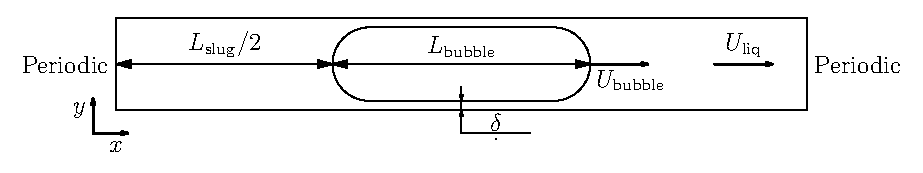
\includegraphics[width=\textwidth]{Figures/benchmark_hydro.eps}
\caption{Simplified sketch of the bubble train motion. Using periodic conditions for the velocity
field is natural, but needs validation for the mass transfer. \label{fig:benchmark:hydro}}
\end{figure}


The comparison of volumetric mass transfer coefficient
correlations with experimental correlations and establishing the Sherwood number as a function of
other non-dimensional parameters is the goal of the future work. However, as an example we will
show that one of the most recent correlations for the volumetric mass transfer coefficient by
\citet{yue-mass} resembles current simulations.

We chose to simulate mass transfer of the bubble train due to different reasons:
\begin{description}
\item[I] The gas holdup, i.e. the ratio of volume occupied by bubble to unit cell volume, is
non-negligible. Therefore, one cannot assume that the mass source is a point source which accounts
to the homogenous advection-diffusion equation with the mass source.  Therefore, there is a logical
mismatch: on one hand one needs to account the complicated geometry of the bubble and account for
all velocity pattern details, on the other hand one needs to mimic the continous picture which is
seen in experiments. One of the goals of this work is to establish certain criteria as how to
simulate such problems numerically with the help of the lattice Boltzmann method.
\item[II] For small capillary numbers as $Ca<0.7$ \cite{giavedoni-numerical} there is a vortex in
the reference frame moving with
the bubble, which  influences and improves the corresponding mass transfer.  For larger capillary
numbers there is no vortex and stremalines go around the bubble, see Fig.
\ref{fig:streamlines:tweaked:velocity}. Thus, the problem is interesting because of different
hydrodynamic patterns depending on the capillary number which governs a number of experimental
parameters as the slug length, the film thickness and the existence of the vortex in front of the
bubble. There are some available
correlations in literature \cite{bercic-mass,kreutzer-overview}. One of the particular goal of
this work is to study mass transfer dependence on the completely different velocity patterns
depending on the capillary number $Ca$. 
\end{description}
 
The numerical approach we take is the lattice Boltzmann method, a relatively new CFD
competitor emerged during last $20$ years \cite{frisch,mcnamara,HJ,HSB}. During years the
method was applied to simulate not only hydrodynamic problems \cite{yu}, but as well multiphase
flows \cite{Shan-chen:extended,swift,gunstensen}, heat transfer
\cite{yuan-thermal,zhang-thermal}, ferrofluids \cite{dellar-ferro,kuzmin-aniso}.

The mass transfer problems in the lattice Boltzmann framework were mainly addressed in series of
works of Dr. Ginzburg and co-authors
\cite{ginzburg-main,ginzburg-boundary-conditions,ginzburg-saturated-flow}. However, all these works
are of general nature to simulate the advection-diffusion equation via the lattice Boltzmann
framework. In comparison, this work aims to establish the procedure of how to obtain the
volumetric mass transfer coefficients for bubble train flow. One should mention the work of
\citet{inamuro-scalar-boundary} simulates heat and mass transfers in the porous media and the work
of \citet{jos-mass} simulates lateral mixing in cross-channel flow. While two last works are focused
at the particular mass transfer problems, both problems are of homogenuous nature and do not
guide as how to simulate the non-homogenous problems.           

The overall goal of this paper is to address the questions arised and to establish the numerical
procedure suitable to measure the volumetric mass transfer coefficient in the context of the
lattice Boltzmann method. We will utilize the results of numerical simulations of bubble flow
obtained
before \cite{kuzmin-binary2d,kuzmin-binary3d}. 

The paper is organized as follows. The mass transfer coefficients and volumetric mass transfer
coefficients definitions are covered. The limiting cases from the continuos representation and their
application to present simulations are given. The mass transfer simulations benchmarks are
presented. Finally, numerical simulations of different boundary conditions and large scale
simulations and comparison between them are presented. 

\section{Mass transfer definitions}
By the definition the mass transfer coefficient from the surface with the imposed constant
concentration $\cbubble$ is the following:
\beq
\label{eq:main:definition}
k_L=\frac{\dot{m}}{P \Delta C},
\feq
where $\dot{m}$ is the mass rate $\Bigl[\frac{kg}{s}\Bigr]$, $P$ is the area of the surface
$\Bigl[m^2\Bigr]$, $\Delta C$ is the concentration difference between the surface and the surrounding medium
$\Bigl[\frac{kg}{m^3}\Bigr]$. Therefore, $k_L$ has a dimension of velocity
$\Bigl[\frac{m}{s}\Bigr]$. Usually, the surrounding medium concentration is taken at the infinite distance
from the bubble. However, in the case of complicated geometries and non-homogeneous concentrations, 
the medium concentration can be the average concentration in the domain, the flux averaged
concentration at the inlet or outlet. Thus, one needs to establish a thorough definition of the volumetric
mass transfer coefficient in the case of complex geometries and non-trivial hydrodynamic velocity patterns.

There are different methods to estimate the mass transfer coefficient $k_L$. We first examine the
theoretical definitions of the mass transfer in case of point mass sources.
\subsection{Point mass sources}
In what follows we will present three approaches to calculate point mass transfer
coefficients:
\begin{enumerate}
\item
Let us look at the infinitesimal small domain of the volume $A \Delta x$ not
moving and with the point mass source. Then the concentration difference can be found as $\Delta C =
\cstar -
C(t)$, where $\cstar$ is the imposed point source concentration, $C(t)$ is
the time dependent average concentration. Therefore one can write the time dependent ODE for the
average concentration in the domain:
\beq
\dot{m}= A \Delta x \frac{\mathrm{d}C}{\mathrm{d} t} = k_L P (\cstar-C(t)), 
\feq
with the initial condition $C(0)=0$
The solution can be found by solving ODE:
\beq
C(t)= \cstar (1-\exp(-\vol t )), 
\feq
where $\vol$ is the volumetric mass transfer coefficient defined as:
\beq
\vol=k_L \frac{P}{V},
\feq
where $P$ is the source surface, $V$ is the unit cell volume.
\item
The previous consideration is able to predict mass transfer happening in moving with the velocity
$U$ liquid, see Fig. \ref{fig:moving:frame}. 
\begin{figure}[htb!]
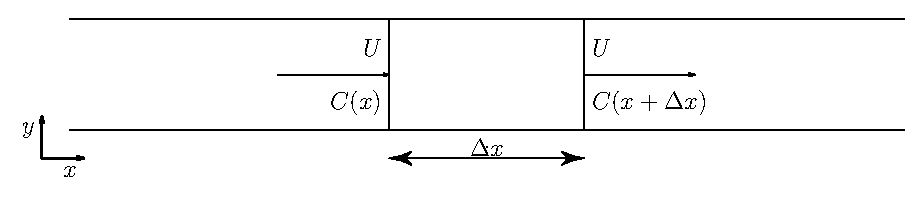
\includegraphics[width=\textwidth]{Figures/mass_transfer.eps}
\caption{The mass transfer in the moving liquid. \label{fig:moving:frame}}
\end{figure}

If one can assume that the mass point sources are distributed in the whole medium, then the mass accumulated in the unit volume $V=A \Delta x$ can be calculated as the difference of 
mass fluxes entering and leaving domain $U \bigl(C(x+\Delta x)-C(x)\bigr)$. We assume that the
source is a point source with the effective perimeter (area) $P$. The accumulated mass should be proportional
to the mass transfer coefficient:
\beq
U \bigl(C(x+\Delta x)-C(x)\bigr)=k_L P \bigl(\cstar-C(x)\bigr), 
\feq 
giving the same equation but only in the coordinate domain:
\beq
%\label{concentration:domain:coordinate}
C(x)= \cstar \Bigl(1-\exp\bigl(-k_L a \frac{x}{U} \bigr)\Bigr).
\label{main:mass:transfer:expression} 
\feq

\item If one transfers to the frame moving with the liquid velocity $U$, then the situation will be
the same as in the first case. However, one can connect the time and spatial location with the
velocity $U$ ($t=\frac{x}{U}$) to obtain the same equation as in the case 2.
\end{enumerate}

\subsection{Bubble train}
In the application to the bubble train flow, if one can think of one bubble to be a point source,
then all considerations above are valid. For example, the expression
(\ref{main:mass:transfer:expression}) was used in the experiments by
\citet{bercic-mass}. However, one should be accurate with the definition of velocities because two
different phases co-exist in the bubble train flow. Usually, one can take the velocity $U$ to be as
a bulk velocity or $U=\ugas+\uliq$, where $\ugas$ and $\uliq$ are liquid and gas
superficial velocities correspondingly. 

Though the experimental measurements are straightforward as measuring concentrations at different
locations and calculating the volumetric mass transfer coefficient through the logarithmic
function. However, if one wants to analytically estimate the mass transfer coefficients, the
situation is much more complicated because of two phases presence and complicated bubble
geometry. Phases can have different mixing patterns
from film to slug and from slug to film. As it was mentioned before depending on the capillary
number the mixing velocity pattern is different. Analytical approaches
\cite{irandoust,vanbaten-circular} assume that the
contributions from film and bubble caps can be calculated separately. However, one can see that
such 
an assumption for bubble caps (slug well mixed and the concentration is uniformly distributed over
the slug) usually overpredicts the mass transfer \cite{irandoust}. This happens since some tracer
concentration from film is mixed with the slug and changes the overall concentration in the slug.
Thus, all estimations for the analytical mass as well do not account mutual mass transfer from
neighbouring bubbles.

Another issue is that if the slug is long enough then the film saturates with the tracer
concentration and its influence on the mass transfer can be negligible \cite{vanbaten-circular}.
Mixing patterns of the film and the liquid slugs are of great importance for the analytical
estimation of the mass transfer \cite{yue-mass}. However, the assumptions usually taken for the
mass transfer calculation are small capillary number and certain mixing patterns which help to
estimate the mass transfer using the penetration theory of \citet{higbie}.

The numerical approach can take into the account the complicated mixing patterns and geometries.
However, there is a  challenge to restore the continous approach as it is seen in experiments. Next
section gives more details about numerical simulations.
 
\subsection{Numerical simulations}
\label{section:cases}
To restore the continuous picture one needs to perform a number of bubbles simulations. As we saw
before there are two approaches towards it - either to simulate
the bubble train and then to measure concentration along the pipe, Eq.
\ref{main:mass:transfer:expression}, or to transfer to the reference frame moving with the bulk
velocity $U$ and conduct same measurements. However, both methods do require a tracking of
moving bubbles which is complicated from the numerical point of view. Therefore, one needs to come
up with the simple smaller domain calculations of the mass transfer coefficient, which mimic the
continuous picture with infinite numbers of the bubbles closely. 

To avoid complications with moving grids, our
approach is to simulate mass transfer in the reference frame moving with the bubble. Therefore, one
needs to examine the equation for the continuous approach, Eq.
\ref{main:mass:transfer:expression}. 

We perform simulations in the frame moving with the bubble (velocity
$\ububble$), that the bubble position stands steady. The bubble velocity $\ububble$ is
different from the bulk velocity $\ugas+\uliq$. In this case we need to perform a coordinate $x$
variable change:
\beqal
\label{theor:average:concentration:time}
&x(t)=\ububble t\\
&C(x)=\cstar \Bigl(1-\exp\bigl(-\vol \frac{x}{\ugas+\uliq}\bigr)\Bigr)\\
&C(t)=\cstar \Bigl(1-\exp\bigl(-\vol\, t \frac{\ububble}{\ugas+\uliq}\bigr)\Bigr).
\feqal
Therefore, one can obtain the volumetric mass transfer coefficient through the concentration:
\beqal
\label{theor:one:concentration:time}
&\vol\, t \frac{\ububble}{\ugas+\uliq}=\ln \frac{\cstar}{\cstar-C(t)}\\
&\volnondim=\frac{\lunit}{\ububble t}\ln \frac{\cstar}{\cstar-C(t)},
\feqal
where the parameter $\vol \frac{\lunit}{\ugas+\uliq}$ is non-dimensional. One can also measure the
volumetric mass transfer coefficient from concentrations given at times $t_1$ and $t_2$:
\beq
\label{theor:continuous:mass:transfer}
\volnondim=\frac{\lunit}{\ububble
(t_2-t_1)}\ln\frac{C^{*}-C(t_1)}{C^{*}-C(t_2)}.
\feq
Expressions (\ref{theor:average:concentration:time}) and (\ref{theor:continuous:mass:transfer}) are
the cornerstones of the present work. The main questions arisen in the present work are to define
$C(t)$ and  the boundary conditions to produce a proper volumetric mass transfer coefficient
$\vol$. 
  
Three possible scenarios of conducting numerical simulations are possible: 
\begin{enumerate}
\item As far as the hydrodynamic flow is periodic, one can make an assumption of the same boundary
conditions applied to the tracer concentration. Therefore, only one unit cell is simulated with
periodic boundary conditions, see Fig. \ref{fig:benchmark}. As well, no tracer leaves a
domain. The situation resembles a situation for the plug flow, where no tracer can leave a unit
domain. We expect such a situation happening for small Capillary numbers $Ca<0.1$, where the film
is thin and saturates fast with the tracer. Though easier to implement, it rises certain critisism
towards the inlet concentration to be equal to the outlet concentration. In the continuous
formulation there is the concentration difference between inlet and outlet involving the volumetric
mass transfer coefficient:
\beq
\volnondim=\ln\frac{\cstar-\cinlet}{\cstar-\coutlet}.
\feq
The concentration $C(t)$ required for calculation the volumetric mass transfer coefficient, Eq.
\ref{theor:one:concentration:time}, can be taken as the average concentration in the domain:
\beq
\label{average:concentration:definition}
C(t)=\frac{\int_{liquid}{C \mathrm{d}V}}{\int{\mathrm{d}V}}.
\feq
\begin{figure}[htb!]
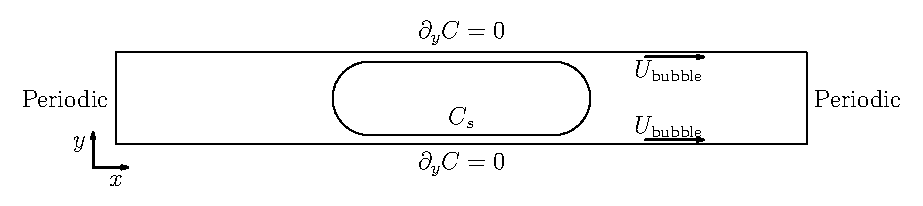
\includegraphics[width=\textwidth]{Figures/benchmark_middle.eps}\\
\caption{The two-dimensional benchmarks for the  the mass transfer
coefficient (bottom) for the bubble located near the entrance (top) and at the middle of the domain
(bottom). \label{fig:benchmark}}
\end{figure}
\item The second approach is the same as the first one but the concentration is taken as in
\cite{vanbaten-circular}. The characteristic concentration is taken as the inlet/outlet
concentration:
\beqal
&\cinlet=\frac{\int{U(y) C(0,y,t) \mathrm{d}y}}{\int{U(0,y) \mathrm{d}y}}\\
&\coutlet=\frac{\int{U(y) C(\lunit,y,t) \mathrm{d}y}}{\int{U(\lunit,y) \mathrm{d}y}}\\
&\cinlet=\coutlet.
\feqal
Therefore the assumptions  of this approach is that the difference between inlet and outlet is not
considerably large and the tracer is well mixed in the slug. 

\item
The approach of \citet{vanbaten-circular} is taken. Periodic boundary conditions were used. By the
definition the mass transfer coefficient is
proportional to the gain of the mass in the system divided by the concentration difference
multiplied on the surface area:
\beq
\vol=\frac{\dot{m}}{P \Delta C}\frac{P}{V}=\frac{\dot{m}}{V (\cstar-C(t))},
\feq
where mass difference in the domain can be calculated as:
\beq
\dot{m}=\frac{m_2-m_1}{t_2-t_1}=\frac{\int_{liq}{C(t_2)\mathrm{d}V}-\int_{liq}{C(t_1)\mathrm{d}V}}{
t_2-t_1 } .
\feq
In the approach of \citet{vanbaten-circular} the inlet and outlet concentrations were taken as the
characteristic concentration $C(t)$.

%\item 
%The approach of the opened boundaries was examined, see Fig. \ref{fig:benchmark:jos}. At the inlet
%and outlet boundaries the diffusion flux was imposed to be zero, $\frac{\partial C}{\partial x}=0$.
%The characteristic concentration was taken as the average concentration in the whole domain.
%\begin{figure}
%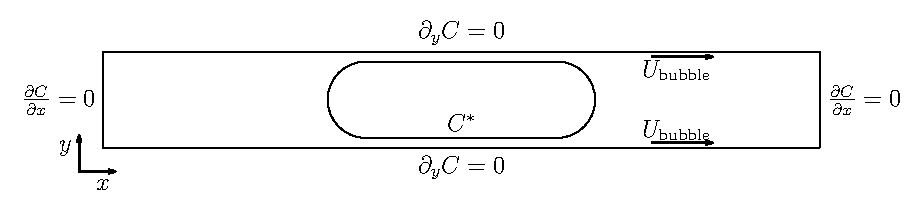
\includegraphics[width=\textwidth]{Figures/benchmark_jos.eps}
%\caption{The numerical mass transfer benchmark with open boundaries. The mass transfer is
%calculated according to Eq. \ref{theor:average:concentration:time} with the characteristic
%concentration accoring to Eq. \ref{average:concentration:definition}. \label{fig:benchmark:jos}}
%\end{figure}

\item 
The last approach to be examined in this paper is the approach of the simulation of a lot of unit
volumes, see Fig. \ref{fig:benchmark:alot}. This situation corresponds to the simulation of the
bubble train head, after injecting to the pipe and travelling along the pipe. The argument here is
that behind a certain number of the bubble train head, the influence of the boundaries will be
diminished. Thus, the average concentration in time will be governed by Eq.
\ref{theor:continuous:mass:transfer}. This simulation statement is of most correspondence to
experiments and should give right answer. However, one of the
disadvantages is to simulate a certain number of unit cells, thus increasing a computational
complexity.
\begin{figure}[htb!]
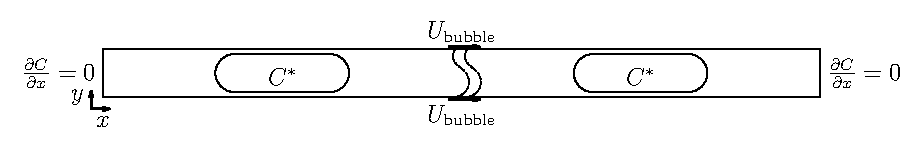
\includegraphics[width=\textwidth]{Figures/benchmark_alot.eps}\\
\caption{Benchmark for a lot of units. \label{fig:benchmark:alot}}
\end{figure}
\end{enumerate} 

Before all the approaches will be examined we will perform benchmarks of parts of geometries that
form a problem.

\section{Validation}
As for analytical expressions the problem of the mass transfer can be decomposed to the following
parts: the mass transfer from two hemispheres and the mass transfer from the film. We will examine
these problems with the help of the lattice Boltzmann method and compare them against analytical
solutions. The next sections will present the lattice Boltzmann method and a few benchmarks.

\subsection{TRT $D2Q9$ model}
The lattice Boltzmann equation (LBE) operates on a rectangular grid representing the
physical domain. It utilizes
probability distribution functions (also known as particle populations)
containing information about
macroscopic variables, such as fluid density and momentum. LBE consists of
two parts: a local collision step, and a propagation step which transports
information from one node to another along some 
directions specified by the discrete velocity set.
The LBE is typically implemented as follows:
\begin{equation}
\label{standard:implementation}
\begin{aligned}
&f_i^{*}(\bm{x},t)= f_i(\bm{x},t)-\omega \bigl(f_i(\bm{x},t)-f_i^{eq}(\bm{x},t)\bigr),&&\text{
collision step}\\
&f_i(\bm{x}+\bm{c_i},t+1)=f_i^{*}(\bm{x},t),&&\text{ propagation step}, 
\end{aligned}
\end{equation}
where $f_i$ is the probability distribution function in the direction $\bm{c_i}$,
 $f_i^{eq}$ is the equilibrium probability distribution function, $\omega$ is the
relaxation parameter. Collision operator, $-\omega \bigl(f_i- f_i^{eq}\bigr)$ is so-called BGK
collision operator \cite{bgk}. However, the approach to be used here is the TRT
(two-relaxation-times) collision operator \cite{ginzburg-main,ginzburg-saturated-flow}. In
comparison with the widely used BGK collision operator, TRT collision operator have better accuracy
for diffusion and convection fluxes, larger range of parameters where the LBM scheme is stable.

The TRT collision operator \cite{ginzburg-boundary-main}
decomposes the populations and the equilibrium
distribution into the symmetric and antisymmetric parts:
\begin{equation}
\label{trtdecomp}
f^{\pm}_i=\frac{f_i\pm f_{\bar{i}}}{2}\;,\; 
{eq_i}^{\pm}=\frac{eq_i\pm eq_{\bar{i}}}{2}\;,
\end{equation}
where $\bar{i}$ is the opposite direction to the $i$-th direction.
The collision is performed with two independent relaxation rates for 
symmetric and antisymmetric modes:
\begin{equation}
\label{trt}
\begin{aligned}
&f_i^{*}(\bm{x},t)=f_i(\bm{x},t)-\omegaplus (f_i^{+} - eq_i^+)-\omegaminus
(f_i^{-} -
eq_i^-)\\
&f_i(\bm{x}+\bm{c_i},t+1)=f_i^{*}(\bm{x},t).
\end{aligned}
\end{equation}
Note that the BGK collision operator is the particular subclass of the TRT relaxation operator with
$\omegaplus=\omegaminus$. In comparison with the BGK collision operator,
the TRT collision operator has the additional degree of freedom. Thus, the TRT operator then
introduces
so-called magic (free) parameter
$\Lambda=\Bigl(\frac{1}{\omegaplus}-\frac{1}{2}\Bigr)\Bigl(\frac{1}{\omegaminus}-\frac{1}{2}
\Bigr)$. 
This free parameter controls the effective location of the bounce-back
walls \cite{ginzburg-multireflection}, second-order accuracy of
boundary \cite{ginzburg-boundary-main} and interface schemes \cite{ginzburg-discontinious}, 
spatial accuracy \cite{ginzburg-recurrence,servan-trt-stability},
consistency \cite{ginzburg-brinkman} and, to some extent,
stability \cite{kuzmin-stability-optimal,kuzmin-d1q3,servan-trt-stability}.
In particular, $\Lambda=\frac{1}{4}$ achieves the optimal stability for the
linear advection-diffusion isotropic equation \cite{kuzmin-stability-optimal}. 

The parameters $\omegaplus$, $\omegaminus$ and $f_i^{eq}$ fully define the lattice Boltzmann
procedure. The two-dimensional nine velocities LBM $D2Q9$ is defined on the set of lattice
velocities with coordinates:
\beqal
&c_{ix}=\{0,1,0,-1,0,1,-1,-1,1\},\text{ for } i=0\dots8\\
&c_{iy}=\{0,0,1,0,-1,1,1,-1,-1\},\text{ for } i=0\dots8\,.
\feqal

The equilibrium functions for $D2Q9$ TRT model are represented as \cite{kuzmin-stability-optimal}:
\begin{equation}
\begin{aligned}
&eq_i^{+}=eq_i^{(m)}+g^{(u)} eq_i^{(u)}\\
&eq_i^{(m)}=t_i^{(m)} c_e+ eq_i^{(a)}\\
&eq_i^{(u)}=t_i^{(u)} \frac{u_x^2+u_y^2}{2}+\frac{u_x^2-u_y^2}{4} p_i^{(xx)}+g_{xy}^{(u)}\frac{u_x
u_y}{4} p_i^{xy}\\
&eq_i^{(a)}=\frac{D_{xx}-D_{yy}}{4} p_i^{xx}+\frac{D_{xy}}{4} p_i^{(xy)},
\end{aligned}
\end{equation}
where $D_{xx,yy,xy}$ are components of the diffusion tensor, $c_e=\frac{D_{xx}+D_{yy}}{2}$, the tensor $p_i^{(xx)}=c_{ix}^2-c_{iy}^2$, the tensor  $p_i^{(xy)}=c_{ix} c_{iy}$, the weights
$t_i^{(u,m,a)}$ can be chosen based on stability criteria. Though not the best set of weights for
stability, but the most spread set of weights, so called ``hydrodynamic`` weights, was chosen:
\begin{equation}
t_i^{(u)}=t_i^{(m)}=t_i^{(a)}=\Bigl\{0,\frac{1}{3},\frac{1}{3},\frac{1}{3},\frac{1}{3},\frac{1}{12},
\frac {1}{12},\frac{1}{12},\frac{1}{12}\Bigr\}
\end{equation}
 
It can be shown through the Chapman-Enskog procedure \cite{chapman}, that the simple update rule
with the equilibrium function presented above restores the anisotropic
advection-diffusion equation:
\beq
\partial_t C+ \partial_{\alpha} C u_{\alpha}=\partial_{\alpha\beta} K_{\alpha\beta} C,
\feq
where $K_{\alpha\beta}=\Bigl(\frac{1}{\omegaminus}-\frac{1}{2}\Bigr)D_{\alpha\beta}$
with the
following diffusion tensor:
\begin{equation}
D_{\alpha\beta}=
\begin{pmatrix}
D_{xx} + (g^{(u)}-1) u_x^2 & D_{xy}+(g_{xy}^{(u)}-1)u_x u_y\\
D_{xy} + (g_{xy}^{(u)}-1) u_x u_y& D_{yy}+(g^{(u)}-1) u_y^2 
\end{pmatrix}
\end{equation}
We want to resolve the isotropic advection-diffusion equation, $D=D_{xx}=D_{yy}$ or $K=K_{xx}=K_{yy}$, with the non-diagonal diffusion tensor components to be zero $D_{xy}=0$. In comparison with the $D2Q5$ model, with the $D2Q9$ it is
possible to cancel the numerical diffusion by the proper choice
of the equilibrium functions, i.e. $g_{xy}^{(u)}=g^{(u)}=1$.  The particular choice of parameters
used in simulations is $c_e=\frac{1}{3}$, $\Lambda=\frac{1}{4}$. Thus, the diffusion coefficient $K$
is matched through $\omegaminus$, i.e. $K=c_e
\Bigl(\frac{1}{\omegaminus}-\frac{1}{2}\Bigr)=\frac{1}{3}(\frac{1}{\omegaminus}-\frac{1}{2}\Bigr)$.
From hereon, without a loss of generality we refer to diffusion coefficient 
$K$ as $D$.  Free relaxation parameter $\omegaplus$ can be found through $\Lambda$. For particular
choice $\Lambda=\frac{1}{4}$ (the optimal stability parameter), $\omegaplus$ can be found easily as
$\omegaplus=2-\omegaminus$.  Fig. \ref{stability:d2q9} shows the stability limits for the $D2Q9$
model $c_e$ against $U^2=u_x^2+u_y^2$ for two particular choices.
\begin{figure}[htb!]
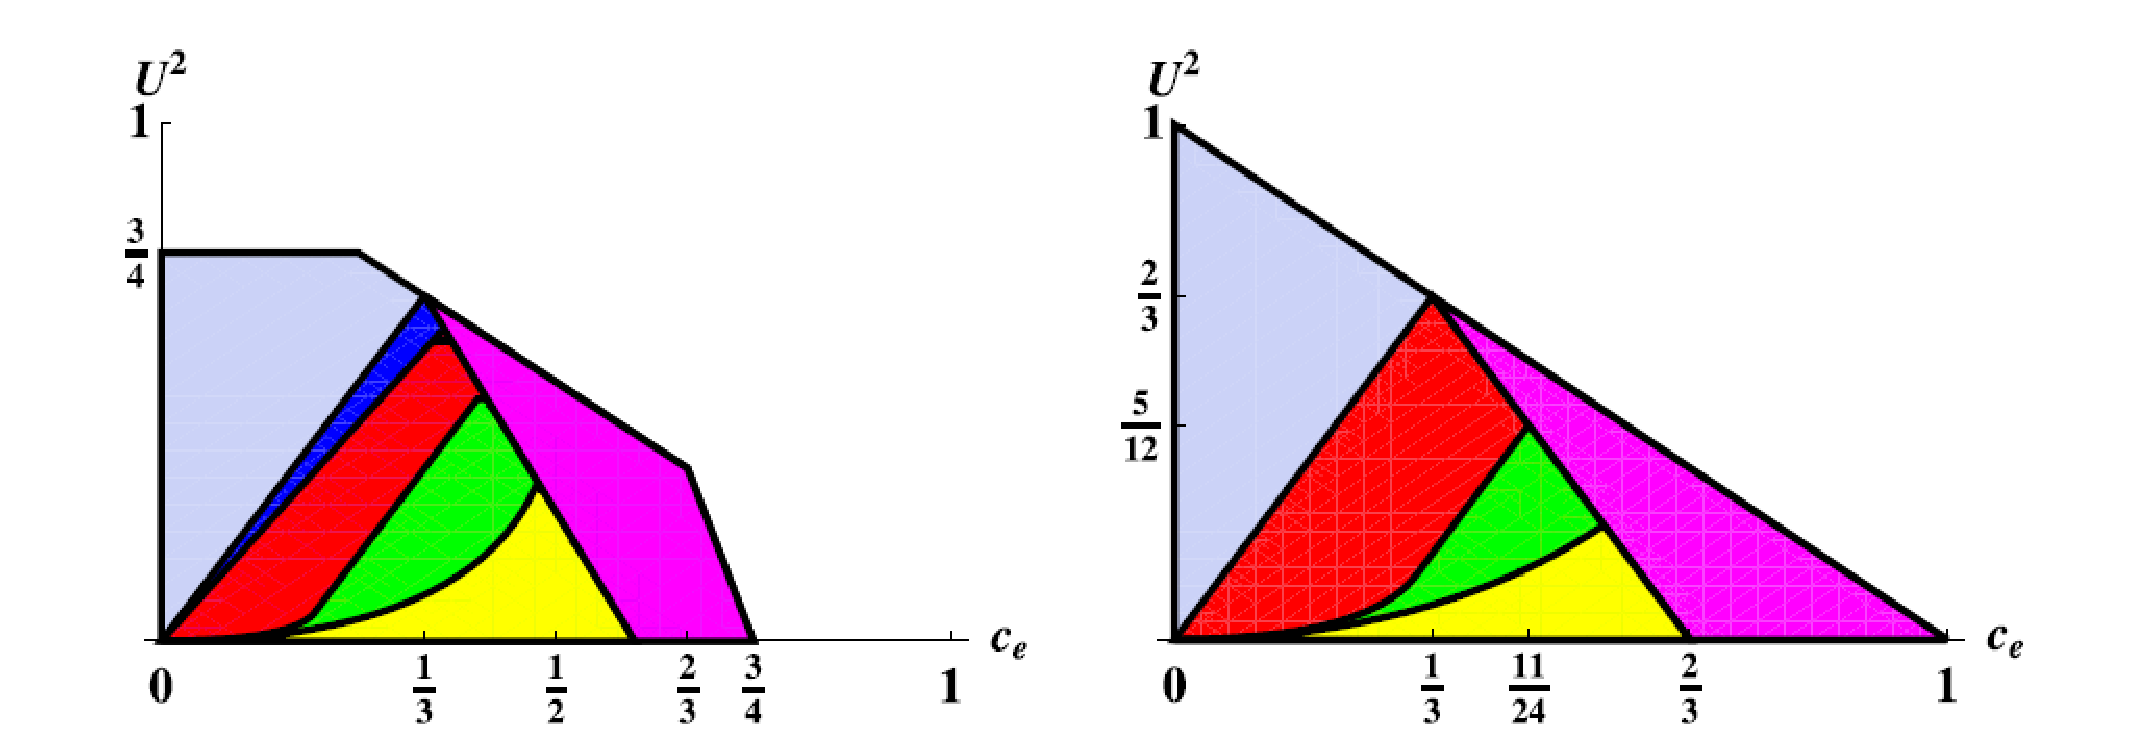
\includegraphics[width=\textwidth]{Figures/d2q9_stability.eps}
\caption{The stable sub-domains of the $D2Q9$ schemes ($\Lambda=\frac{1}{4}$)
are plotted for standard (hydrodynamic) weights (left) and uniform weights (right, not mentioned here) when the
numerical diffusion is removed, partially or completely. For particular choice used in this work (hydrodynamic weights, $c_e=\frac{1}{3}$, left picture), the achieved stable velocity is $u_x^2+u_y^2\leq\frac{2}{3}$. The non-negativity of populations (green+yellow) is for BGK stability. One can see that the achieved maximum stable velocity is twice smaller $u_x^2+u_y^2\leq \frac{1}{3}$ for the BGK collision operator.The proper choice of weights can
allow to obtain  total triangle $0 \leq u_x^2+u_y^2 \leq 1- c_e$ (the
uniform weights only).
\label{stability:d2q9}}
\end{figure}
Boundary conditions for the mass transfer used in this work are all of Dirichlet type. We validated
two types of boundary conditions: Inamuro boundary conditions \cite{inamuro-scalar-boundary} and
Pressure anti bounce-back boundary conditions \cite{ginzburg-multireflection}. However, the
simulation results presented in this work are only pressure anti bounce-back due to its simplicity
to handle any complicated type of boundary:
\beq
\label{antibb}
f^{*}_{B,i}=-f^{*}_{F,\bar{i}} + 2 eq^+(\cstar,\bm{u}),
\feq
where $\cstar$ is the concentration to be imposed at the surface, $\bm{u}$ is the surface velocity,
$i$ is the direction number pointing to the domain (unknown) located at the boundary surface $B$,
$\bar{i}$ is the direction number opposite to $i$ and is located at the fluid $F$ specifically that
$B$ is located at the location $F+c_i$. 

Note that the parameters of the lattice
Boltzmann are connected with the physical parameters only through the non-dimensional
numbers governing the physics of the problem. In our case, this number is the Peclet number, $Pe=\frac{\ububble L}{D}$.
Therefore, one can substitute any quantity, i.e.
$\ububble$ in the lattice Boltzmann units as soon as the
Peclet number is the matched in physical space and numerical simulations. This fact that $\ububble$ can be chosen arbitrarily is extremely useful in the context of numerical simulations, since can increase the time step, or decrease the computational demand by order of magnitude to obtain meaningful results. This point will be extensively covered later. 

Next section will cover LBM benchmarks for problems that form the mass transfer problem, as mass transfer from the film  and hemispheres.

\subsection{The radial case}
The case to be examined here is the mass transfer from the stair-case boundary forming a circle. It
can be
prescribed by the following system of equations:
\beq
\begin{aligned}
&\partial_t C(r,t)=\frac{1}{r}\partial_r r \partial_r C(r,t)\\
&C(a,t)=C_0,\,C(r,0)=C_{init}
\end{aligned}
\feq 
The solution is represented as \cite{chemical-correlations}:
\beq
\frac{C(r,t)-C_{0}}{C_{init}-C_{0}}=\sum_{n=1}^{\infty}{\frac{2}{\mu_n
J_1(\mu_n)}\exp\Bigl(-\mu_n^2 \frac{D t}{a^2} \Bigr)J_0(\mu_n \frac{r}{a})},
\feq
where $\mu_n$ is the $n$-th zero root of the $0$th order Bessel polynomial $J_0(\mu_n)=0$. Some of
the corresponding roots are as follows: $\mu_1=2.4048$,$\mu_2=5.5201$,$\mu_3=8.6537$,
$\mu_4=11.7915$,$\mu_5=14.9309$.
By taking initial concentration to be $0$, one can obtain the following solution:
\beq
C(r,t)=C_0 \Biggl(1 - \sum_{n=1}^{\infty}{\frac{2}{\mu_n
J_1(\mu_n)}\exp\Bigl(-\mu_n^2 \frac{D t}{a^2} \Bigr)J_0(\mu_n \frac{r}{a})}\Biggr).
\feq

The solution depends only on the non-dimensional time: $\tau=\frac{D t}{a^2}$. The domain size was $129\times 129$ with the circle radius $a=40$ units. Some examples for
different diffusion coefficients are presented in Fig.\ref{fig:cylinder:benchmark}.
\begin{figure}[htb!]
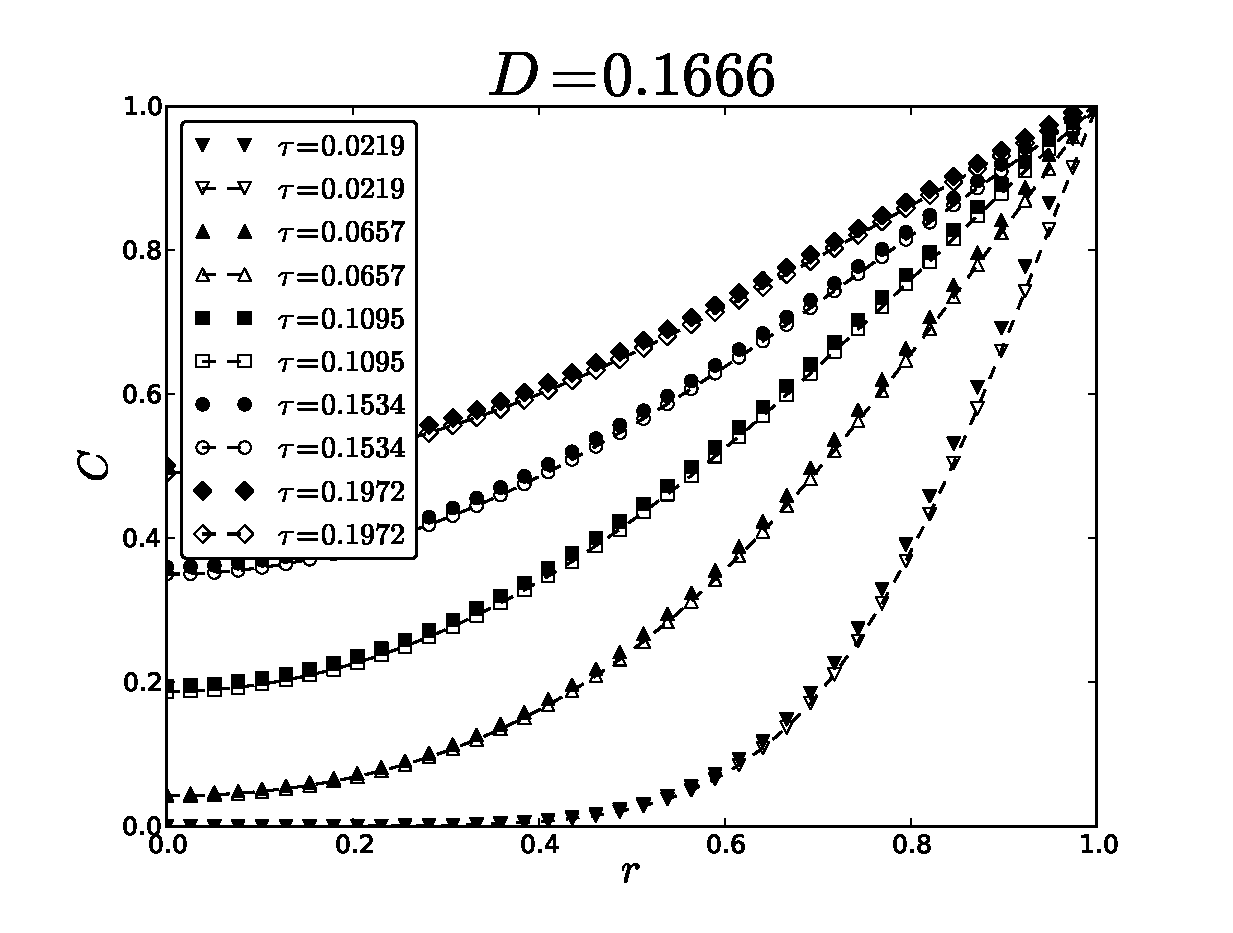
\includegraphics[width=0.5\textwidth]{Figures/cylinder1666.eps}
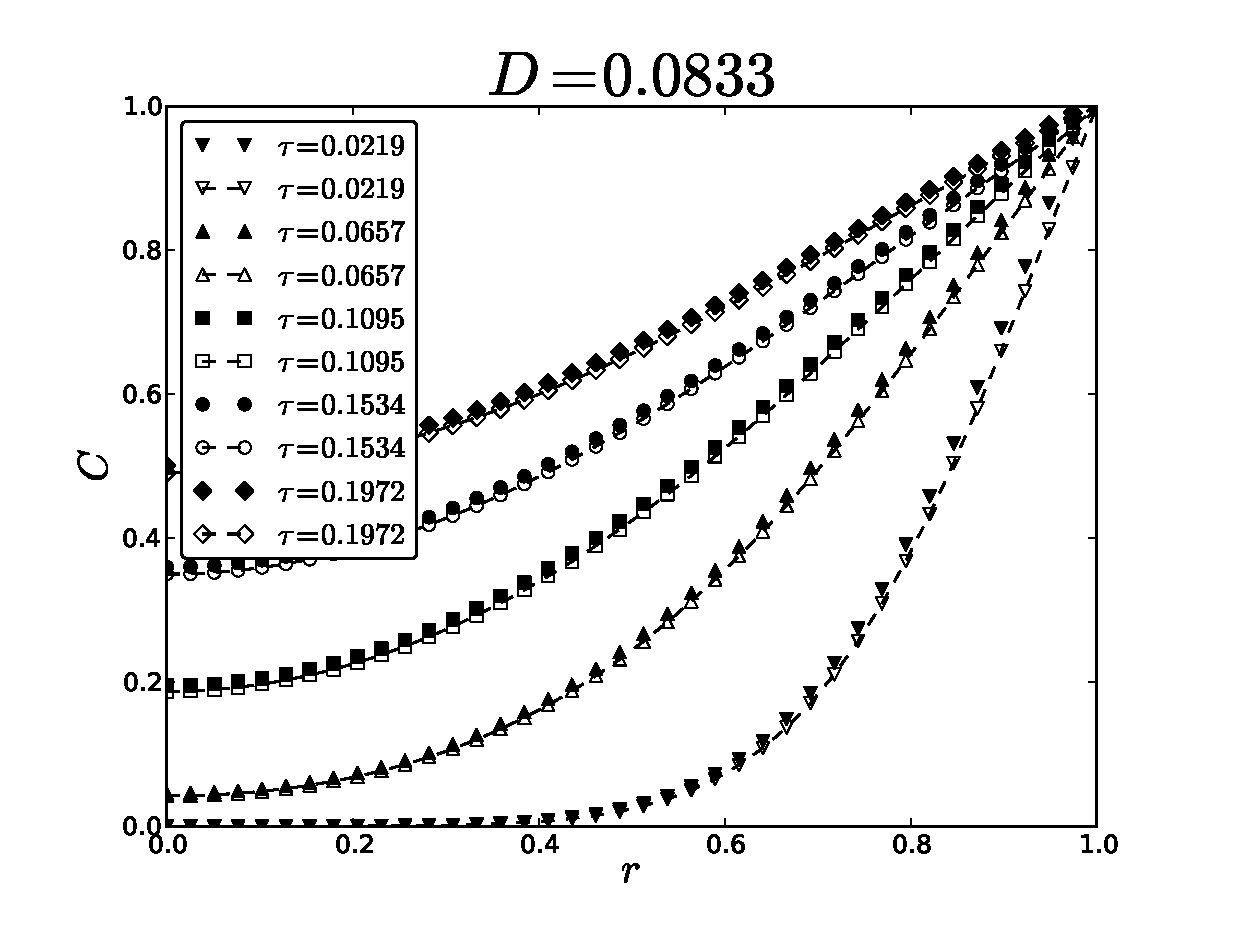
\includegraphics[width=0.5\textwidth]{Figures/cylinder0833.eps}\\
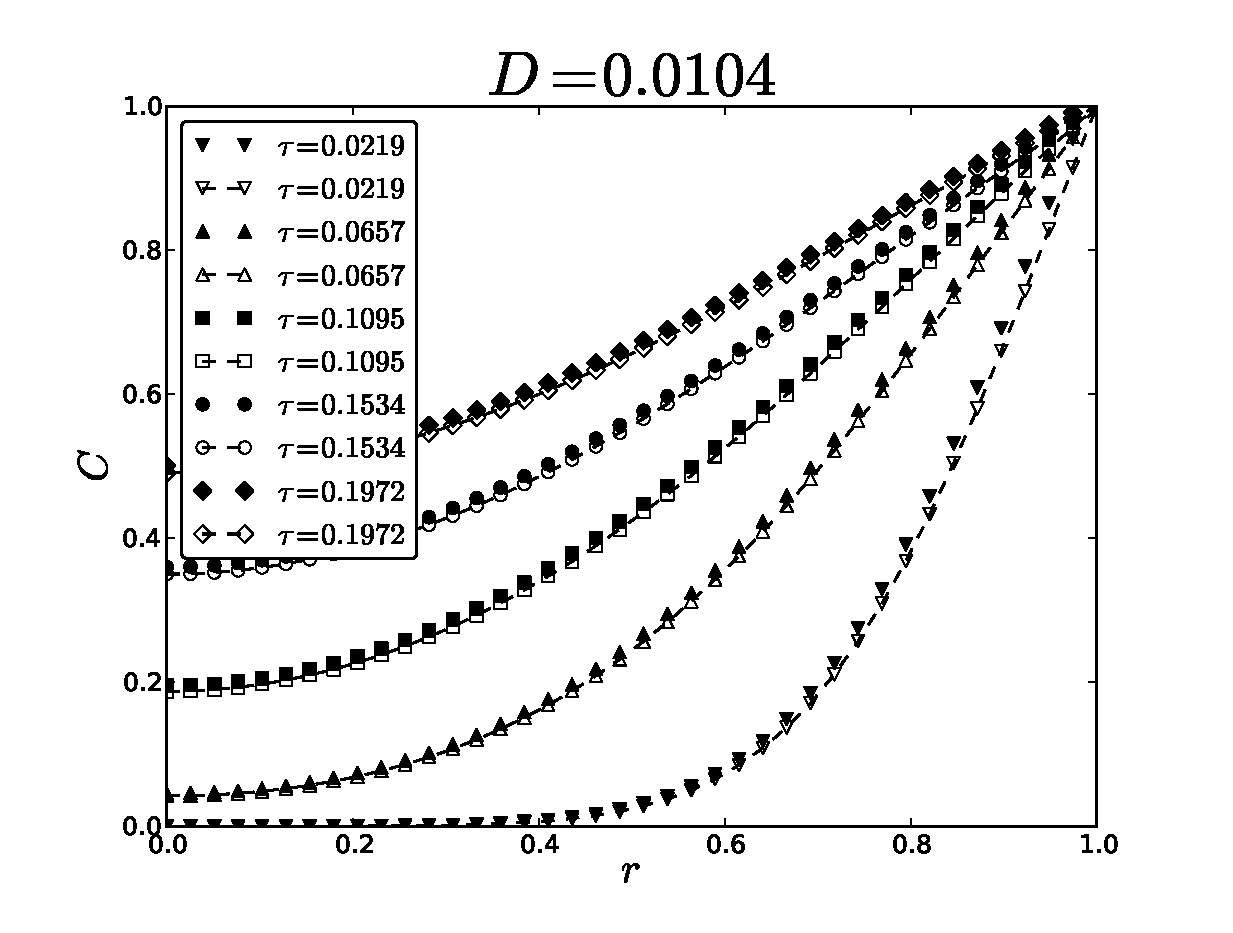
\includegraphics[width=0.5\textwidth]{Figures/cylinder0104.eps}
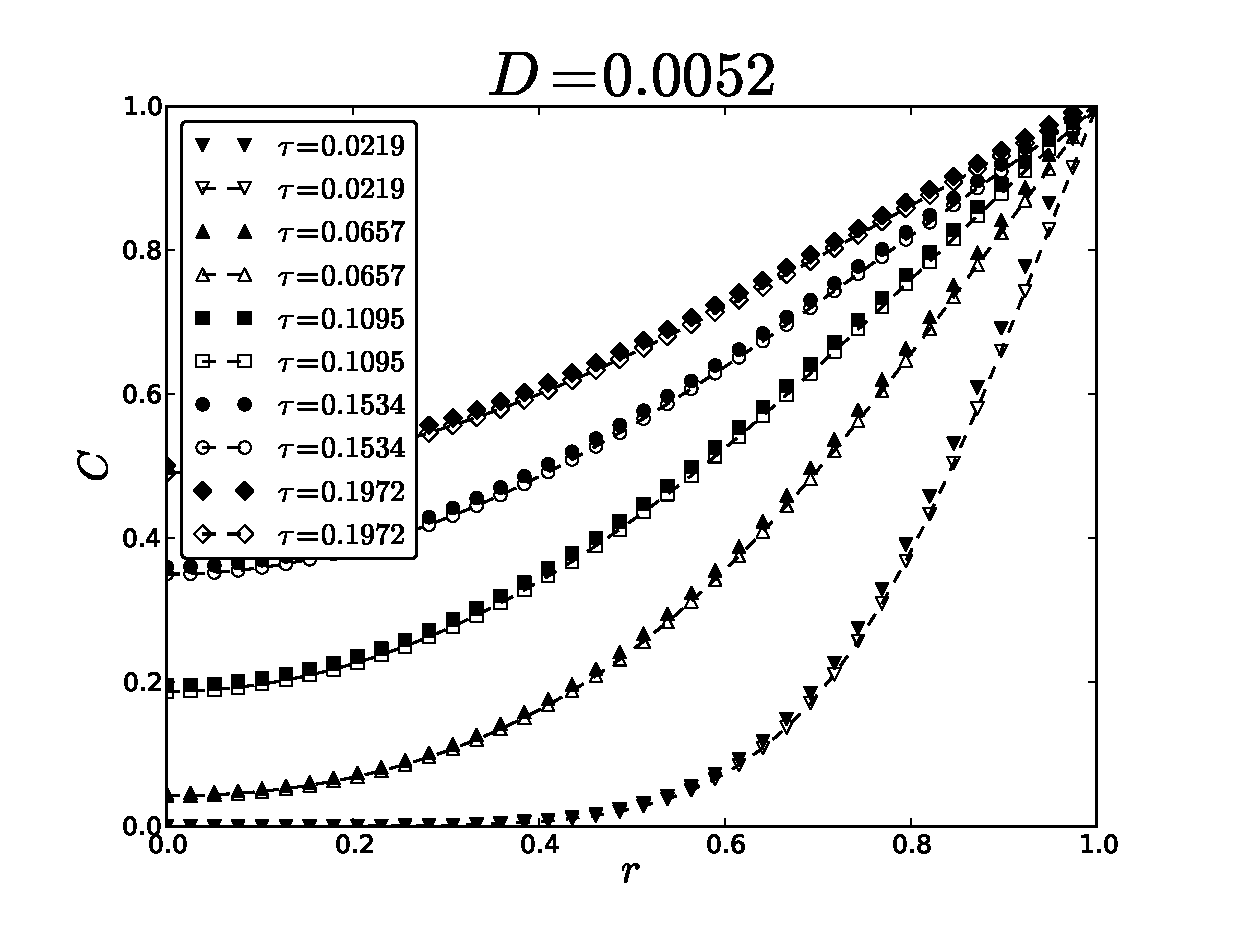
\includegraphics[width=0.5\textwidth]{Figures/cylinder0052.eps}\\
\caption{Profiles for different diffusion parameters varied with $\omegaminus$. One can see that the diffusion from the non-linear boundaries is captured
accurately \label{fig:cylinder:benchmark}.}
\end{figure}

\subsection{Parabolic profile with the velocity zero gradient at the wall}
The problem is defined in terms of PDE as follows: 
\beq
\begin{aligned}
&\frac{\partial C}{\partial x} U(y)=D\frac{\partial^2 C}{\partial y^2}\\
&C(0,y)=C_0,\, C(x,0)=\cstar,\, \frac{\partial C}{\partial y }(x,\delta)=0\\
&U(y)=U_0 \Bigl(\frac{y}{\delta}\Bigr)^2.
\end{aligned}
\feq
The procedure to solve this PDE is presented in Appendix \ref{appendix:zero:gradient}:
\beq
\label{analytical:solution:zero:gradient}
\begin{aligned}
&C(x,y)=\cstar+\sum_{m}{C_m
\sqrt{\frac{y}{H}}J_{\frac{1}{4}}\Bigl(\frac{m^2}{2}\frac{y^2}{H^2}\Bigr)\exp\Bigl(-\frac{m^4}{Pe}
\frac { x }{H}\Bigr)}\\
&C_m = (C_0-\cstar \frac{\int_{\xi=0}^{1}{\xi^{5/2} J_{\frac{1}{4}}\Bigl(\frac{m^2
\xi^2}{2}\Bigr)\mathrm{d}\xi}}{\int_{\xi=0}^{1}{\xi^3 J_{\frac{1}{4}}^2\Bigl(\frac{m^2
\xi^2}{2}\Bigr)\mathrm{d}\xi}}
\end{aligned}
\feq
Fig. \ref{fig:parabolic:zero:gradient} shows the steady-state contours comparison between the
analytical and the simulation with the Anti Bounce-Back conditions used to impose constant
concentrations at the wall $\cstar=1$ and the inlet $C_0=0$. The grid used in the simulation is
$80\times1600$. Parameter $\omegaminus=1.8$ implies the diffusion coefficient to be
$D=\frac{1}{3}\Bigl(\frac{1}{\omega}-\frac{1}{2}\Bigr)=0.0185$.  
\begin{figure}[htb!]
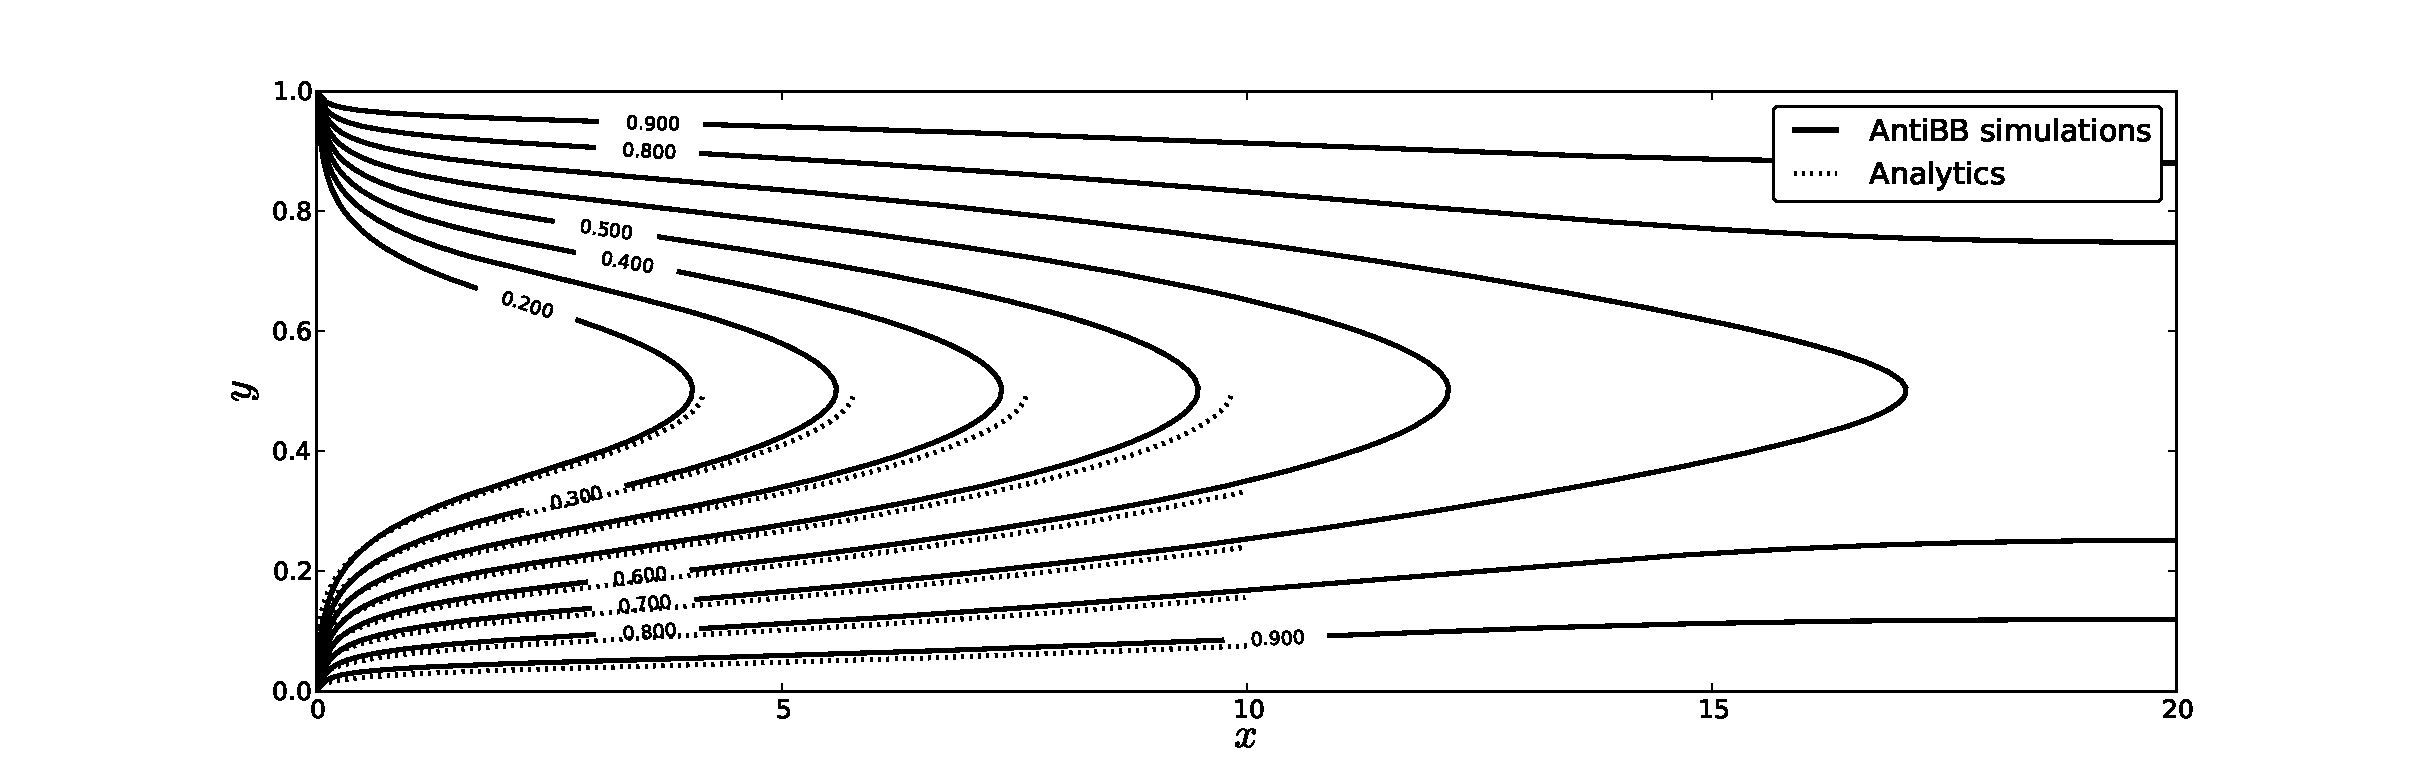
\includegraphics[width=\textwidth]{Figures/parabolic_profile_zero_gradient_comparison.eps}
\caption{Comparison with the analytical concentration contours, Eq.
\ref{analytical:solution:zero:gradient}, for the diffusion coefficient $D=0.0185$. Simulation was
performed on grid $80\times 1600$. The constant concentration is imposed with the
anti bounce-back conditions, Eq. \ref{antibb}. \label{fig:parabolic:zero:gradient}}
\end{figure}
 
\subsection{Poiseulle velocity parabolic profile}
The problem we want to address can be formulated through the following PDE:
\beq
\begin{aligned}
&\frac{\partial C}{\partial x} U(y)=D\frac{\partial^2 C}{\partial y^2}\\
&C(0,y)=0,\, C(x,\pm \delta)=\cstar,\, \frac{\partial C}{\partial y }(x,0)=0\\
&U(y)=U_0 \Bigl(1-\bigl(\frac{y}{\delta}\bigr)^2\Bigr)
\end{aligned}
\feq
The procedure to solve this problem is presented in Appendix \ref{appendix:poiseuille} which yields
the final solution as:
\begin{equation}
C=\cstar-\cstar \sum_{m=0}{C_m e^{-m^4 \frac{x}{\delta}\frac{1}{Pe}} e^{-m^2
y^2/(2\delta^2)}{_1F_1}\Bigl(-\frac{m^2}{4}+\frac{1}{4},\frac{1}{2},m^2 \frac{y^2}{\delta^2}\Bigr)},
\end{equation}
where coefficients $C_m$ are taken from Eq. \ref{coeff:series:parabolic:profile}. The comparison
between contours of analytical and simulation results is presented in Fig.
\ref{fig:parabolic:comparison}. Parameters were taken the same as in the previous case: the
diffusion $D=0.0185$, the grid dimension is $80\times1600$. 
\begin{figure}[htb!]
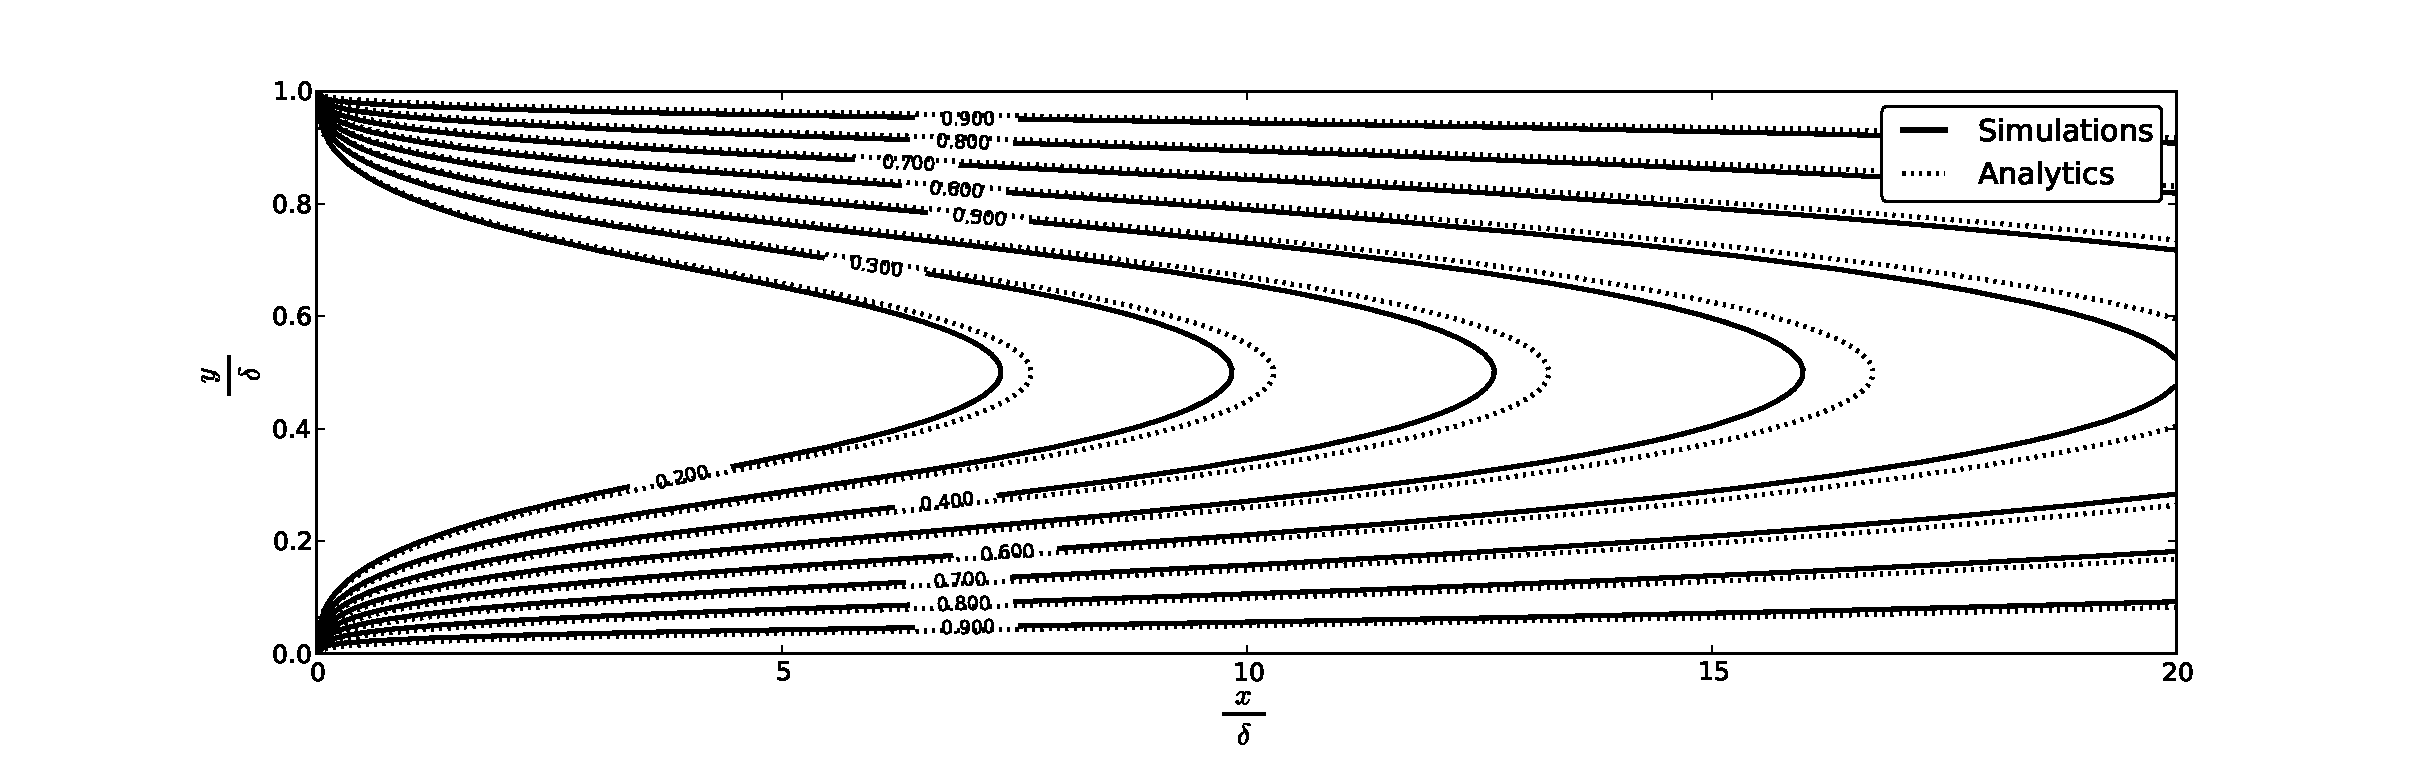
\includegraphics[width=\textwidth]{Figures/parabolic_profile_comparison.eps}
\caption{Comparison between the analytical concentration contours and simulations with pressure
anti bounce-back conditions, Eq. \ref{antibb}. The parameters were
taken as $D=0.0185$ and grid $80\times1600$. \label{fig:parabolic:comparison}}
\end{figure}

After the LBM is validated against the benchmarks relevant for the flow around bubbles, one can
examine all the cases to calculate the volumetric mass transfer coefficient, Section
\ref{section:cases}.

\section{Numerical approach}
\label{sec:numerics}
The code was utilized to obtain the flow patterns for different capillary numbers
\cite{kuzmin-binary2d}. Five particular cases were chosen to examine, their results are summarized
in Table \ref{table:capillary:cases}. 
\begin{table}[htb!]
\begin{tabularx}{\textwidth}{|X|X|X|X|X|X|X|X|X|}
\hline
$Ca$    &$Re$     &$\ububble$ &$\delta$&$\holdup$
&$\uliq$&$\ugas$&$\lbubble$&$\lslug$\\
\hline
$0.097$ &$1.656$  &$0.0055$ &$0.092$ &$0.30$ &$0.0046$&$0.0016$&$5.79$&$9.21$\\ 
$0.254$ &$4.318$  &$0.0143$ &$0.132$ &$0.28$ &$0.0108$&$0.0041$&$6.12$&$8.88$\\ 
$0.526$ &$8.938$  &$0.0297$ &$0.157$ &$0.27$ &$0.0209$&$0.0080$&$6.19$&$8.81$\\
$0.750$ &$12.744$ &$0.0424$ &$0.167$ &$0.25$ &$0.0293$&$0.0107$&$5.96$&$9.04$\\
$1.040$ &$17.665$ &$0.0588$ &$0.177$ &$0.22$ &$0.0397$&$0.0135$&$5.59$&$9.41$\\
\hline
\end{tabularx}
\caption{Sample results with the binary liquid lattice Boltzmann model \cite{kuzmin-binary2d}. The
following notations are used: the capillary number $Ca=\frac{\ububble L}{\rho \nu}$, $\delta$ is the
non-dimensional film thickness, $\uliq$ is the superficial liquid velocity, $\ugas$ is the
superficial gas velocity. One can see the sketch of the simulation in Fig.
\ref{fig:benchmark:hydro}. \label{table:capillary:cases}}
\end{table}
One can check that velocities in Table \ref{table:capillary:cases} are small. It means that to
match large Peclet numbers, $Pe=\frac{\ububble L}{D}$, usually seen in experiments to measure
the mass transfer coefficient, one needs to decrease
$D=\frac{1}{3}\Bigl(\frac{1}{\omegaminus}-\frac{1}{2}\Bigr)$. However, for parameters
$\omegaminus \approx 0.5$ the stability of the lattice Boltzmann method drastically decreases
\cite{kuzmin-d1q3}. On the other hand, one iteration in the lattice Boltzmann system corresponds
to the time in the physical domain as $\Delta t=U_{\mathrm{bubble,LB}} \frac{\Delta
x}{U_{\mathrm{bubble,phys}}}$. This time is proportional to the velocity of the $U_{\mathrm{LB}}$
and the typical number of simulation steps to obtain necessary number with given velocities for
$Ca<0.2$ is of the order of a few millions. Thus, one wants to increase the available velocity
while keeping the Peclet number the same. This helps to stability of the method as well, since
$\omegaminus$ is not close to its stability limit $\omegaminus=0.5$. 

Given all the considerations above, one needs to approach the mass transfer in the following
steps:
\begin{description}
 \item[Flow field] Given the capillary number $Ca$, one needs to obtain hydrodynamic fields around
the bubble using the binary liquid lattice Boltzmann model according to work
\cite{kuzmin-binary2d}. Periodic boundary conditions are used. The grid used in this work is
$202\times 3000$ which corresponds to fluid domain size $200\times3000$. The grid resolution is
taken to insure grid
independency of results.  
 \item[Bubble reference frame] Once the hydrodynamics is resolved, the mass transfer simulations
are conducted in the moving reference frame with the bubble. Then the bubble stands still and the
flow is coming around the
bubble. We impose a steady concentration of the trace on the surface
of the bubble with the anti bounce-back condition, Eq. \ref{antibb}.
 \item[Velocity improvement] Due to necessity to increase velocity one can scale the velocity to
perform fast simulations, one needs to improve velocity. This issue arises because of the
multiphase model used in simulations.The binary liquid lattice Boltzmann model is the diffusive
interface model. Thus, the
transition between gas and liquid is the continuous function. We obtain the bubble shape according
to the phase indicator $\phi$ as used in \cite{kuzmin-binary2d}, say $\phi<0$. The velocity of the
bubble is calculated as the bubble tip velocity. Because of the highly non-linear diffusive
interface model the shape of the bubble is determined within accuracy of one grid node, as well
there is the error in determination in the bubble velocity. Though these errors are small, however
there is small non-zero velocity component pointing to the bubble in some places, see Fig. 8 in
\cite{kuzmin-binary2d} where some streamlines are penetrating a bubble surface a bit.
This small velocity is amplified upon the velocity scaling and is inconsistent with the
advection-diffusion equation.


Thus, before performing the mass transfer simulations one additional one-component hydrodynamic
simulation is performed. A special additional free-surface solver was developed in order to dispose
the normal to surface velocity components. We take results from the multiphase simulations, extract
bubble shape using the phase indicator $\phi<0$, approximate the bubble shape by the stair-case
line. Then,the obtained bubble velocity is imposed on walls. This corresponds to conducting
simulation in the reference frame moving with the bubble. In addition, the free-slip boundary
condition on the bubble surface is imposed. Appendix \ref{appendix-free-surface} covers the simple
free-slip boundary conditions drastically improving velocity patterns. The system is tterate until a
steady state is reached. Note, that these type of simulations are much faster than original
multiphase simulations. As the output all the non-zero velocity components perpendicular to the
bubble surface are completely illuminated. We compared original multiphase simulations with
one-component free-slip simulations. All quantities as superficial slug and bubble velocities are
within $3\%$ for the capillary number in the range $0.05\leq Ca \leq 1.0$. This small trick helps to
make mass transfer simulations stable and faster, since the velocity scaling can be done easier. One
can see in Fig. \ref{fig:free:surface} two streamlines profiles for $Ca=0.097$  and $Ca=1.040$.
\begin{figure}[htb!]
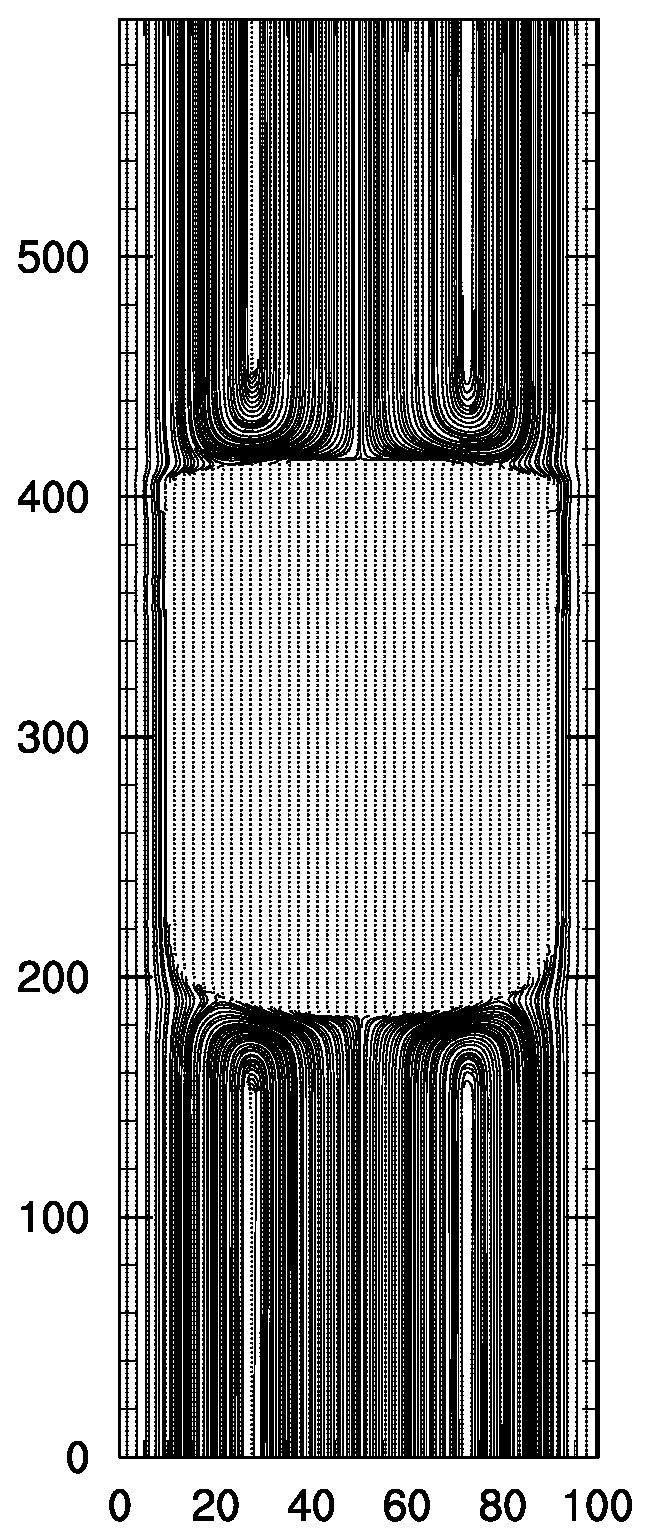
\includegraphics[angle=90,width=\textwidth]{Figures/performed_ca0097.eps}\\
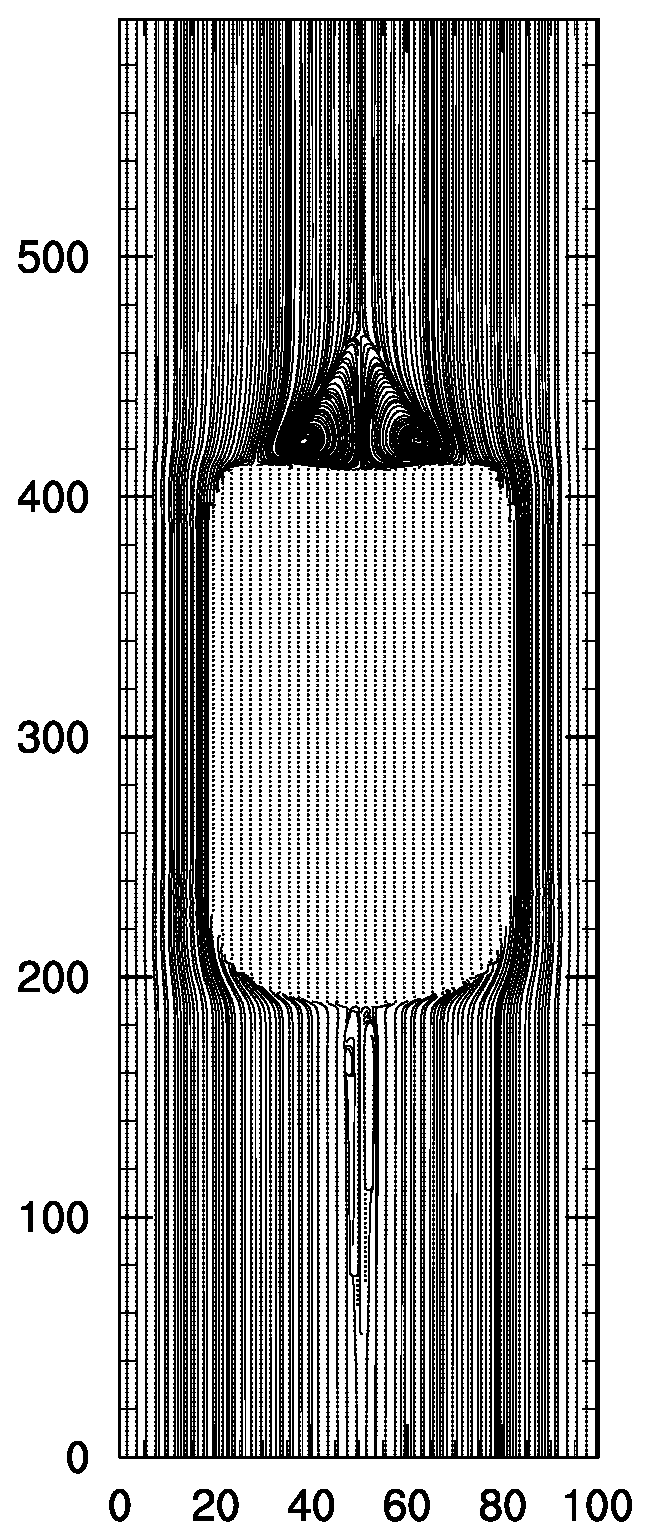
\includegraphics[angle=90,width=\textwidth]{Figures/performed_ca1040.eps}
\caption{The streamlines patterns produced by the free-surface solver with simplistic approximation
of the free-slip bubble surface, see Appendix \ref{appendix-free-surface}. Two completely different
velocity patterns are covered, $Ca=0.097$ (top) and $Ca=1.040$ (bottom).
\label{fig:streamlines:tweaked:velocity}}
\end{figure}

\item[Mass transfer] After improved velocity profiles are obtained one can perform any mass
transfer simulations with different boundary conditions as covered in Section \ref{section:cases}.
For this purpose one needs to match the Peclet number $Pe$ from experiments. Note that we
specifically separated the hydrodynamic problem from the mass transfer problem. When one wants to
solve these simultaneous problems, then one needs to match all the non-dimensional parameters, as
the capillary number (viscous forces over surface tension), the Schmidt number (viscous diffusion
rate over mass diffusion rate), the Peclet number (convection over diffusion), the Reynolds number
(inertia over viscous forces) and the Sherwood
number (convection mass transfer over diffusion mass transfer):
\begin{equation}
\begin{aligned}
&Re=\frac{\ububble L}{\nu_{\mathrm{liq}}},&&Ca=\frac{\ububble \mu_{\mathrm{liq}}}{\gamma}\\
&Pe=\frac{\ububble L}{D},&&Sh=\frac{K L}{D}\\
&Sc=\frac{\nu_{\mathrm{liq}}}{D}.&&
\end{aligned}
\end{equation}
\end{description}

\section{Results}
This section covers simulation results. We first examine the possibility to increase the fluid
velocity while keeping the Peclet number the same. After that we will examine the periodic boundary
conditions for $5$ capillary cases, open boundary simulations, and finally we will examine many
cells simulations for two representative cases velocity patterns, as $Ca=0.0907$ and $Ca=1.04$
(see Fig. \ref{fig:streamlines:tweaked:velocity}). 

\subsection{Keeping Peclet}
\label{section:keeping:peclet}
This section addresses the performance of the simulations. The ulimate goal is to increase
velocity at least by several orders while keeping dimensionless parameters the same to speed up
simulations. Increasing velocity can also help to resolve a lot of unit cells to represent a
continous picture.

With the given bubble shape and velocity pattern only nondimensional parameter Peclet number governs
the advection-diffusion equation:
\beq
Pe=\frac{\ububble N_y}{D}.
\feq
As far as we want to increase velocity, that
means one needs to increase the diffusion coefficient as well. The runs were made with
velocities $2,4,6,8,10,15,20,40$ times larger than original velocities. The velocities we chose and
its corresponding capillary numbers are presented in Table \ref{table:scaling:peclet}. Periodic
boundary conditions were used and mass transfer coefficient was calculated according to Eq.
\ref{main:simulation:equation}. Table \ref{table:scaling:peclet} shows that the velocity limit
for  periodic boundary conditions is $0.1$ where $\omegaminus=1.99$ ($D=0.000837$). It gives us the
preliminary idea to what extent one can scale periodic mass transfer simulations. 
\begin{table}[htb!]
\begin{tabularx}{\textwidth}{|X|X|X|X|}
\hline
Scale&$U_{bubble}$&Time Iterations&$C_{aver}$\\
\hline
\multicolumn{4}{c}{}\\
\multicolumn{4}{c}{$Ca=0.097$,$Pe=1313$}\\
\hline
$2$ &$0.011$&$400000$&$0.318$\\
$4$ &$0.023$&$200000$&$0.319$\\
$8$ &$0.044$&$100000$&$0.320$\\
$10$&$0.055$&$80000$ &$0.321$\\
$20$&$0.11 $&$40000$ &$0.324$\\
$40$&$0.22 $&$20000$ &$0.328$\\
\hline
\multicolumn{4}{c}{}\\
\multicolumn{4}{c}{$Ca=0.254$,$Pe=3414$}\\
\hline
$2$& $0.0286$&$800000$&$0.6533$\\
$4$& $0.0572$&$400000$&$0.6591$\\
$8$& $0.1144$&$200000$&$0.6692$\\
$10$&$0.1430$&$160000$&$0.6734$\\
$20$&$0.2860$&$80000$ &$0.6894$\\
\hline
\multicolumn{4}{c}{}\\
\multicolumn{4}{c}{$Ca=0.526$,$Pe=7092$}\\
\hline
$2$&$0.0594$&$200000$&$0.3271$\\
$4$&$0.1188$&$100000$&$0.3315$\\
\hline
\multicolumn{4}{c}{}\\
\multicolumn{4}{c}{$Ca=0.750$,$Pe=10125$}\\
\hline
$2$&$0.0848$&$200000$&$0.3489$\\
\hline
\multicolumn{4}{c}{}\\
\multicolumn{4}{c}{$Ca=1.040$,$Pe=14041$}\\
\hline
$2$&$0.1176$&$200000$&$0.3675$\\
\hline
\end{tabularx}
\caption{Table representing how one can speed up simulations. One iteration in the lattice
Boltzmann system corresponds to time difference as
$\Delta t=\frac{U_{\mathrm{bubble,LB}}}{U_{\mathrm{bubble,phys}}} \Delta x$. Therefore the speed up
of the simulation is proportional to the  $U_{\mathrm{bubble,LB}}$. Thus, the time iterations
indicated in the table correspond to the one time moment in physical space. One can see that
scaling produces adequate results.  One can see that the stability limit is approximately around
$U_{bubble}=0.1$ for the diffusion coefficient
$D=1/3(1/1.99-0.5)=0.000837$. Average concentrations are in the reasonable agreement. The contour
profiles for all of these cases are presented in Fig. \ref{fig:contours:scaling:peclet}
\label{table:scaling:peclet}}
\end{table}
The corresponding to Table \ref{table:scaling:peclet} concentration contour profiles for different
velocity scalings are presented in Fig. \ref{fig:contours:scaling:peclet}. One can see an
acceptable agreement between all of them. Note, that a few profiles are obtained $10$ to $40$ times
faster.
\begin{figure}[htb!]
\includegraphics[height=0.25\textwidth]{Figures/contourlines_scale_ca097.eps}\\
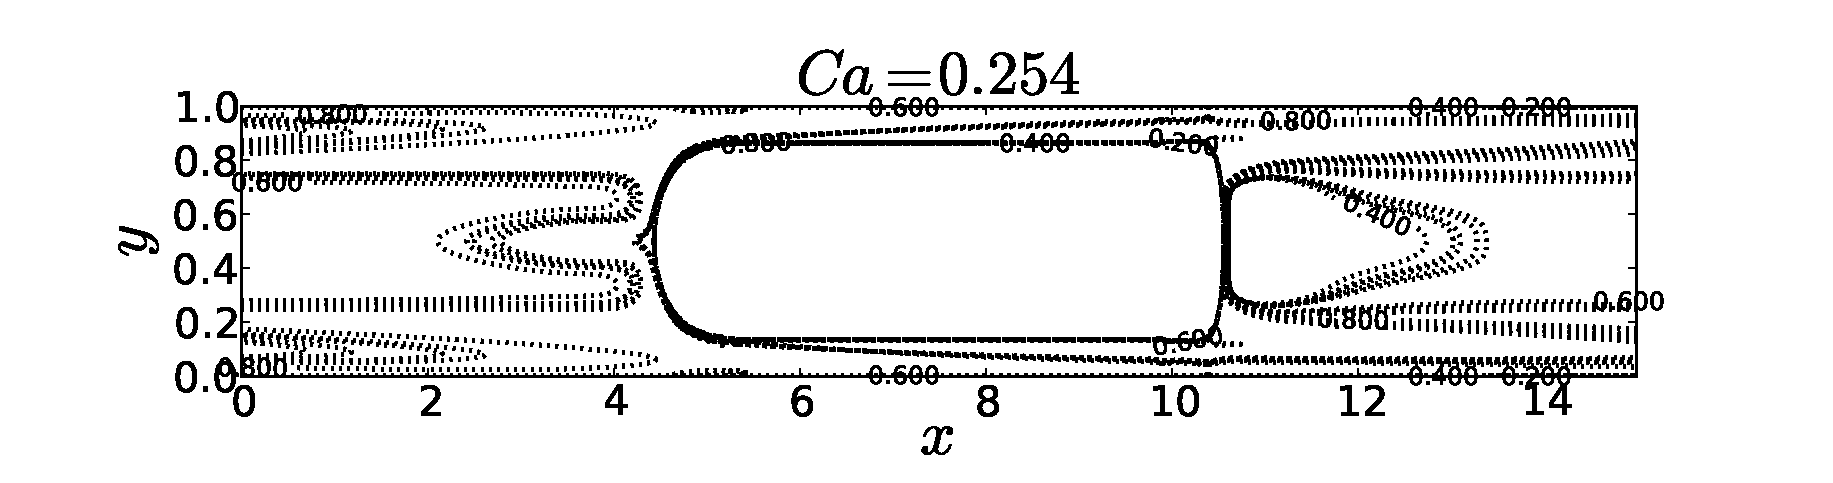
\includegraphics[height=0.25\textwidth]{Figures/contourlines_scale_ca054.eps}\\
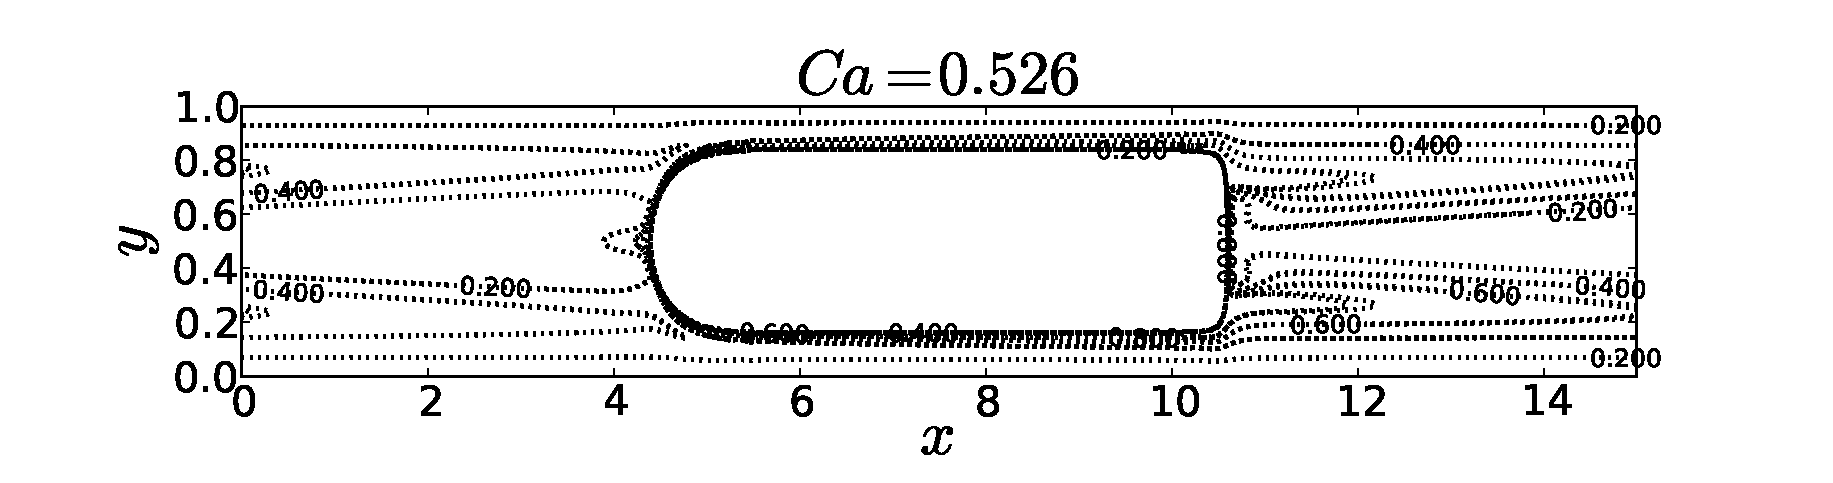
\includegraphics[height=0.25\textwidth]{Figures/contourlines_scale_ca026.eps}\\
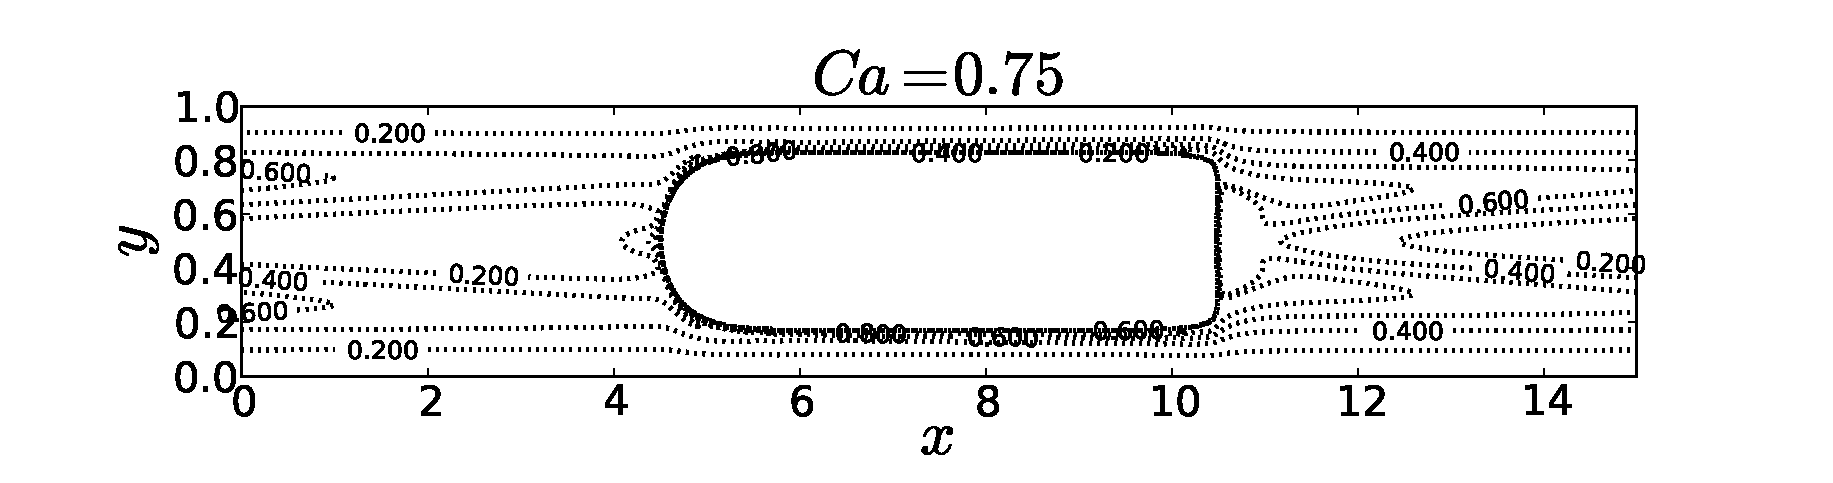
\includegraphics[height=0.25\textwidth]{Figures/contourlines_scale_ca05.eps}\\
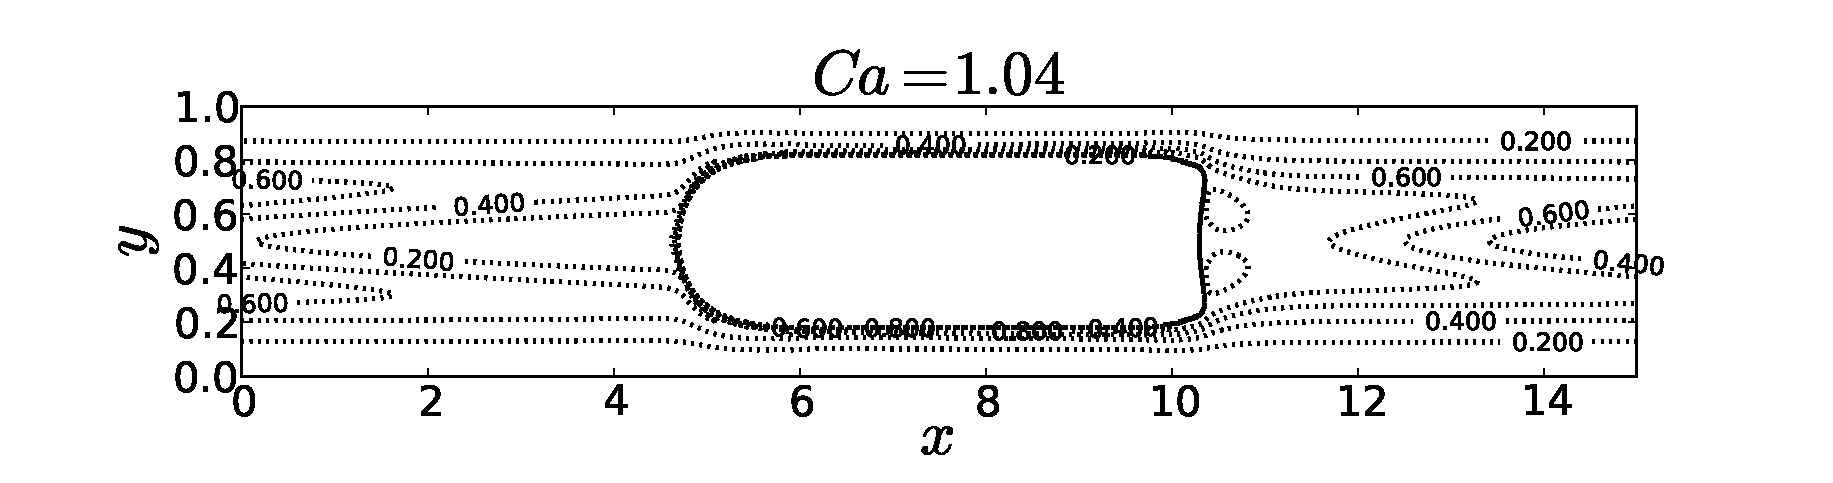
\includegraphics[height=0.25\textwidth]{Figures/contourlines_scale_ca14.eps}\\
\caption{Concentration contour profiles for velocity scalings as identified in Table
\ref{table:scaling:peclet} (top to bottom:
$Ca=0.097,0.254,0.526,0.750,1.040$).\label{fig:contours:scaling:peclet}}
\end{figure}

\subsection{Average concentration}
\label{main:results:periodic}
As indicated in Section \ref{section:cases} one can calculate the average domain concentration over
the time. Eq. \ref{theor:one:concentration:time} shows how 
the volumetric mass transfer coefficient depends on
time, i.e. streamwise coordinate:
\beqal
&\vol t \frac{\ububble}{\ugas+\uliq}=\ln\frac{\cstar}{\cstar-C(t)}\\
&\vol \frac{\lunit}{\ugas+\uliq}=\frac{\lunit}{\ububble t} \ln \frac{C^*}{C^*-C(t)},\\
\feqal
where $C(t)$ is the average concentrations.
Simulations for coefficient $\vol \frac{\ububble}{\ugas+\uliq}$ are shown in Fig.
\ref{fig:aver:conc:different:capillaries:time} for different Peclet numbers and velocity scalings
indicated in Table \ref{table:scaling:peclet}. Because in the definition of the volumetric mass
transfer coefficient there is the logarithm function, thus when the average concentration goes
close to $\cstar=1$ then Eq. \ref{theor:one:concentration:time} gives inadequate results due to
 accuracy of the logarithmic function. However, the more interesting thing is to put the same plots
as in Fig. \ref{fig:aver:conc:different:capillaries:time} against the number of unit cells length
which the bubble passes with the given velocity as $\mathrm{scale}\cdot\frac{\mathrm{\ububble\cdot
t}}{L}$. Fig. \ref{fig:aver:conc:different:capillaries} shows the volumetric mass transfer
dependency against the distance in unit cells length. One can see in Table
\ref{table:steady:state:average} that for different Peclet numbers different time (number of unit
cells) is required to achieve the steady state. Also, Table \ref{table:steady:state:average} shows
the achieved steady state volumetric mass transfer coefficient. One can see tendention that for
larger Peclet number less time steps are required to achieve the steady state condition. 

Overall one is guaranteed to obtain the steady state volumetric mass transfer coefficient for
periodic boundaries simulations if the following conditions are fulfilled:
\begin{description}
\item Scaling is performed as $U_{max}=\mathrm{scale}\cdot\ububble\leq 0.1$.
\item The larger Peclet number the less time is required. One can extrapolate data from Table
\ref{table:steady:state:average}, say $L_{\mathrm{steady}}$ and perform the following number of
iterations as $\mathrm{scale}\cdot \ububble\cdot N_{\mathrm{iter}}\leq L_{\mathrm{steady}}$. 
\end{description}

\begin{figure}[htb!]
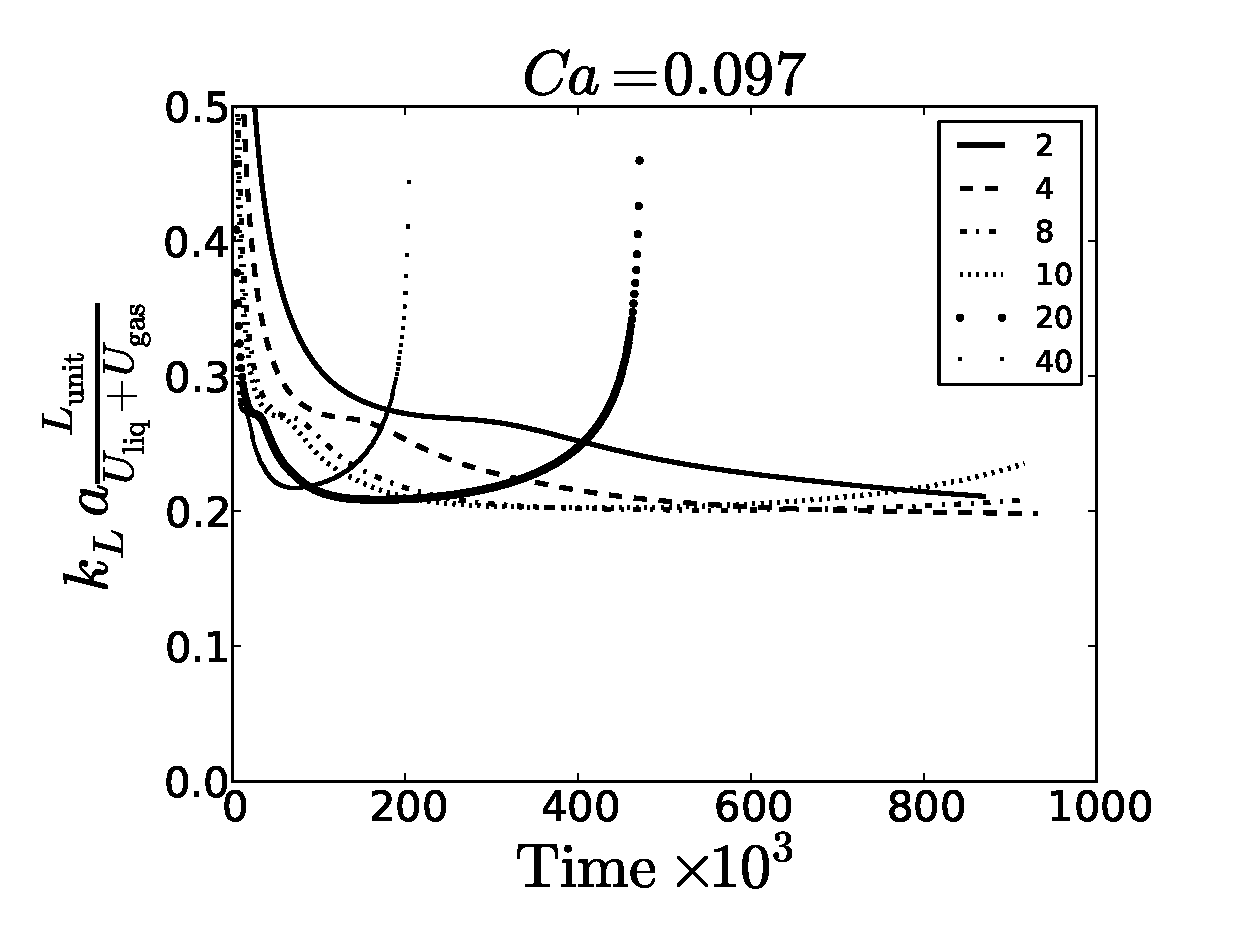
\includegraphics[width=0.5\textwidth]{Figures/aver_conc_scale_ca_time097.eps}
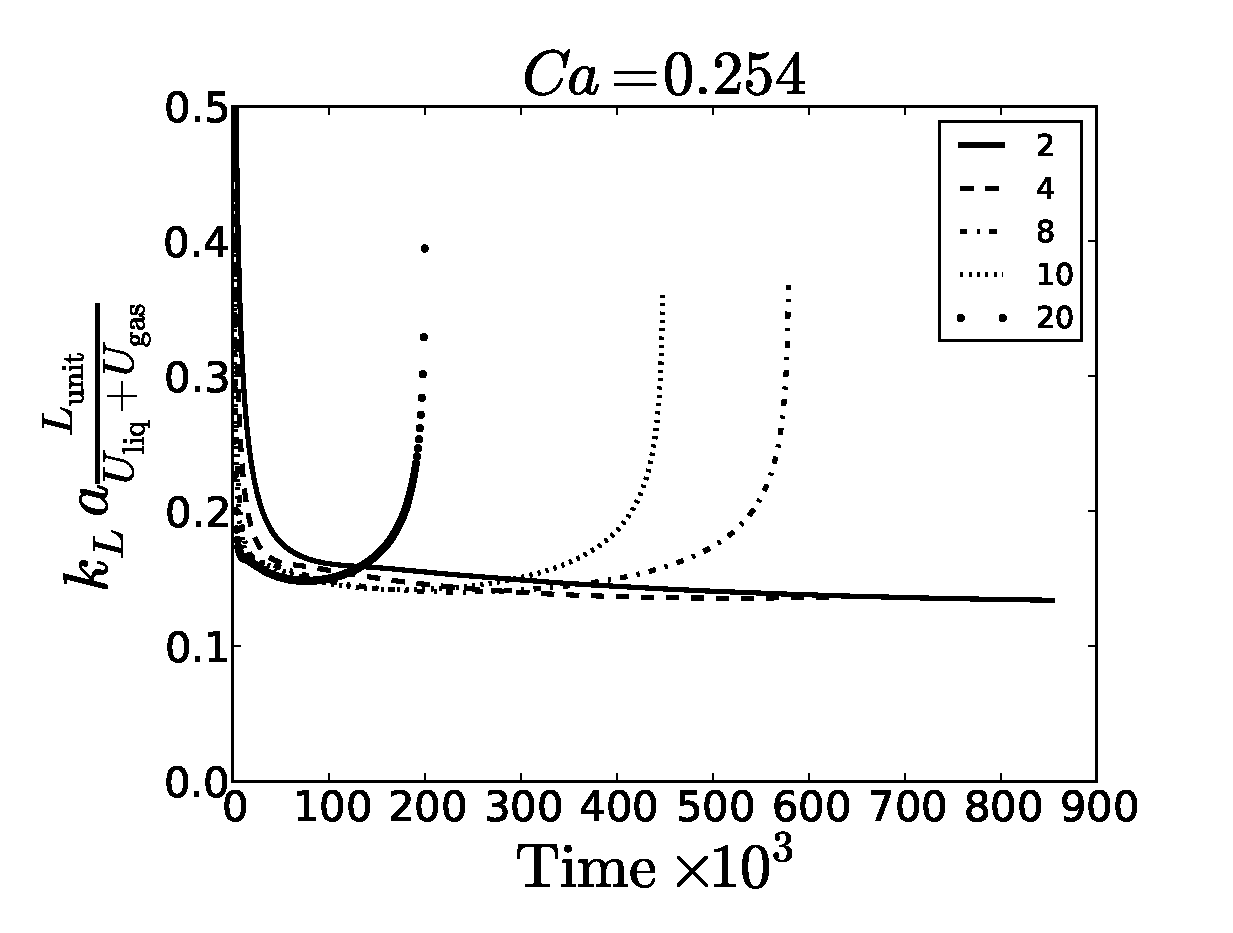
\includegraphics[width=0.5\textwidth]{Figures/aver_conc_scale_ca_time054.eps}\\
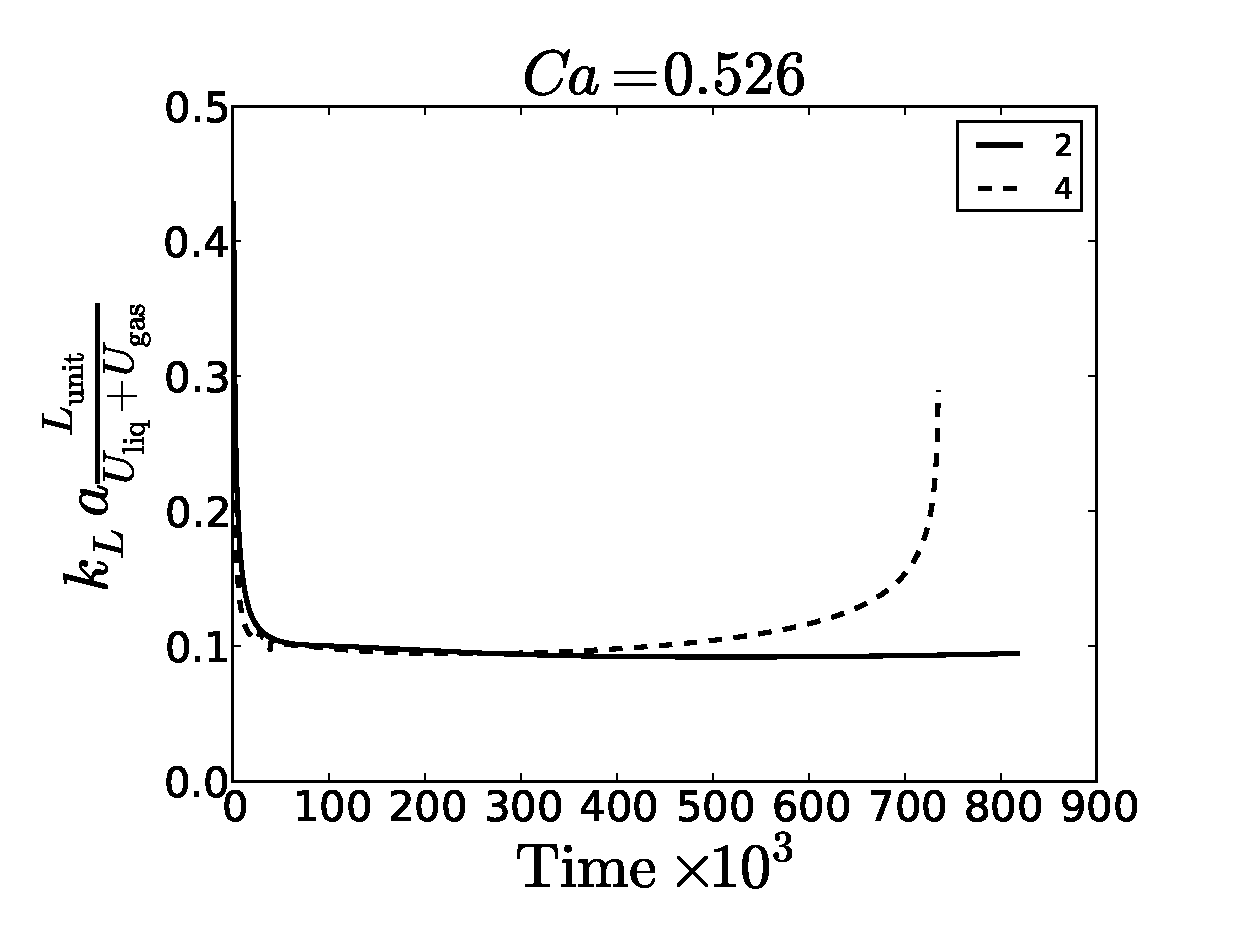
\includegraphics[width=0.5\textwidth]{Figures/aver_conc_scale_ca_time026.eps}
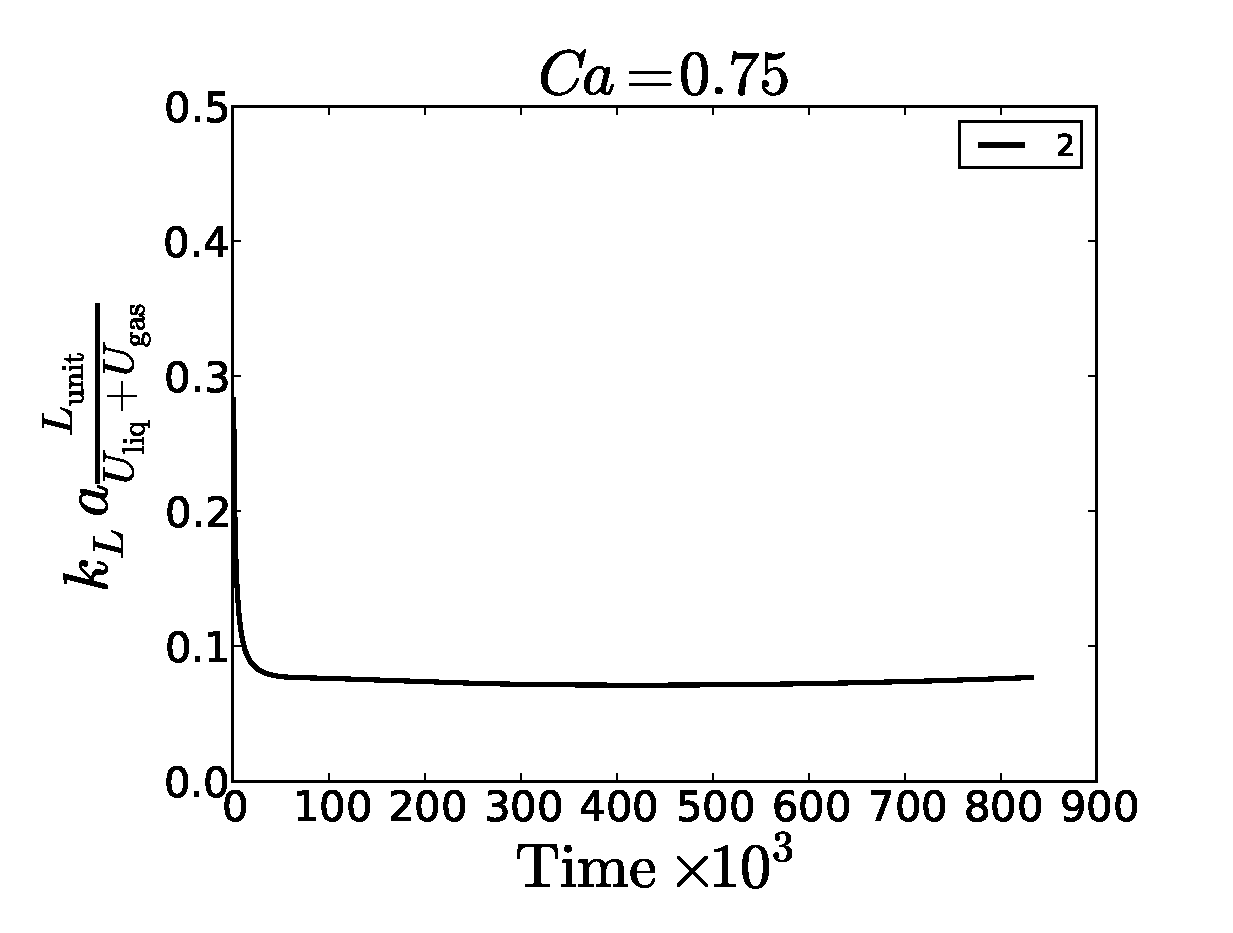
\includegraphics[width=0.5\textwidth]{Figures/aver_conc_scale_ca_time05.eps}\\
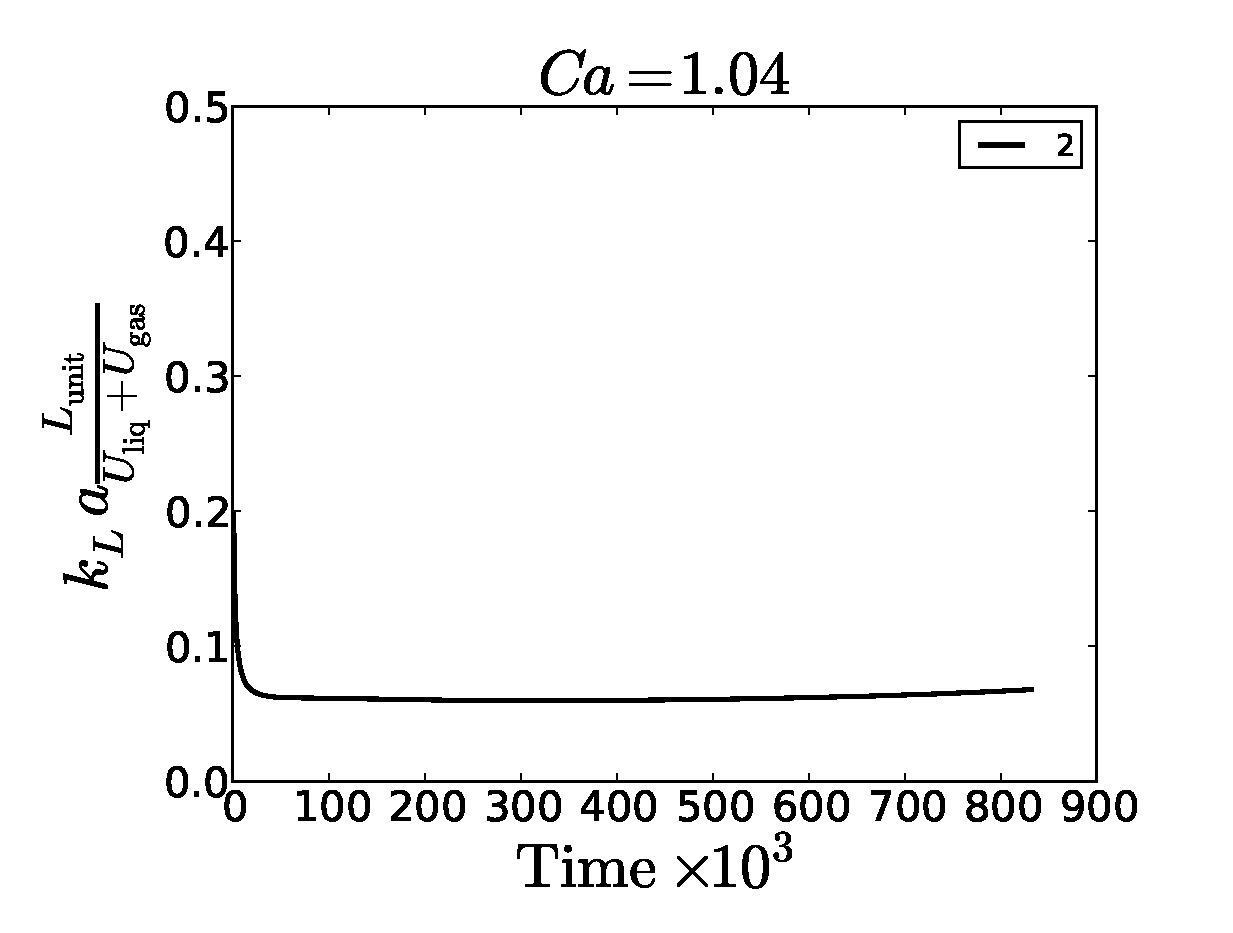
\includegraphics[width=0.5\textwidth]{Figures/aver_conc_scale_ca_time14.eps}
\caption{Calculated volumetric mass transfer coefficient for different capillaries and scales
against time. One can see
that all curves have the same minimum corresponding to the volumetric mass transfer coefficient.
Some simulations show the volumetric mass transfer coefficient going up due to the average
concentration being close to $\cstar$. All of them show excellent agreement. Note, that with the
scaling one can reduce the amount of calculations drastically. However, one needs to be attentive
because with the large velocity scaling average concentration can fastly approach $\cstar$, thus
getting an infinite volumetric mass transfer coefficient.
\label{fig:aver:conc:different:capillaries:time}}
\end{figure}
\begin{figure}[htb!]
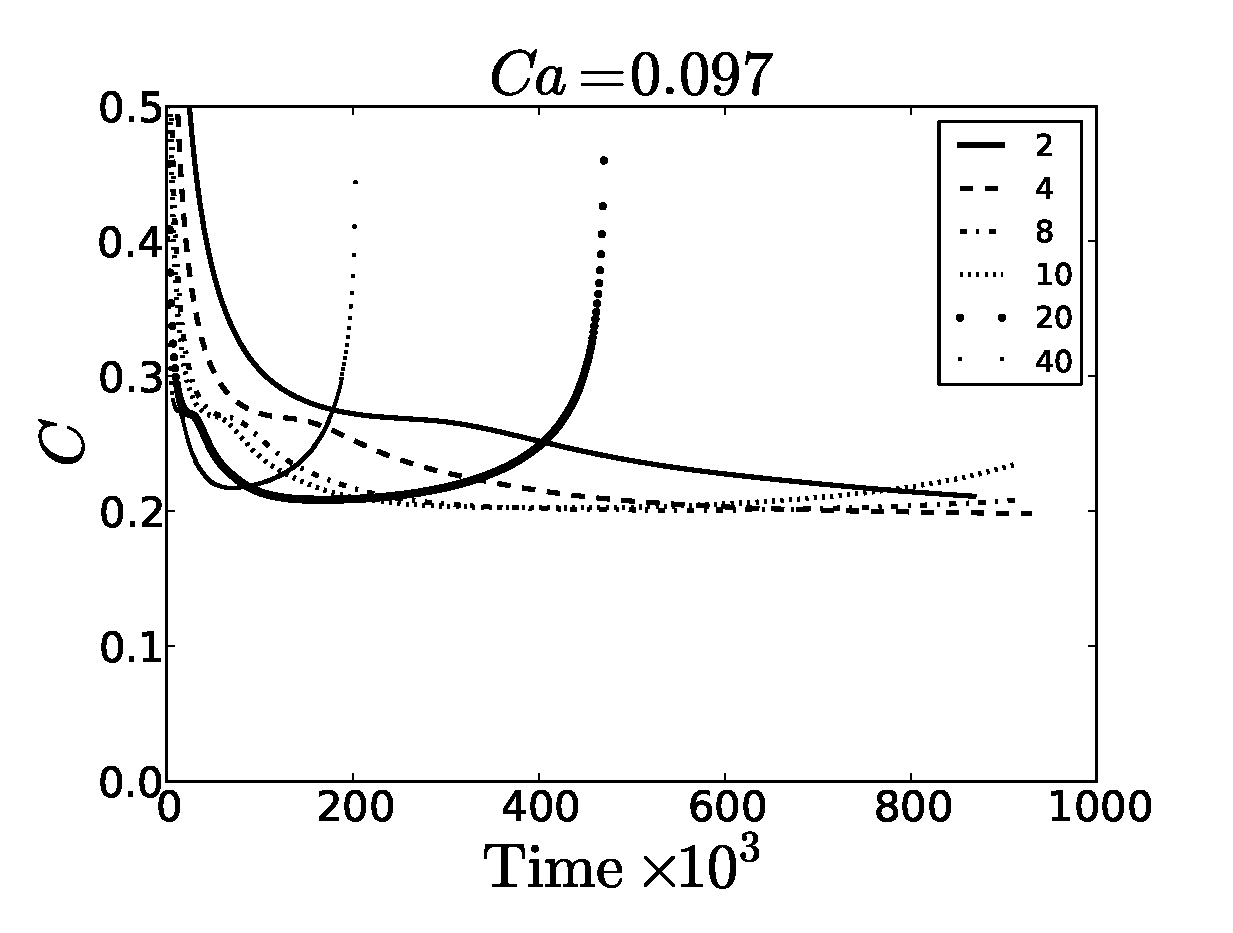
\includegraphics[width=0.5\textwidth]{Figures/aver_conc_scale_ca097.eps}
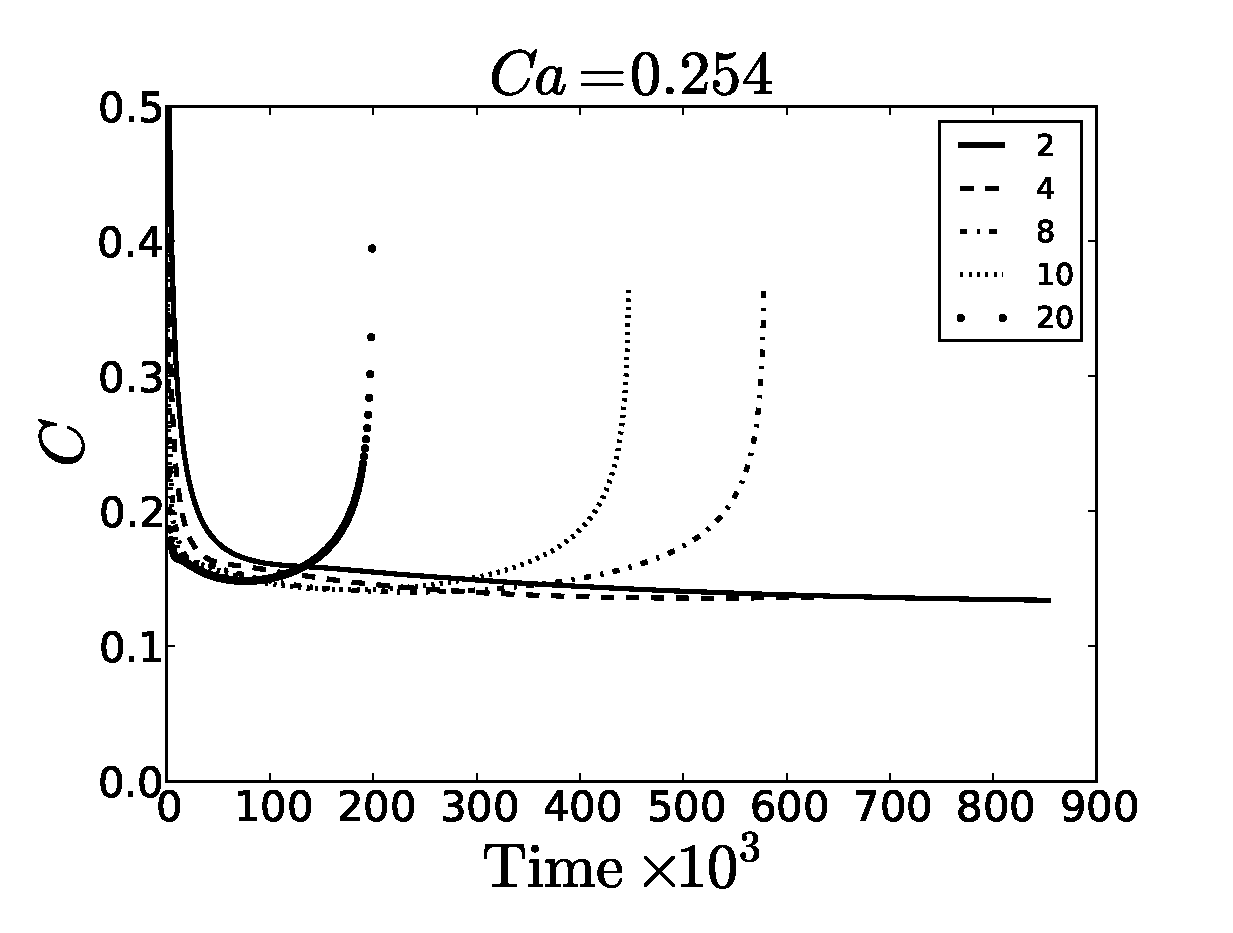
\includegraphics[width=0.5\textwidth]{Figures/aver_conc_scale_ca054.eps}\\
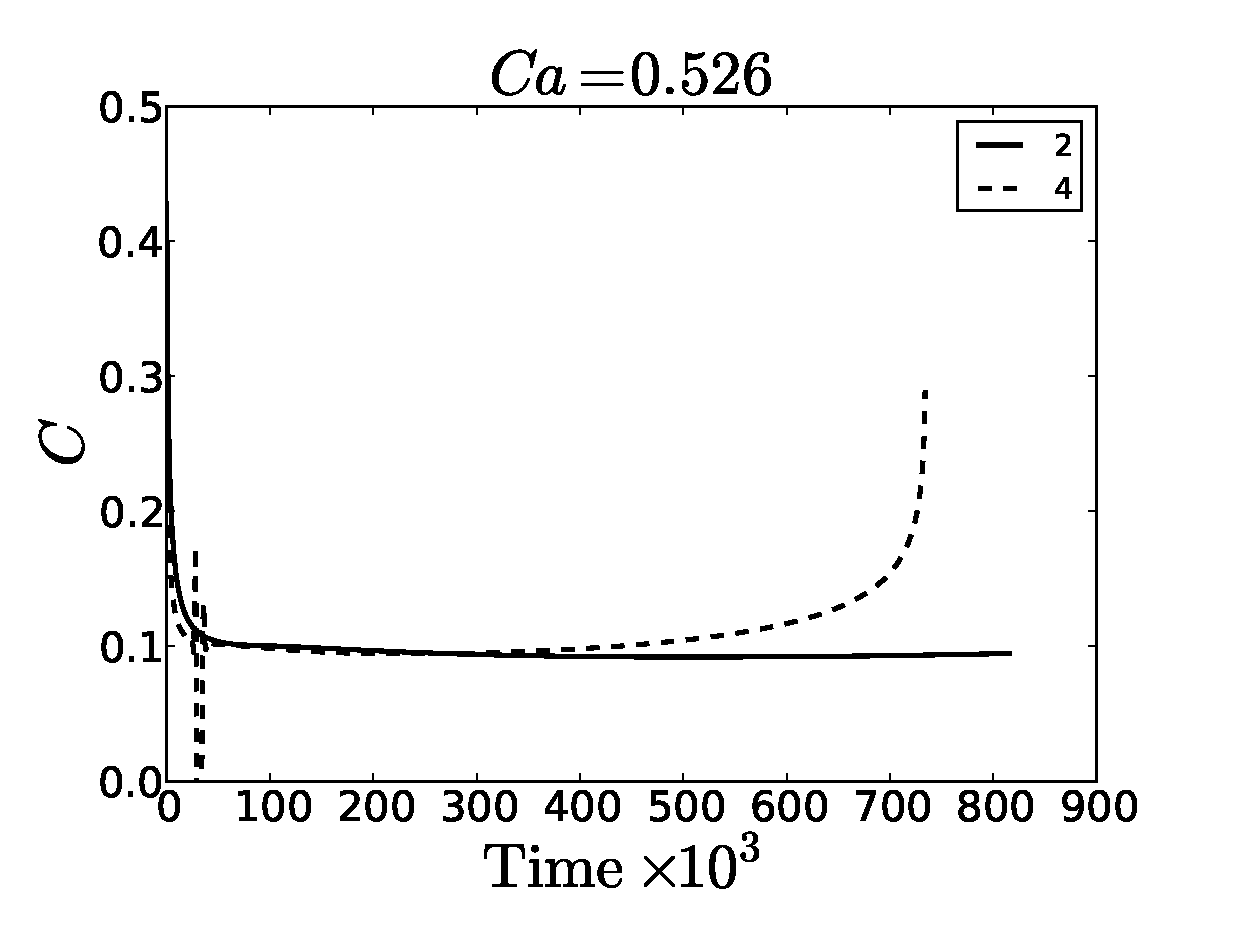
\includegraphics[width=0.5\textwidth]{Figures/aver_conc_scale_ca026.eps}
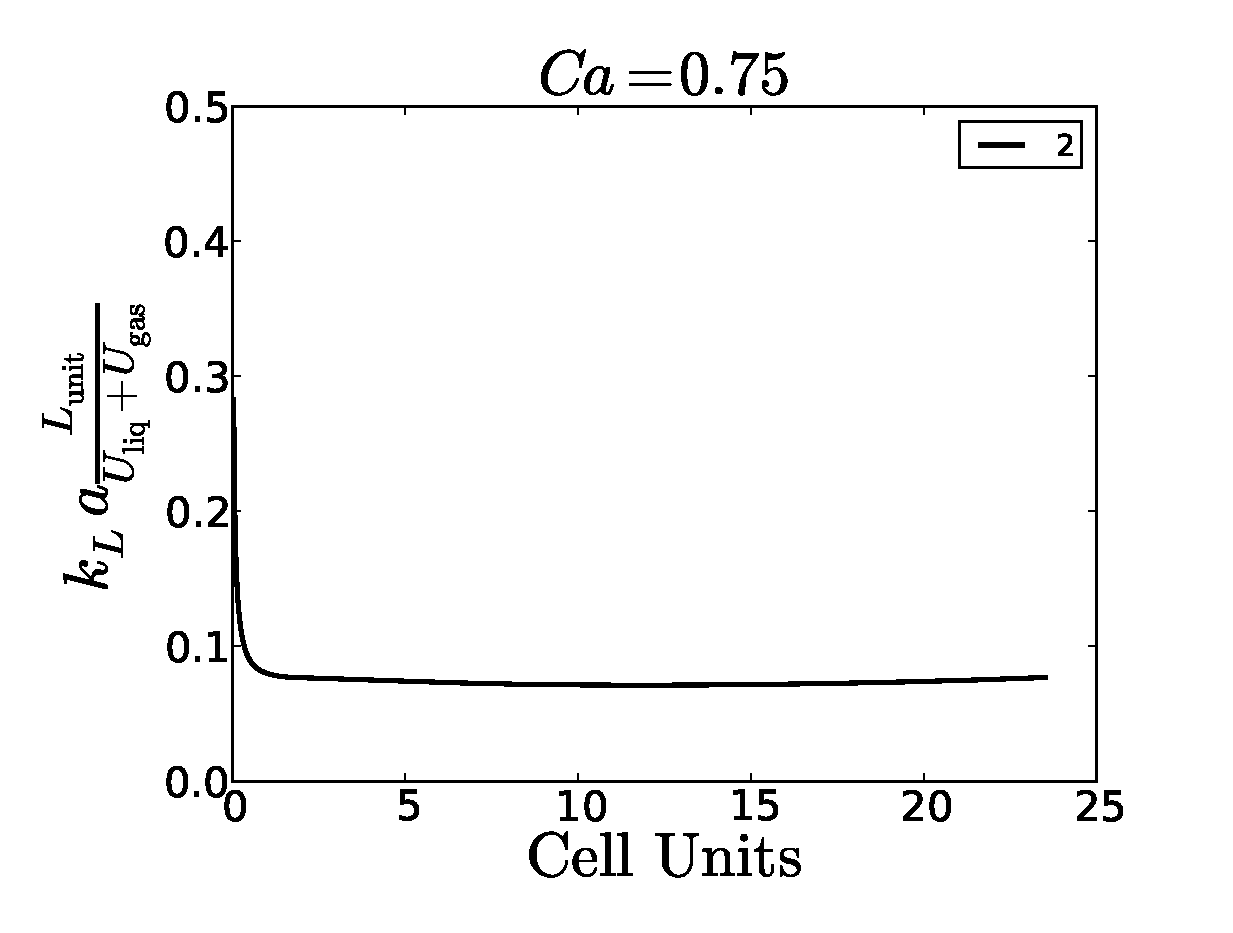
\includegraphics[width=0.5\textwidth]{Figures/aver_conc_scale_ca05.eps}\\
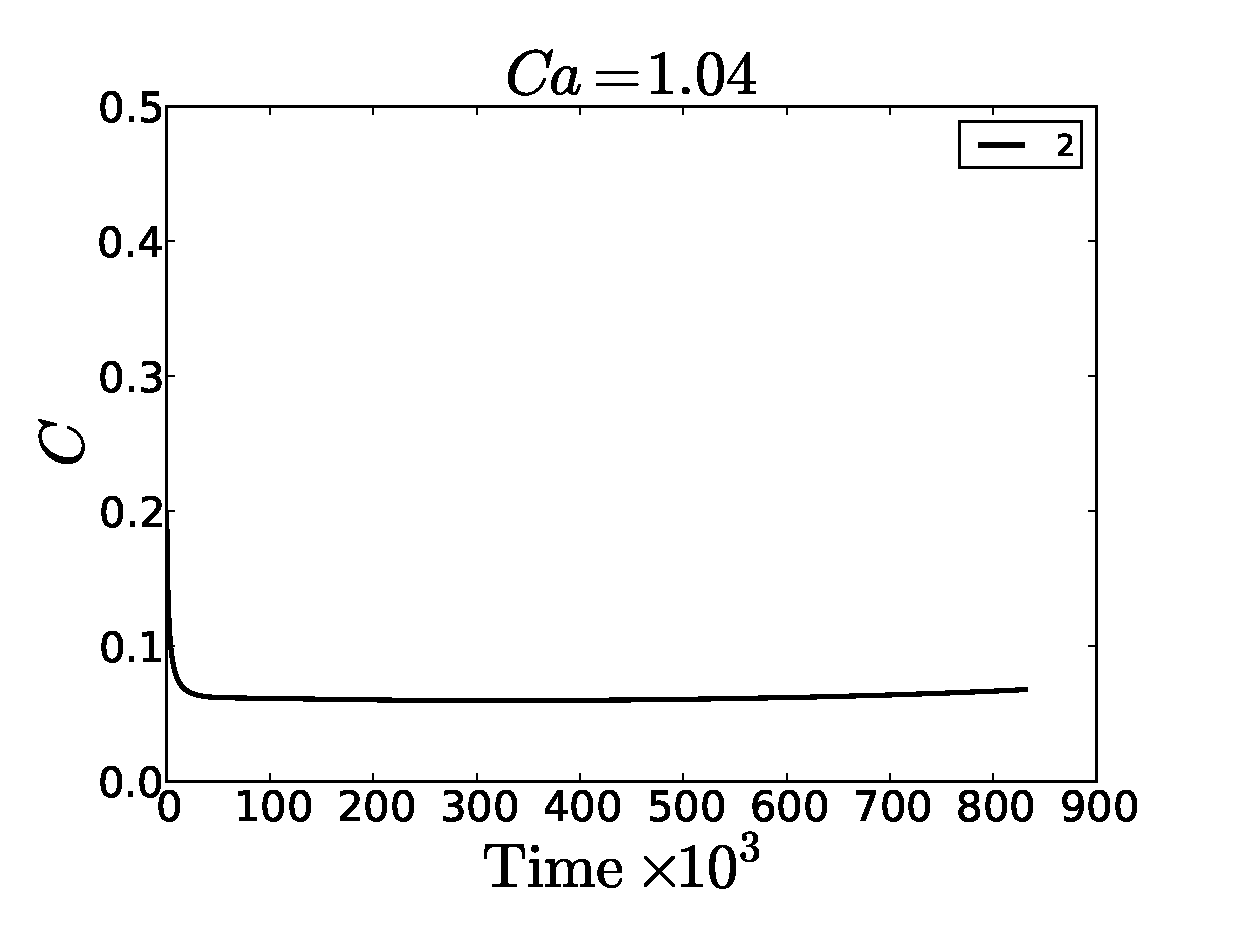
\includegraphics[width=0.5\textwidth]{Figures/aver_conc_scale_ca14.eps}
\caption{Volumetric mass transfer coefficient for different capillaries and scales against the
bubble traveling distance in the laboratory frame. Table \ref{table:steady:state:average}
summarizes results.\label{fig:aver:conc:different:capillaries}}
\end{figure}
\begin{table}[htb!]
\begin{tabularx}{\textwidth}{|X|X|X|X|}
\hline
$Ca$    &$Pe$     &$L_{\mathrm{steady}}/\lunit$& $\volnondim$ \\
\hline
$0.097$ &$1313$  &$7$&$0.21$  \\ 
$0.254$ &$3414$  &$6$&$0.14$  \\ 
$0.526$ &$7092$  &$3$&$0.095$ \\
$0.750$ &$10125$ &$3$&$0.074$ \\
$1.040$ &$14041$ &$2$&$0.0601$\\
\hline
\end{tabularx}
\caption{The distance which a bubble propagates when the
steady-state condition is achieved. One can see that increasing
Peclet number helps to achieve the steady state faster.\label{table:steady:state:average}}
\end{table}

\subsection{Periodic boundaries with the inlet/outlet characteristic concentration}
When the characteristic concentration is taken as in the formulation of \citet{vanbaten-circular},
i.e. the inlet/outlet flux averaged concentration, then the results are quite different. One can
see in Fig. \ref{fig:volumetric:char:concentration:vanbaten} the calculated volumetric mass transfer
is different from the domain averaged calculated volumetric mass transfer coefficient. For example,
for small capillary numbers, i.e. $Ca=0.097,0.254,0.526$ the predicted values are overpredicted
($\volnondim=0.3,0.25,0.1$). When the pattern is changed, i.e. $Ca=0.75,1.04$ the calculated values
are underpredicted than in previous case, i.e. $\volnondim=0.06,0.04$.
\begin{figure}[htb!]
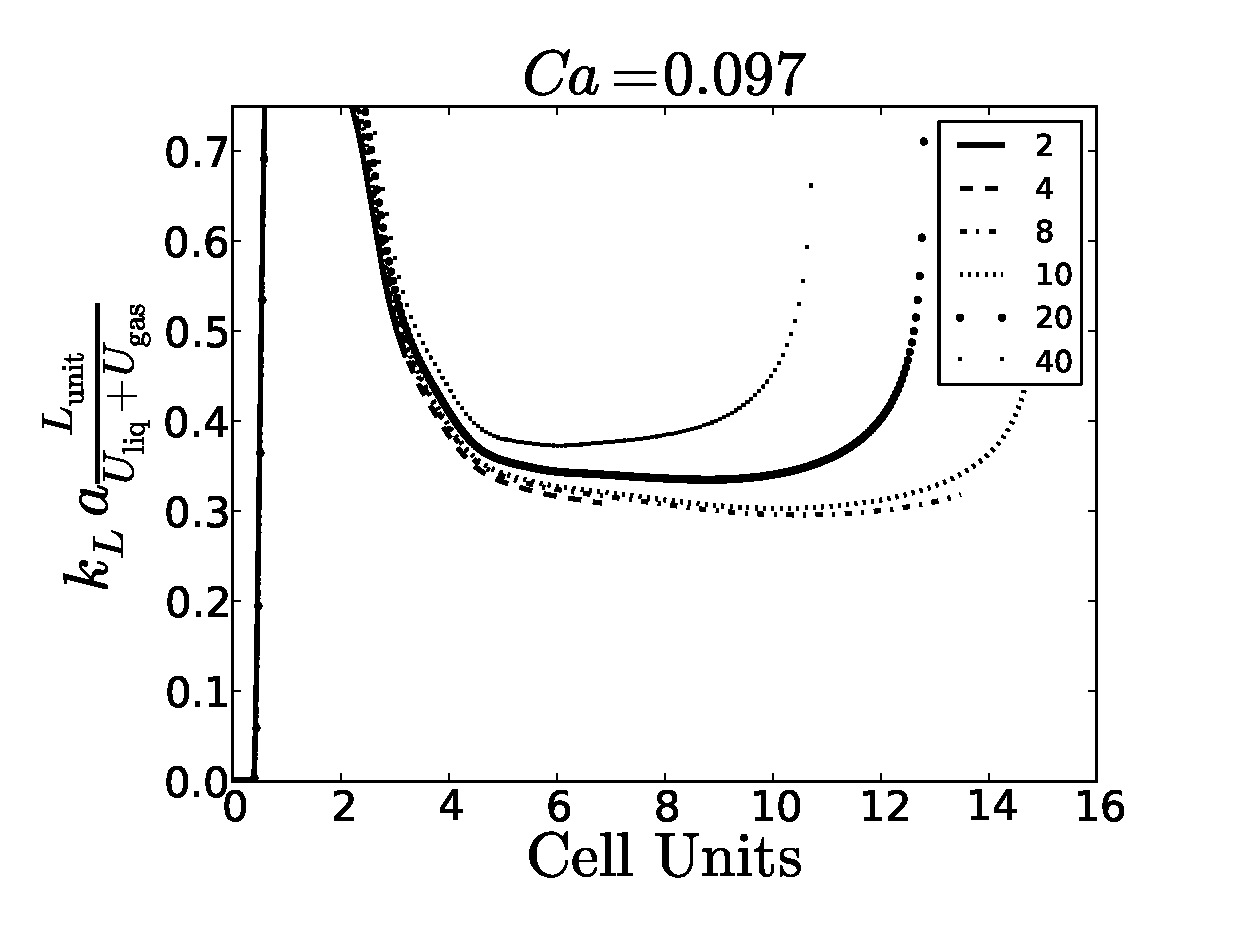
\includegraphics[width=0.5\textwidth]{Figures/aver_vanbaten_scale_ca097.eps}
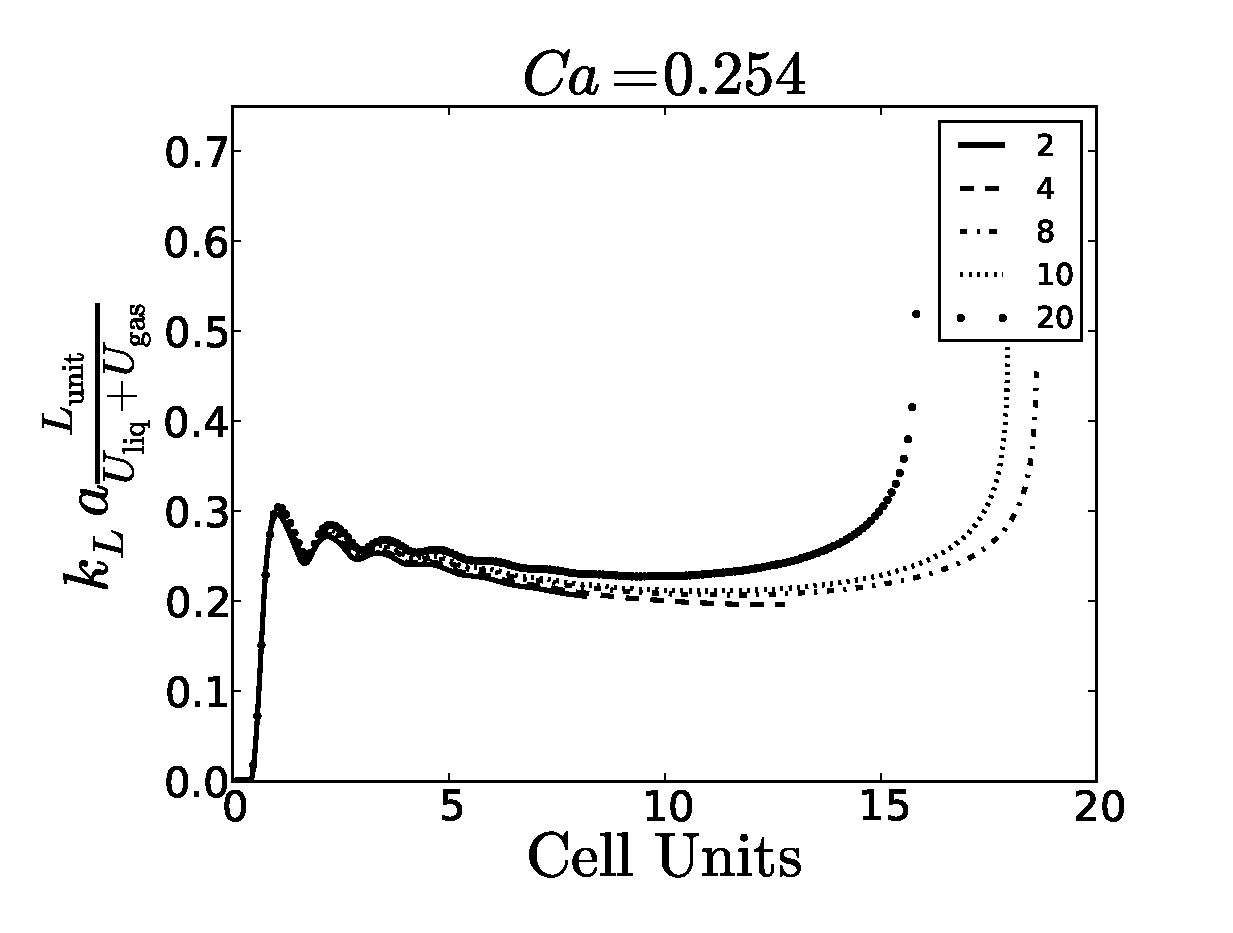
\includegraphics[width=0.5\textwidth]{Figures/aver_vanbaten_scale_ca054.eps}\\
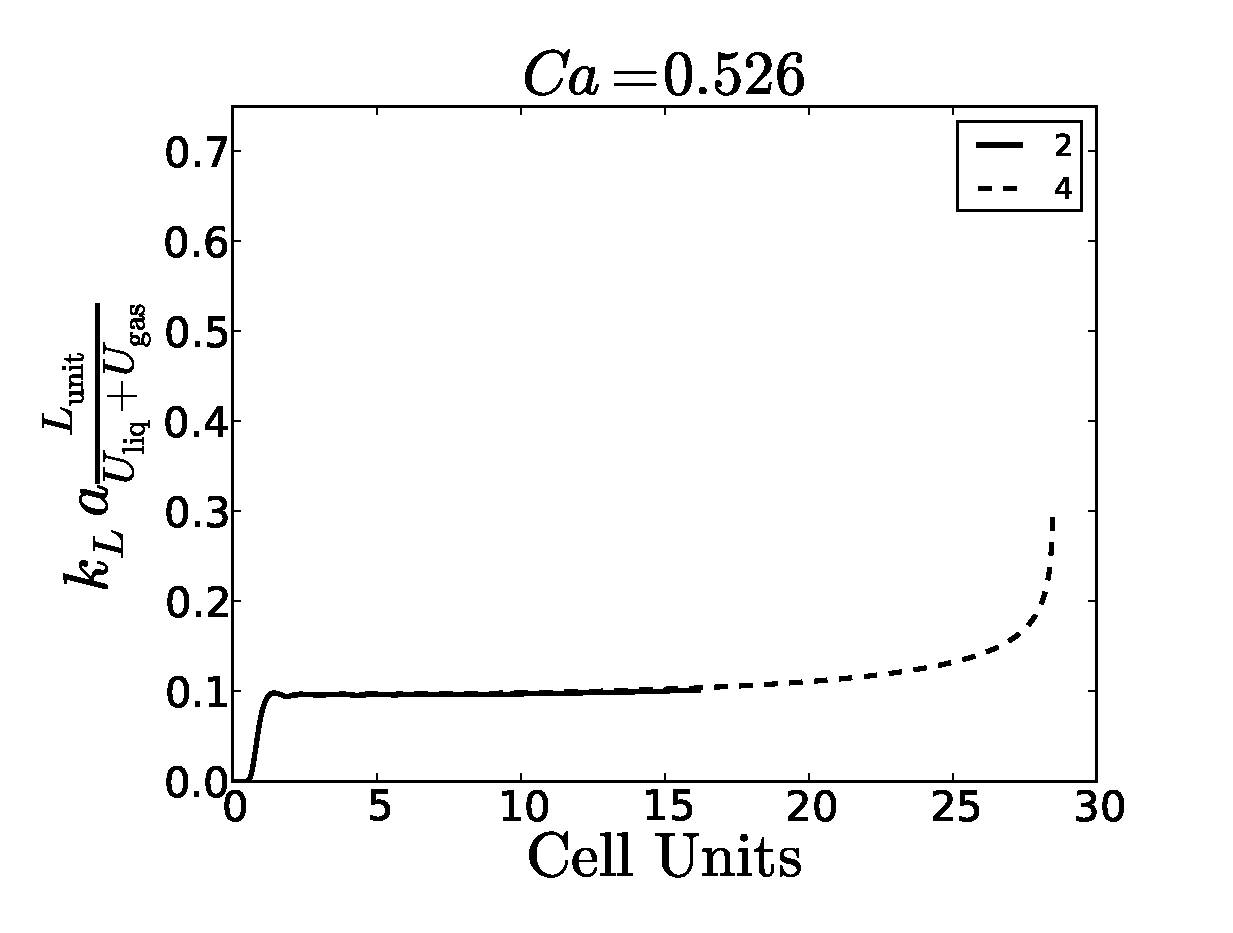
\includegraphics[width=0.5\textwidth]{Figures/aver_vanbaten_scale_ca026.eps}
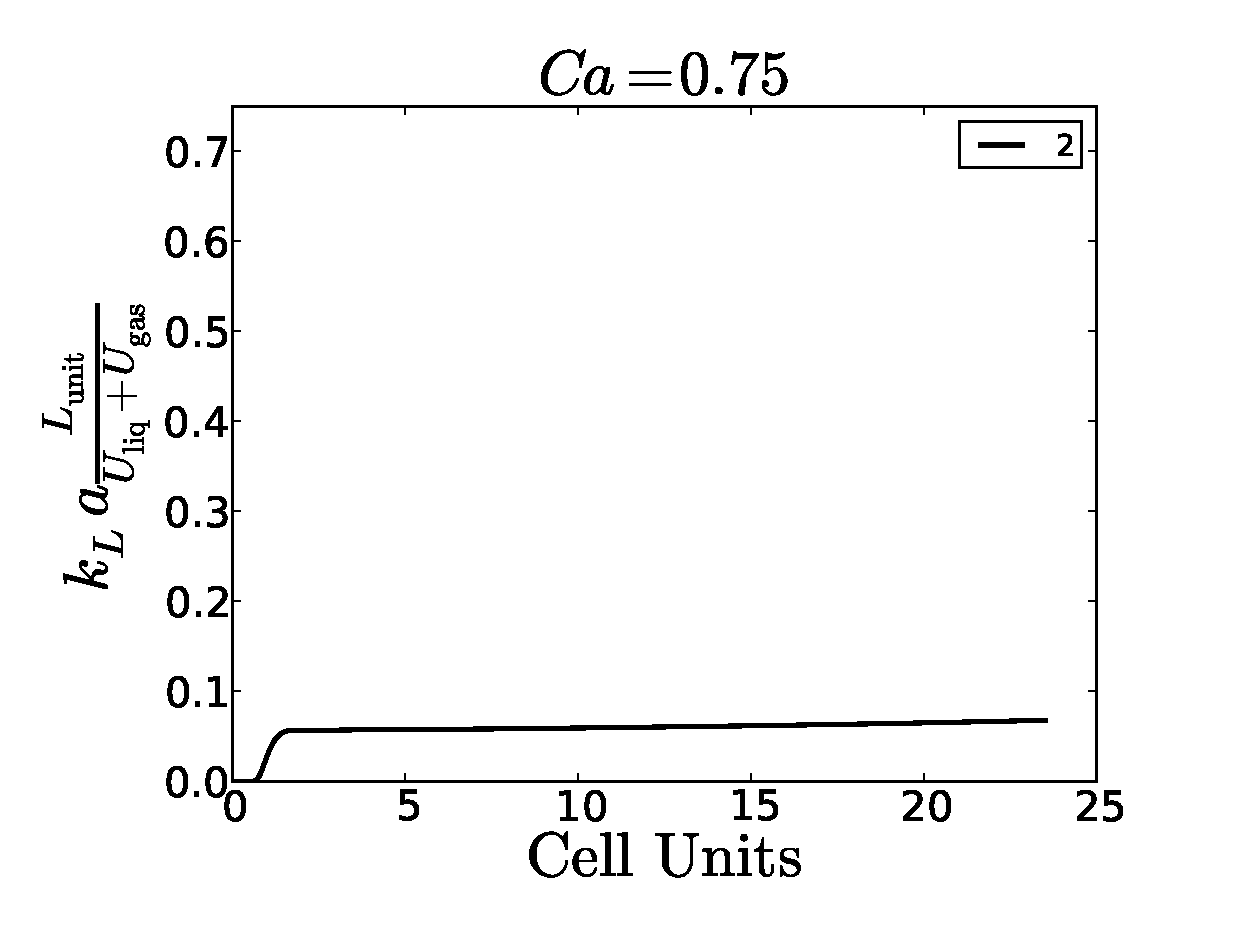
\includegraphics[width=0.5\textwidth]{Figures/aver_vanbaten_scale_ca05.eps}\\
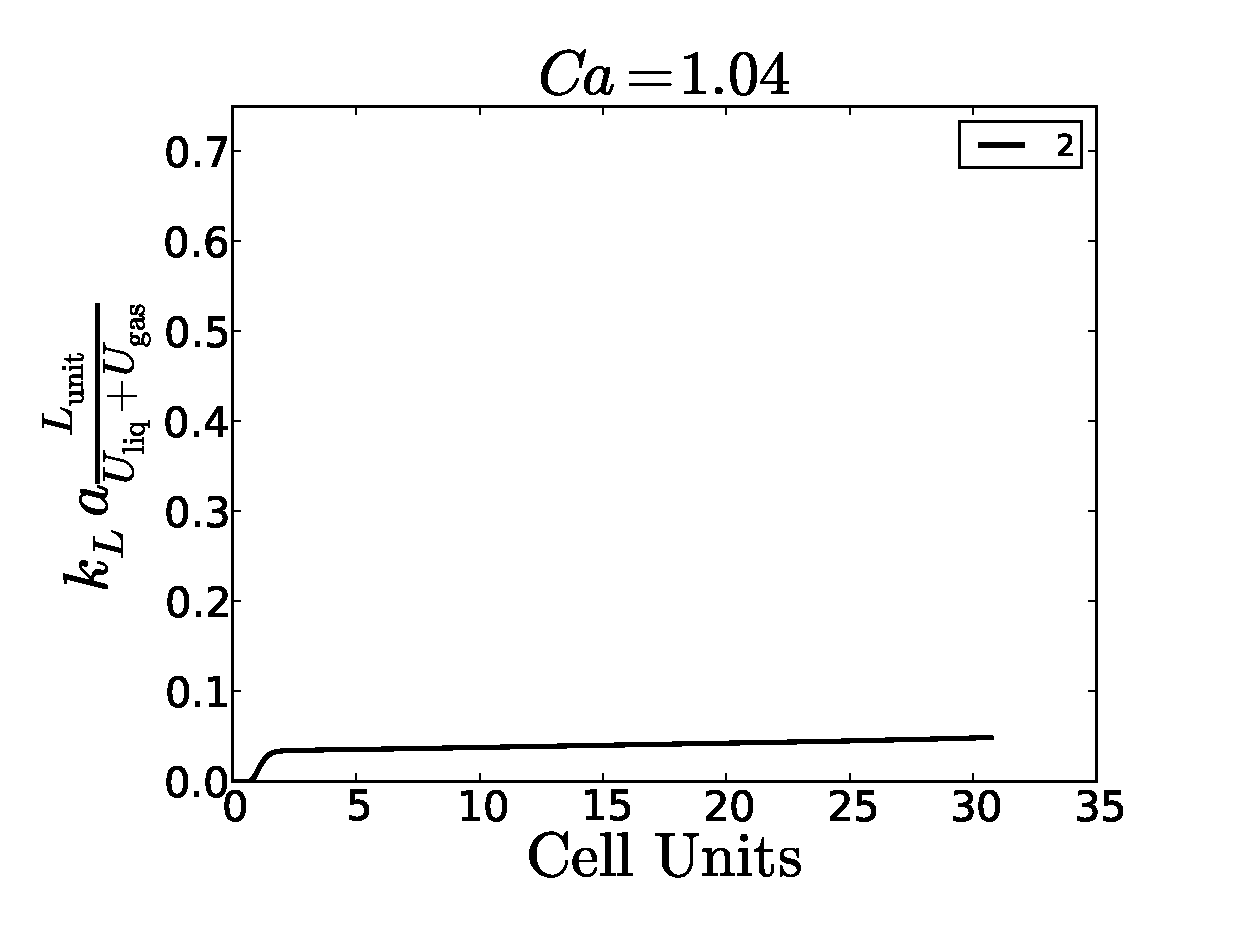
\includegraphics[width=0.5\textwidth]{Figures/aver_vanbaten_scale_ca14.eps}
\caption{The volumetric mass transfer coefficient
with the characteristic concentration based on
the inlet/outlet flux averaged concentration as
in \cite{vanbaten-circular}. One can see that values are either overpredicted or underpredicted
than values specified in Table \ref{table:steady:state:average} depending on the velocity pattern. 
\label{fig:volumetric:char:concentration:vanbaten}}
\end{figure}



\subsection{\citeauthor{vanbaten-circular} formulation}
The van Baten formulation which is calculated as the change of mass in domain with characteristic
concentrations to be as the average domain simulation and as the averaged flux input/output
concentration. One can see them in Fig. \ref{fig:vanbaten} for $Ca=0.097$ and
$Ca=1.04$. One can see that results are consistent with the simulations in Section
\ref{main:results:periodic} for the volumetric mass transfer coefficient measured with the domain
averaged concentration in the whole range of capillary numbers. Note that for $Ca=0.097$ the
obtained mass transfer coefficient is less than in Section \ref{main:results:periodic}. However, as
it will be shown later this coefficient coincides with the many units formulation. The inlet/outlet
flux averaged concentration is shown to be consistent only for velocity patterns related to larger
Capillary numbers, i.e. $Ca\geq0.7$. 
\begin{figure}
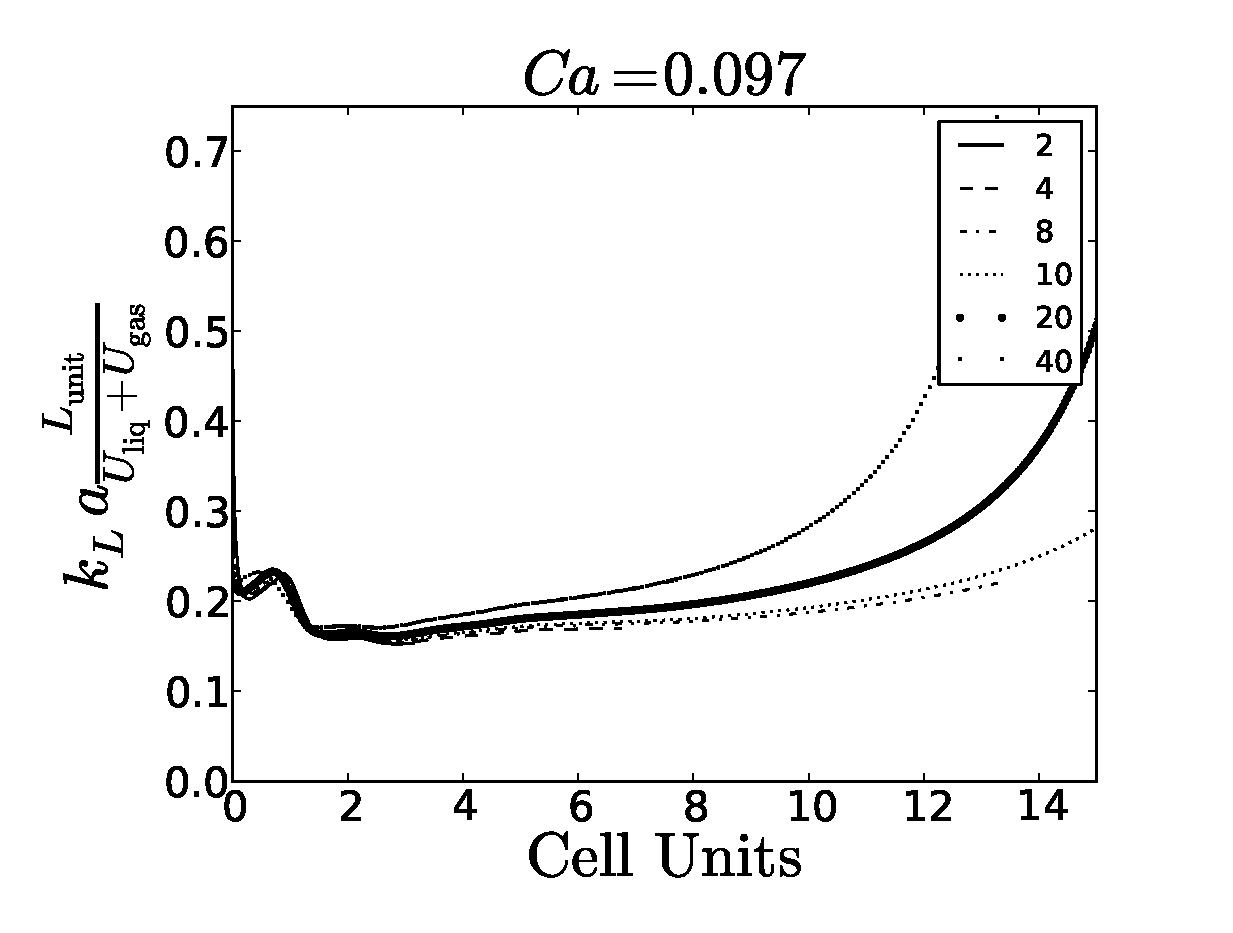
\includegraphics[width=0.5\textwidth]{Figures/vanbaten_aver_scale_ca097.eps}
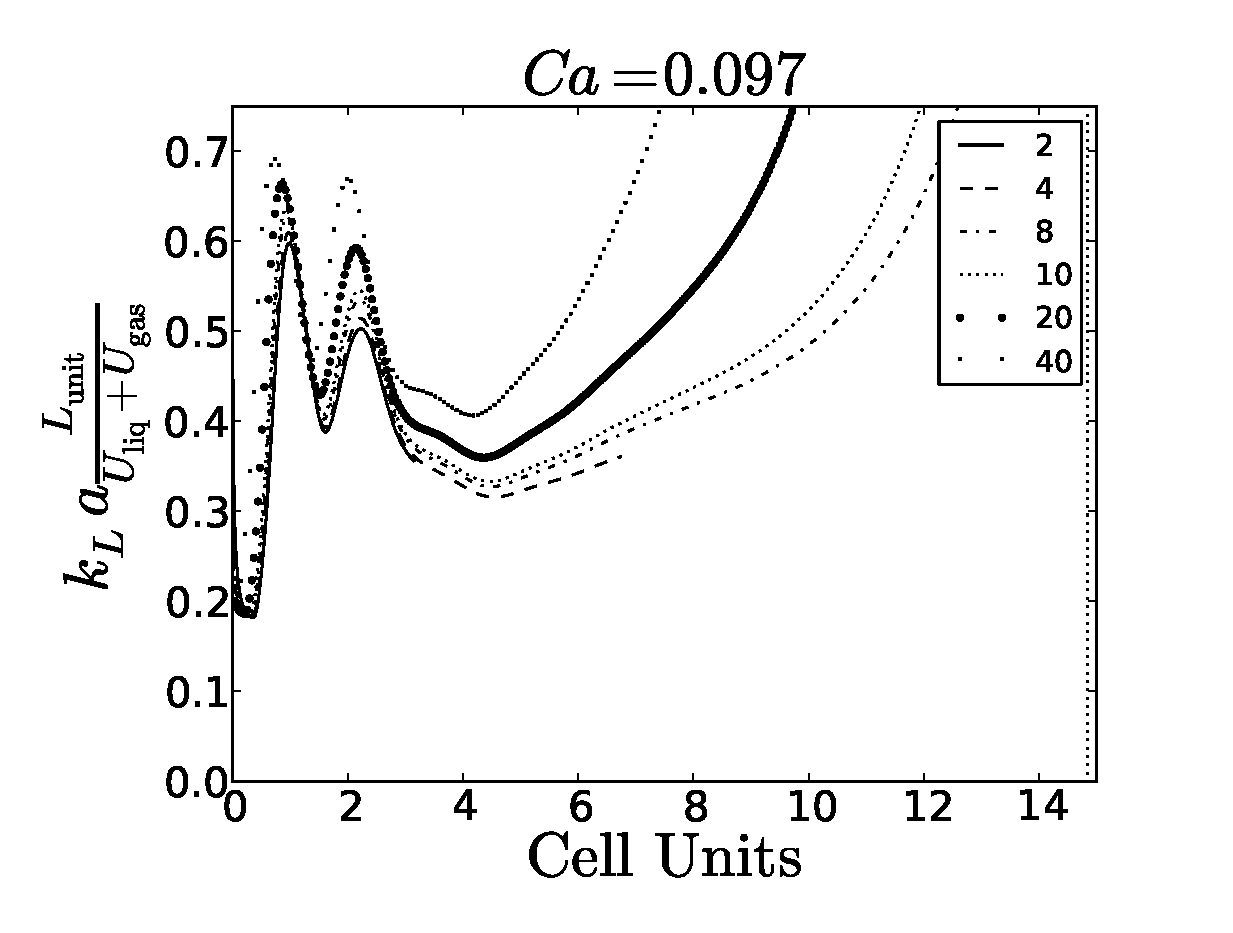
\includegraphics[width=0.5\textwidth]{Figures/vanbaten_full_scale_ca097.eps}\\
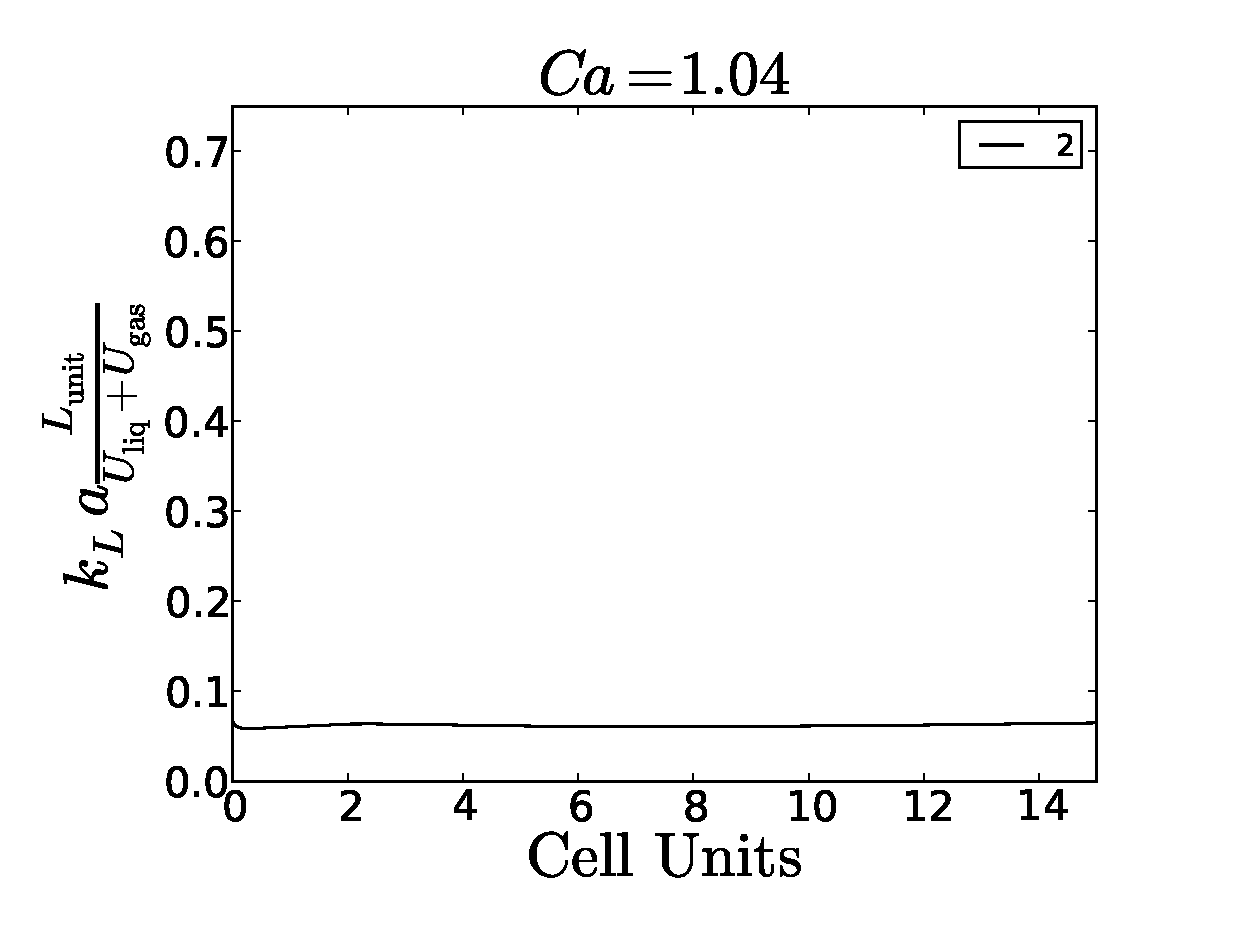
\includegraphics[width=0.5\textwidth]{Figures/vanbaten_aver_scale_ca14.eps}
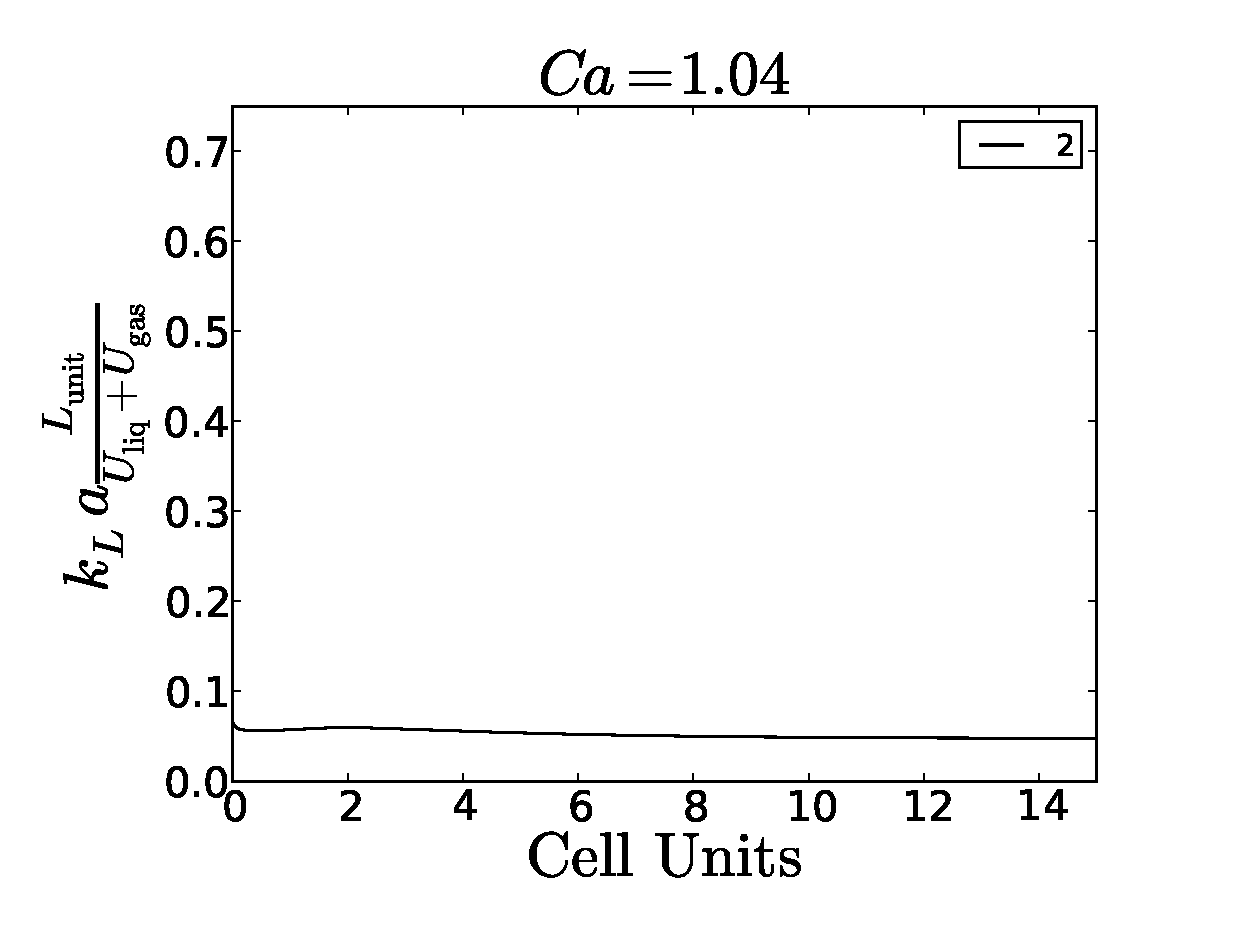
\includegraphics[width=0.5\textwidth]{Figures/vanbaten_full_scale_ca14.eps}\\
\caption{The \citet{vanbaten-circular} formulations for $Ca=0.097$ (top) and
$Ca=1.04$ (bottom) with the characteristic concentration being domain
averaged (left) and inlet/outlet flux averaged concentration (right). One can
see that \citet{vanbaten-circular} formulation is good with the average
characteristic concentration for capillary numbers regimes without
vortex. Moreover, the values are more close to values obtained with many cells
simulations, see Fig. \ref{fig:moving:average:ca0097}. However, the characteristic concentration
being inlet/outlet flux averaged concentration does not produce consistent results.
\label{fig:vanbaten}}
\end{figure}

%\section{Open boundary conditions}
%\begin{figure}
%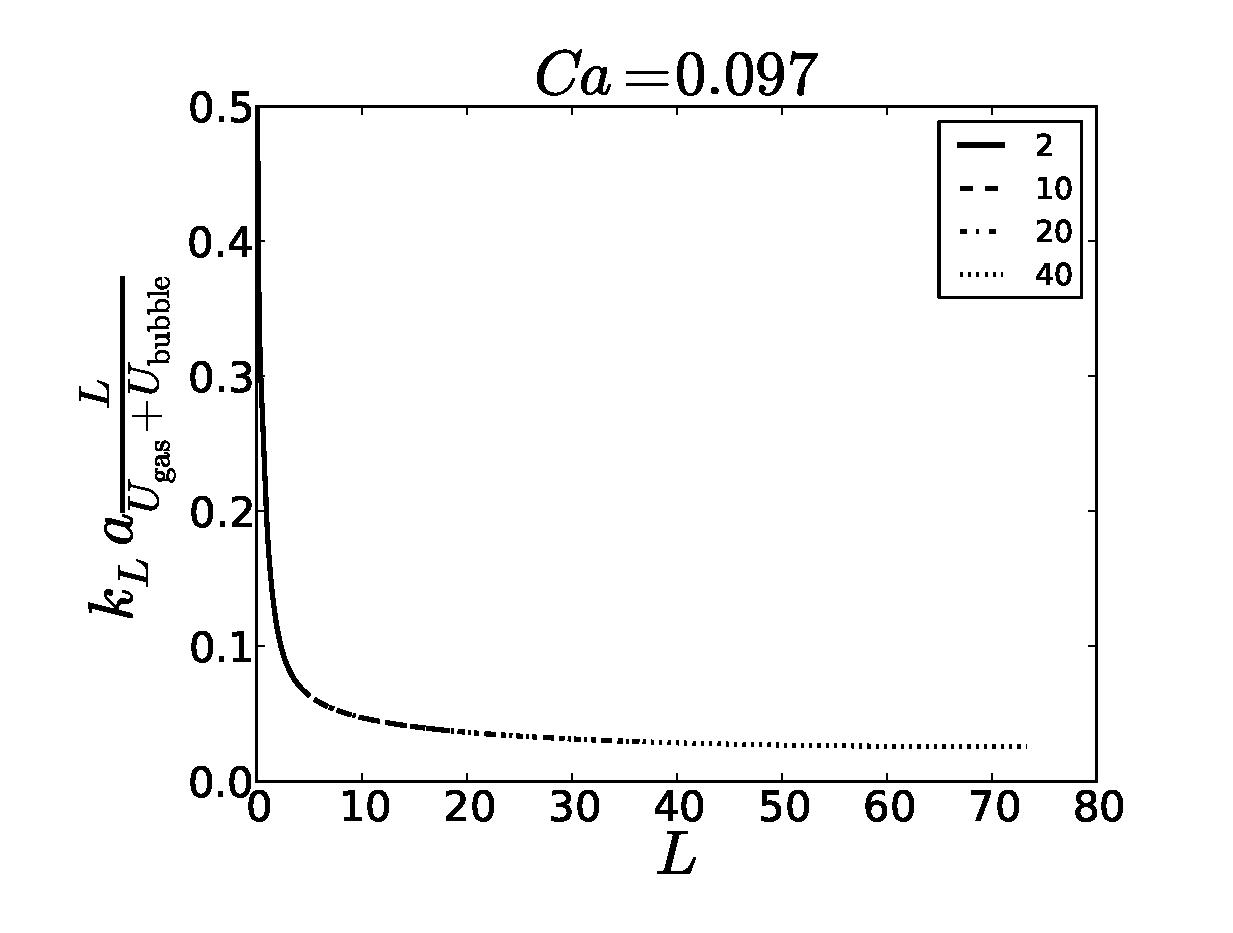
\includegraphics[width=0.5\textwidth]{Figures/jos_aver_conc_scale_ca0097.eps}
%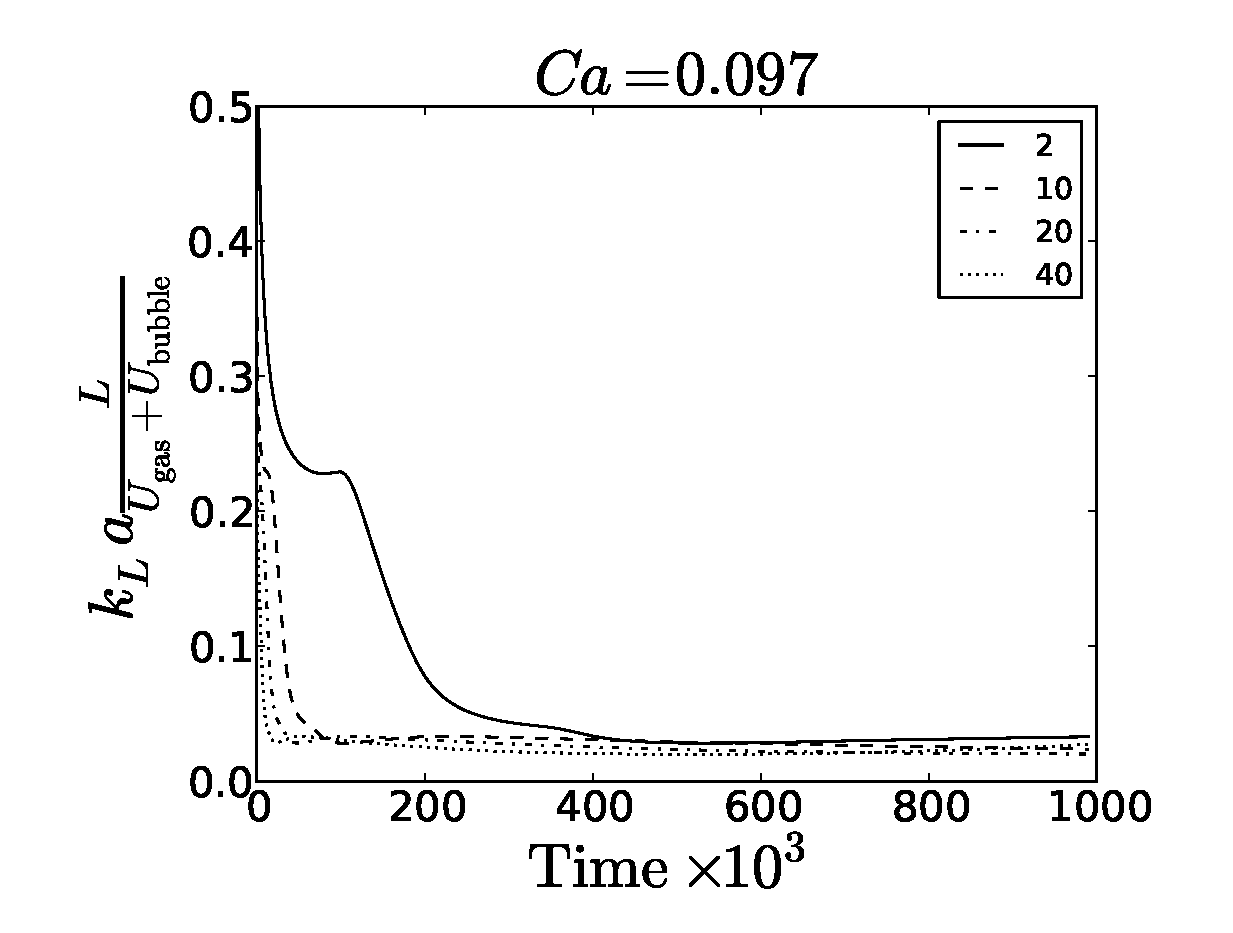
\includegraphics[width=0.5\textwidth]{Figures/jos_aver_moving_window_ca0097.eps}\\
%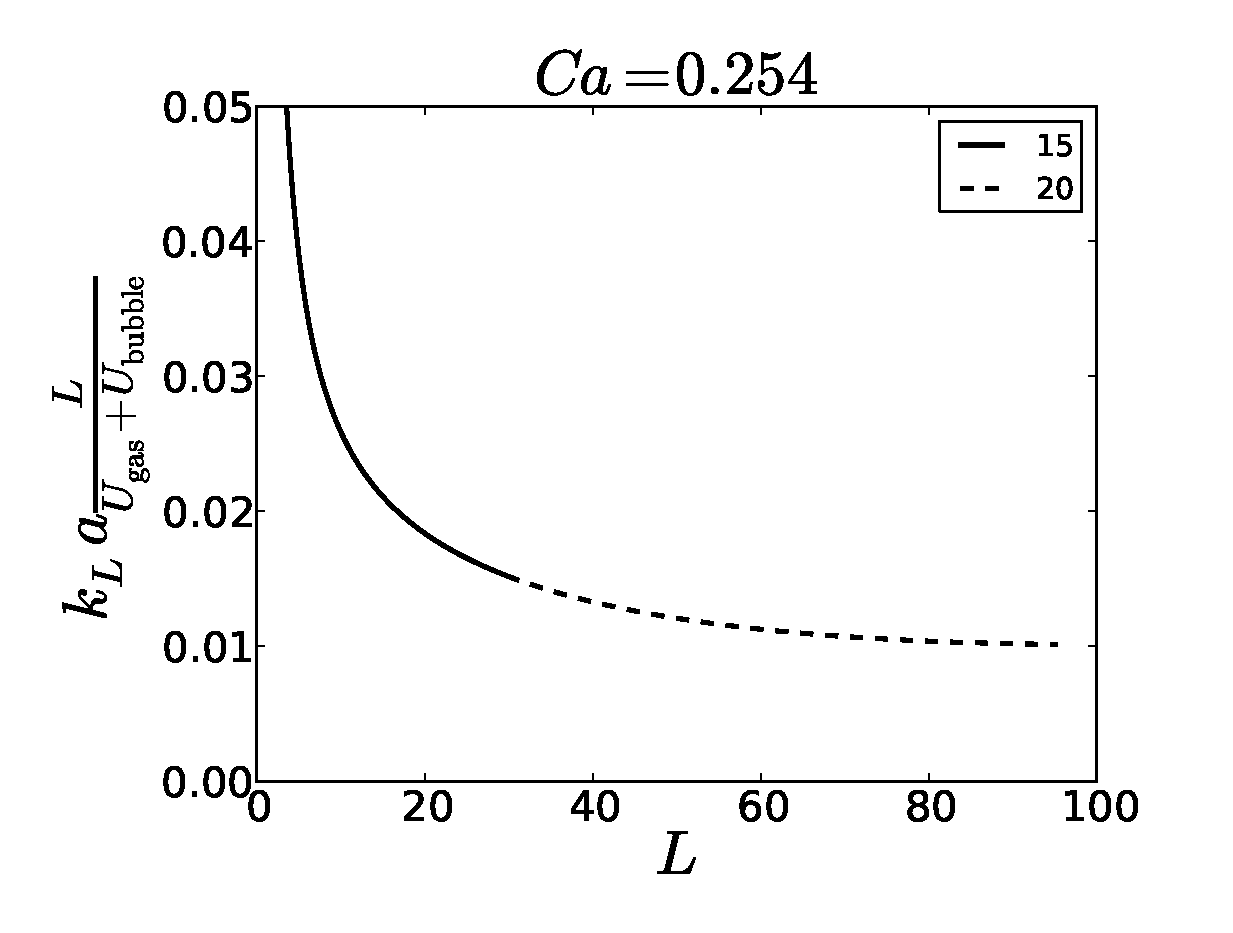
\includegraphics[width=0.5\textwidth]{Figures/jos_aver_conc_scale_ca0254.eps}
%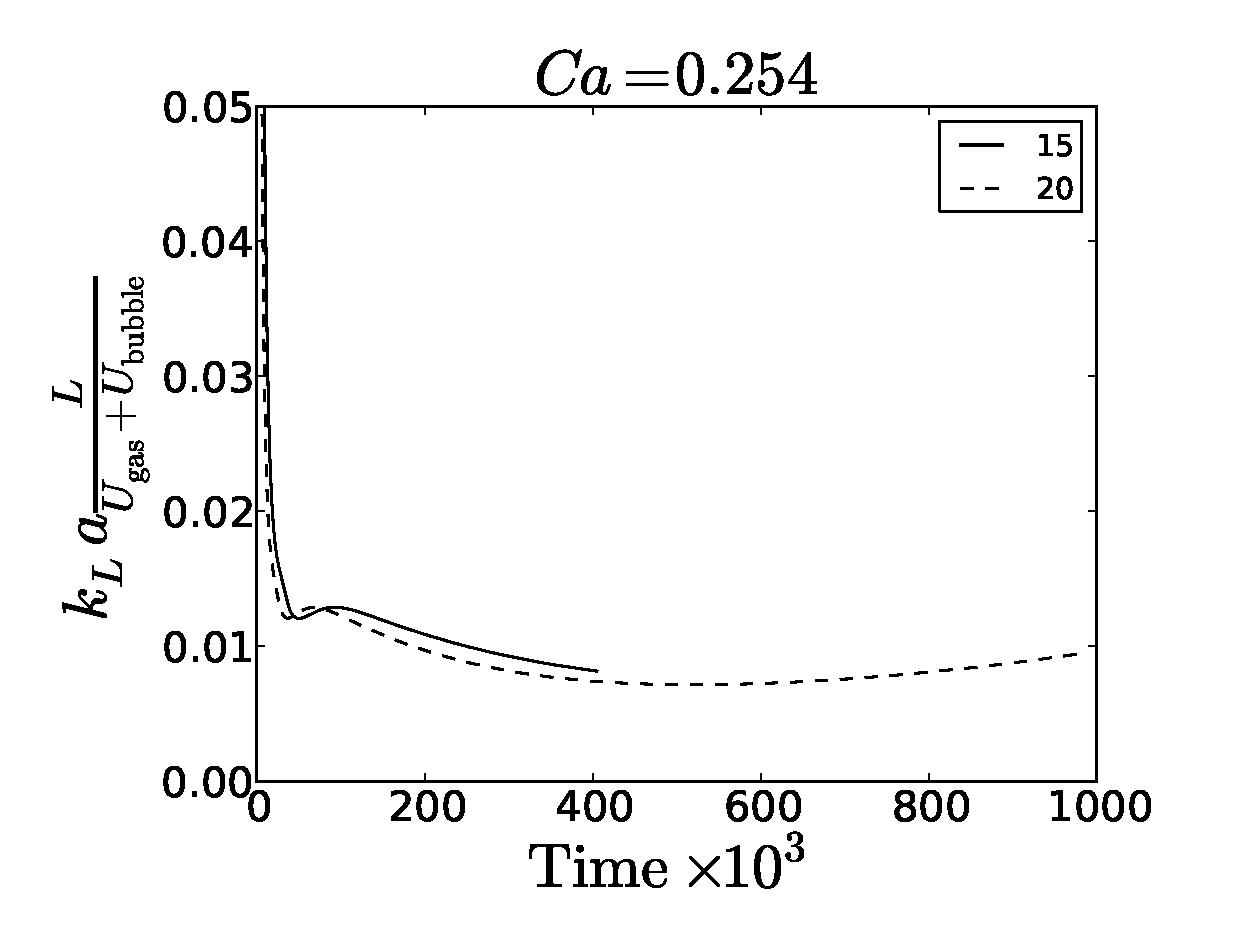
\includegraphics[width=0.5\textwidth]{Figures/jos_aver_moving_window_ca0254.eps}\\
%\caption{Open boundary conditions. \label{fig:open:boundary:jos}}
%\end{figure}
%\section{Symmetric boundary conditions}
%\begin{figure}
%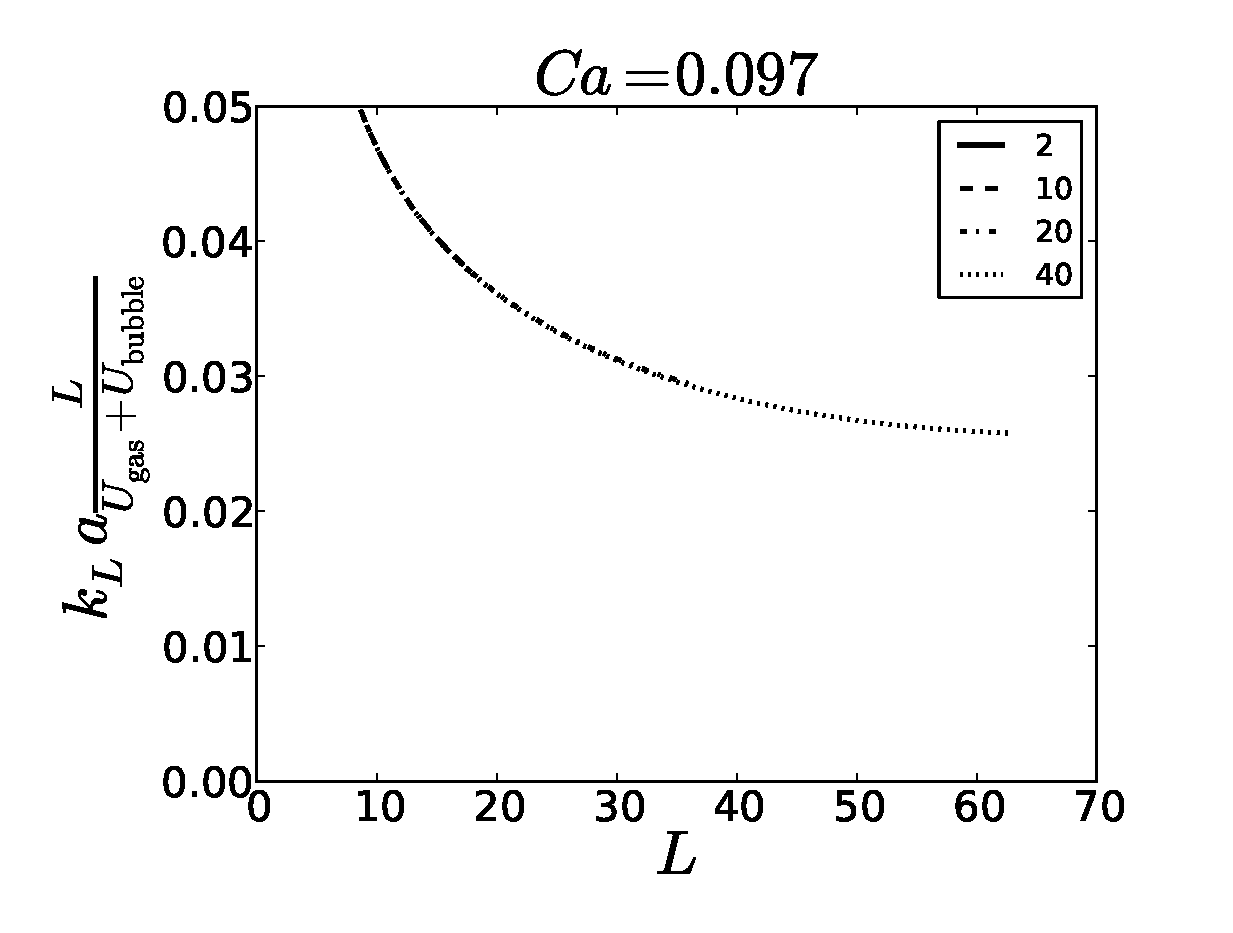
\includegraphics[width=0.5\textwidth]{Figures/sym_aver_conc_scale_ca0097.eps}
%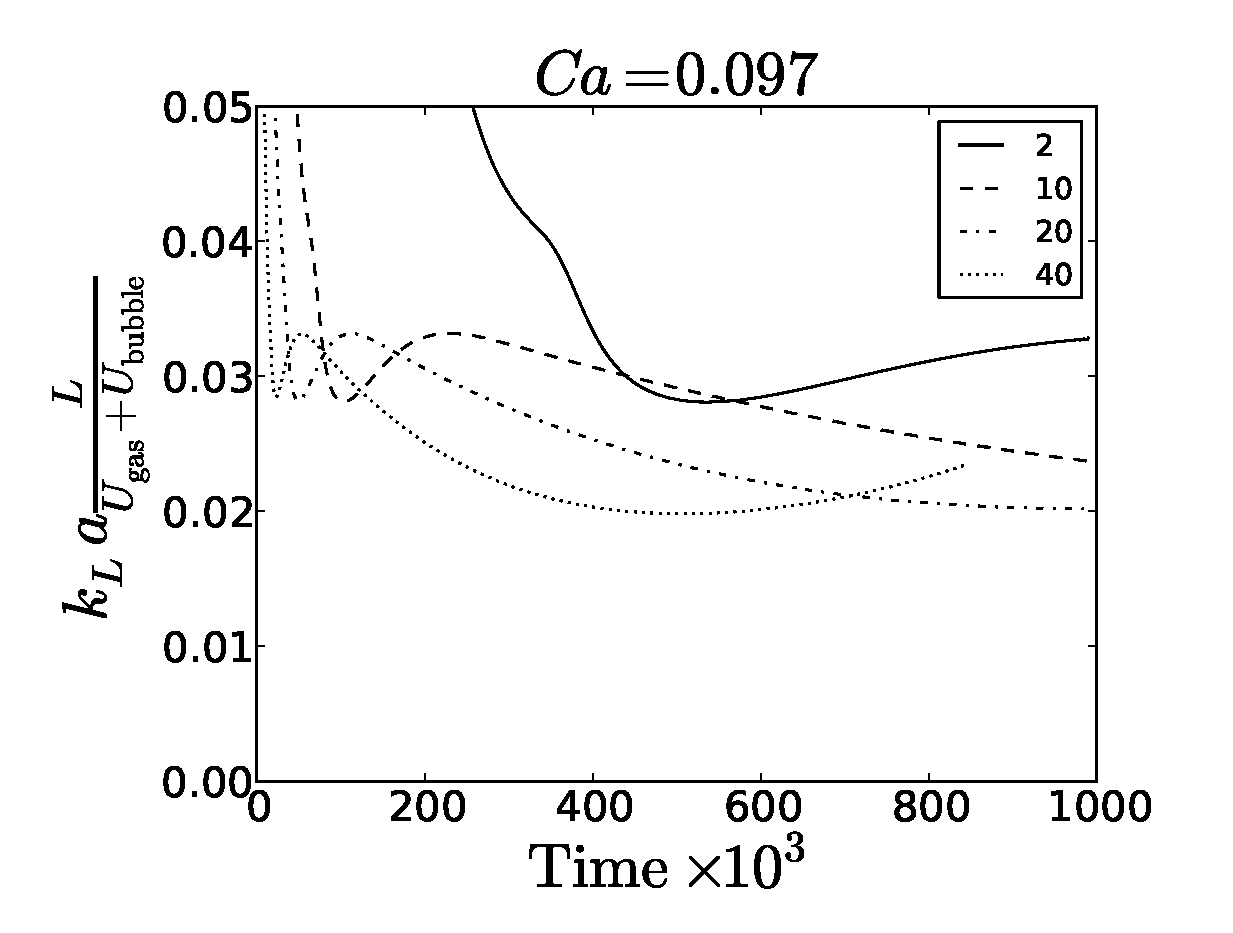
\includegraphics[width=0.5\textwidth]{Figures/sym_aver_moving_window_ca0097.eps}\\
%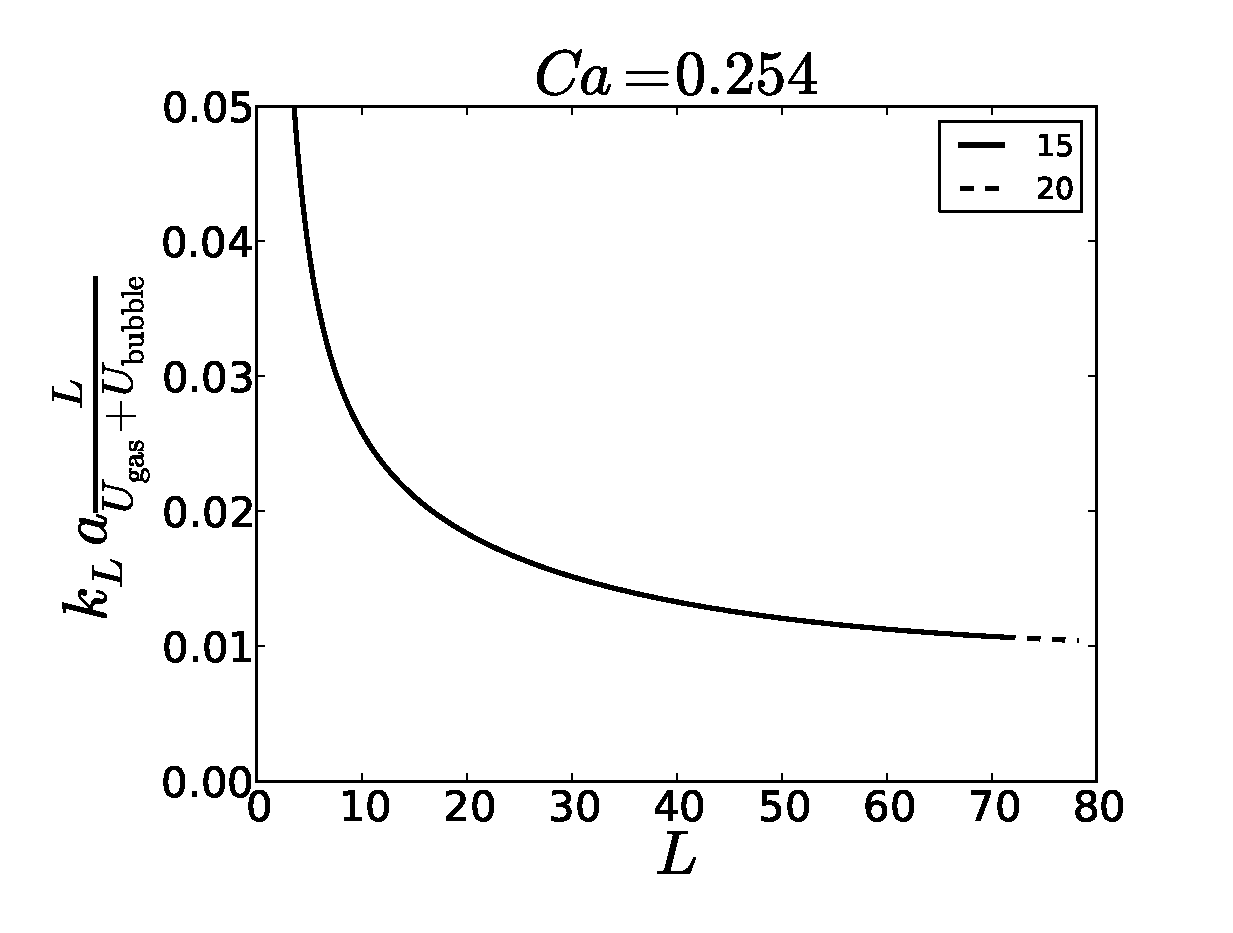
\includegraphics[width=0.5\textwidth]{Figures/sym_aver_conc_scale_ca0254.eps}
%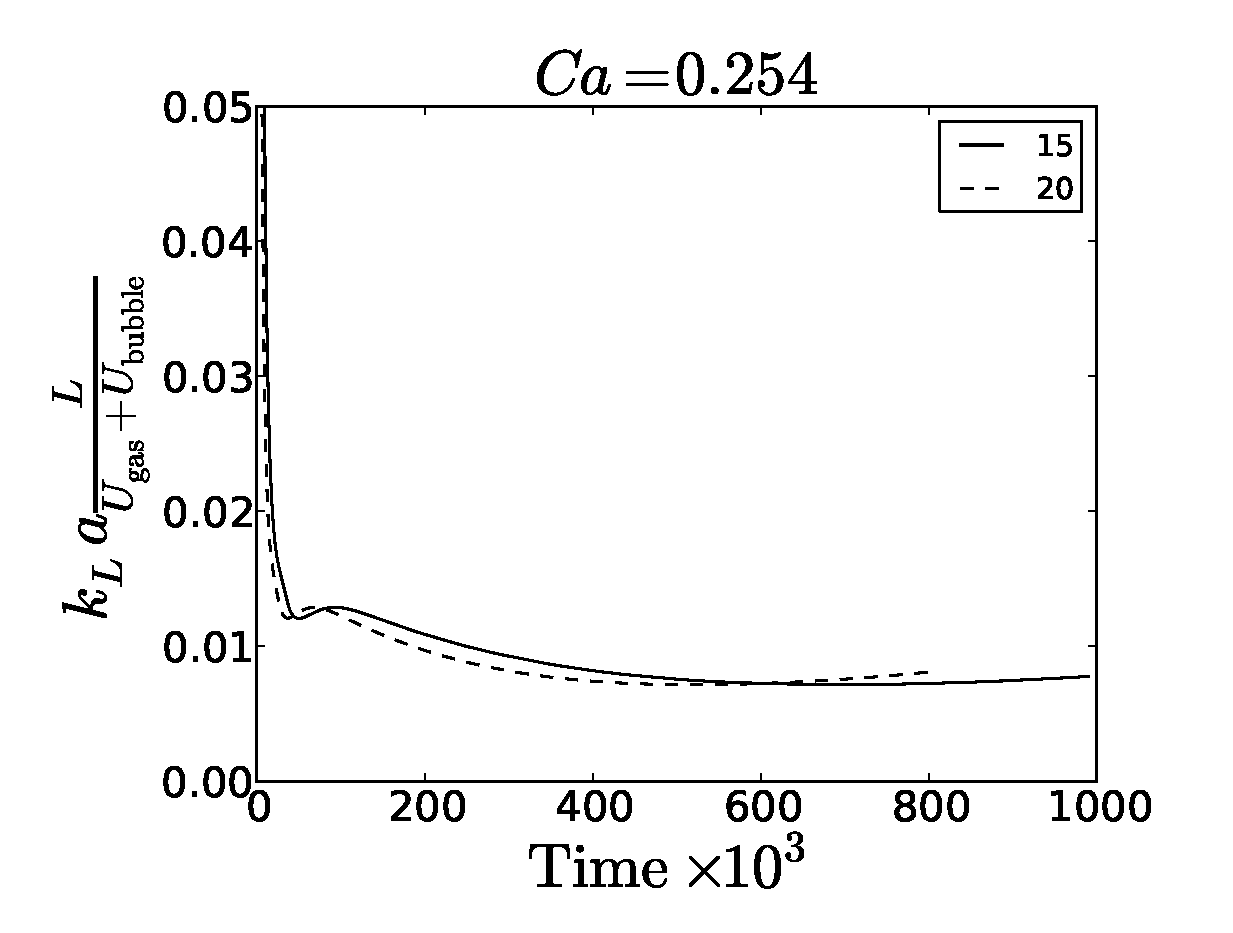
\includegraphics[width=0.5\textwidth]{Figures/sym_aver_moving_window_ca0254.eps}\\
%\caption{Symmetric boundary conditions. \label{fig:open:boundary:sym}}
%\end{figure}

\subsection{Performing a number of cell units simulations}
One needs to examine a few units simulations to obtain a proper volumetric
mass transfer coefficient. This section studies the quantity of the unit cells on the volumetric
mass transfer coefficient to be independent of the number of unit cells. We chose two different
velocity patterns (see Fig. \ref{fig:streamlines:tweaked:velocity} for $Ca=0.097$ and $Ca=1.04$) to
perform a few number of cells simulations. For $Ca=0.097$ we performed simulations with
$4$,$6$,$8$,$10$ number of cells, for $Ca=1.040$ - $4$,$6$,$8$ cells to be examined. However,
simulations with $10$ unit cells domain length produce the same results as $8$ unit cells.
Thus, it won't be covered here, especially as it requires extensive computational resources (grid is
$30000\times 200$). 

As it was discussed in the previous section we want to keep
velocity around $0.05-0.1$ to from . The number of steps for mass to cross whole domain is
limited from above by $1.5 \frac{\lunit}{\ububble}$, which takes into the account the bulk
velocity. If $\ububble$ is taken as $0.05$ then for
the domain size $\lunit=3000$ one can obtain the following number of iteration for mass transfer to
cross the unit cell $1.5 \frac{3000}{0.05}=90000$. Therefore, $10^{6}$ time iterations are enough
for system consisting of $10$ cell units to be stabilized. For more accurate estimations depending
on the Peclet number one can refer to Section \ref{section:keeping:peclet}.

\subsection{$Ca=0.097$ results}
To understand the process happening in unit cells one need to keep a track of a few
characteristics. We chose following representative characteristics: the average concentration in
the unit cell with time, the concentration difference between adjacent unit cells. The latter is
the interesting characteristics which shows how well slug liquid is mixed (to be shown later). The
argument behind this characteristic is that if the following situation is fulfilled: the continuity
equation is satisfied then the concentration along the coordinate changes according to Eq.
\ref{main:mass:transfer:expression}:
\beq
C(x)= \cstar \Bigl(1-\exp\bigl(-\vol \frac{x}{\uliq+\ugas} \bigr)\Bigr)
\feq
%After the transition to the reference frame moving with the velocity $\ububble$, one will have the
%same continuous picture but the concentration dependency will change since velocity is changed as
%well:
%\beq
%C(x)= \cstar \Bigl(1-\exp\bigl(-\vol \frac{x}{\uliq+\ugas-\ububble} \bigr)\Bigr),
%\feq
%Thus, the volumetric mass transfer coefficient for two concentrations which are located at the
%distance $\lunit$ can be found as:
%\beqal
%&\vol \frac{\lunit}{\uliq+\ugas-\ububble}=\ln\Bigl(\frac{\cstar-C_1}{\cstar-C_2}\Bigr)\\
%&\vol
%\frac{\lunit}{\uliq+\ugas}=\frac{\uliq+\ugas-\ububble}{\uliq+\ugas}\ln\Bigl(\frac{\cstar-C_1}{
%\cstar-C_2}\Bigr)
%\feqal
%Parameters $\frac{\uliq+\ugas-\ububble}{\uliq+\ugas}$ were calculated and for representative
%Capillary numbers equal to $0.11,0.04,-0.02,-0.06,-0.10$.
In the case of present simulations the situation is different as the reference frame is moving with
the bubble. Thus, the correlation between adjacent cells as follows:
\beqal
\label{volumetric:between:adjacent:cells}
&C_1=C(x)=C^* \Bigl(1-e^{-\vol \frac{x}{\ugas+\uliq-\ububble}}\Bigr)\\
&C_2=C(x+L)=C^* \Bigl(1-e^{-\vol \frac{x+L}{\ugas+\uliq-\ububble}}\Bigr)\\
&k_L\frac{L}{\ugas+\uliq-\ububble}=\frac{C^*-C_1}{C^{*}-C_2}\\
&k_L\frac{L}{U}=\frac{C^*-C_1}{C^*-C_2},
\feqal
where $U=\ugas+\uliq-\ububble$. We will see later that this characteristic is really important to
see whether the liquid slug is mixed. Fig. \ref{fig:unit:4} shows one of the examples for velocity
scale $20$ and  $4$ unit numbers (all
scales produce the same results) for the volumetric mass transfer coefficient $k_L \frac{L}{U}$
(different from $\volnondim$) based on difference
between two adjacent cells concentration averages. One can see that this number is changed from
segment to segment. The same dependencies can be found for
$6$ and $8$ unit cells simulations but we do not present them here.

However, if one wants to examine how the average concentration changes in time according to Eq.
\ref{theor:continuous:mass:transfer} for different unit cells then one will see interesting
thing for the volumetric mass transfer correlation, see Fig. \ref{fig:moving:average:ca0097}:
\beq
\label{moving:average}
\vol\frac{\lunit}{\ugas+\uliq}=\frac{\lunit}{\ububble (t_2
-t_1)}\ln\Bigl(\frac{C^*-C_1}{C^*-C_2}\Bigr)
\feq
\begin{figure}[htb!]
%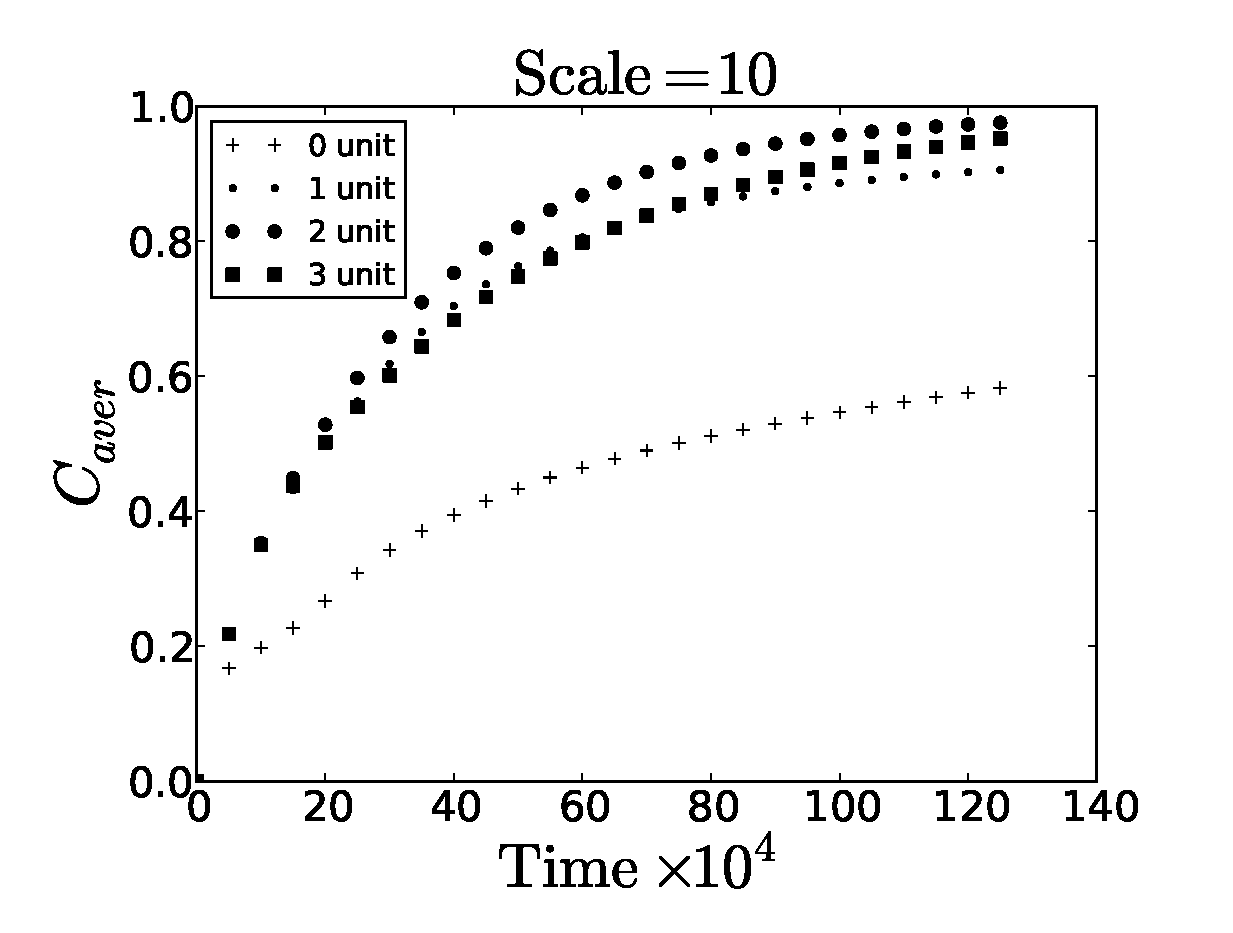
\includegraphics[width=0.5\textwidth]{Figures/aver_units4scale10.eps}\hfill
%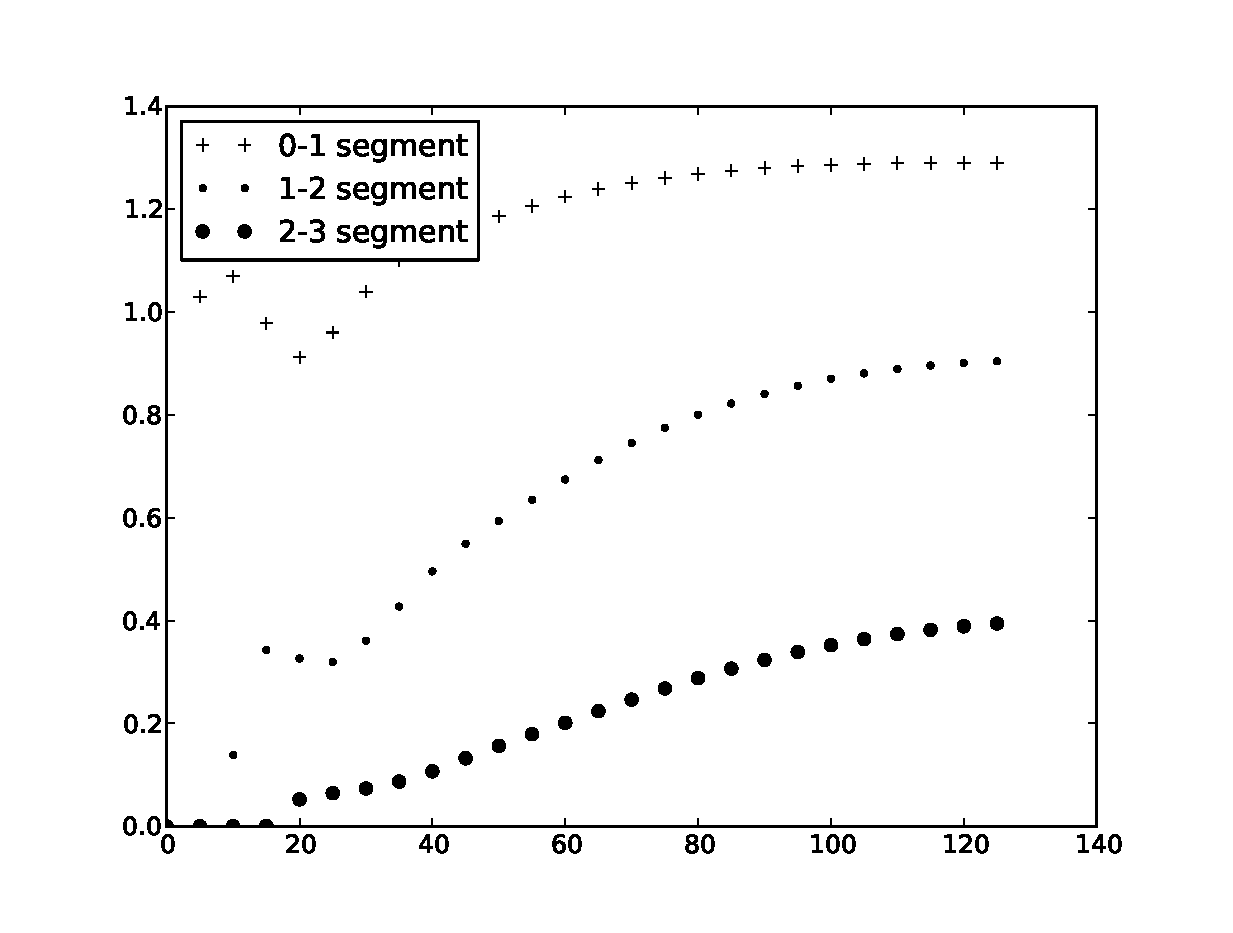
\includegraphics[width=0.5\textwidth]{Figures/coeff_units4scale10.eps}\\
%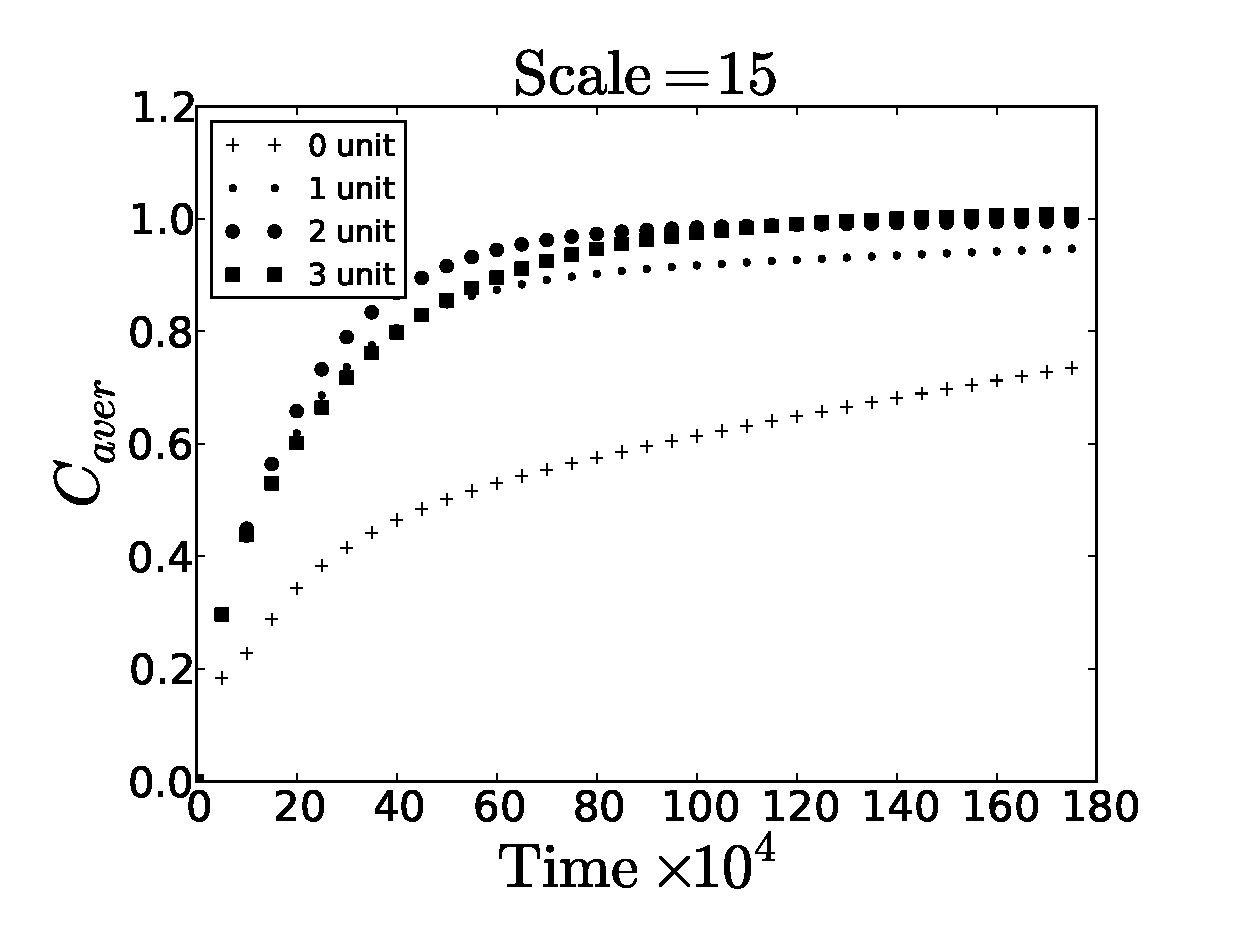
\includegraphics[width=0.5\textwidth]{Figures/aver_units4scale15.eps}\hfill
%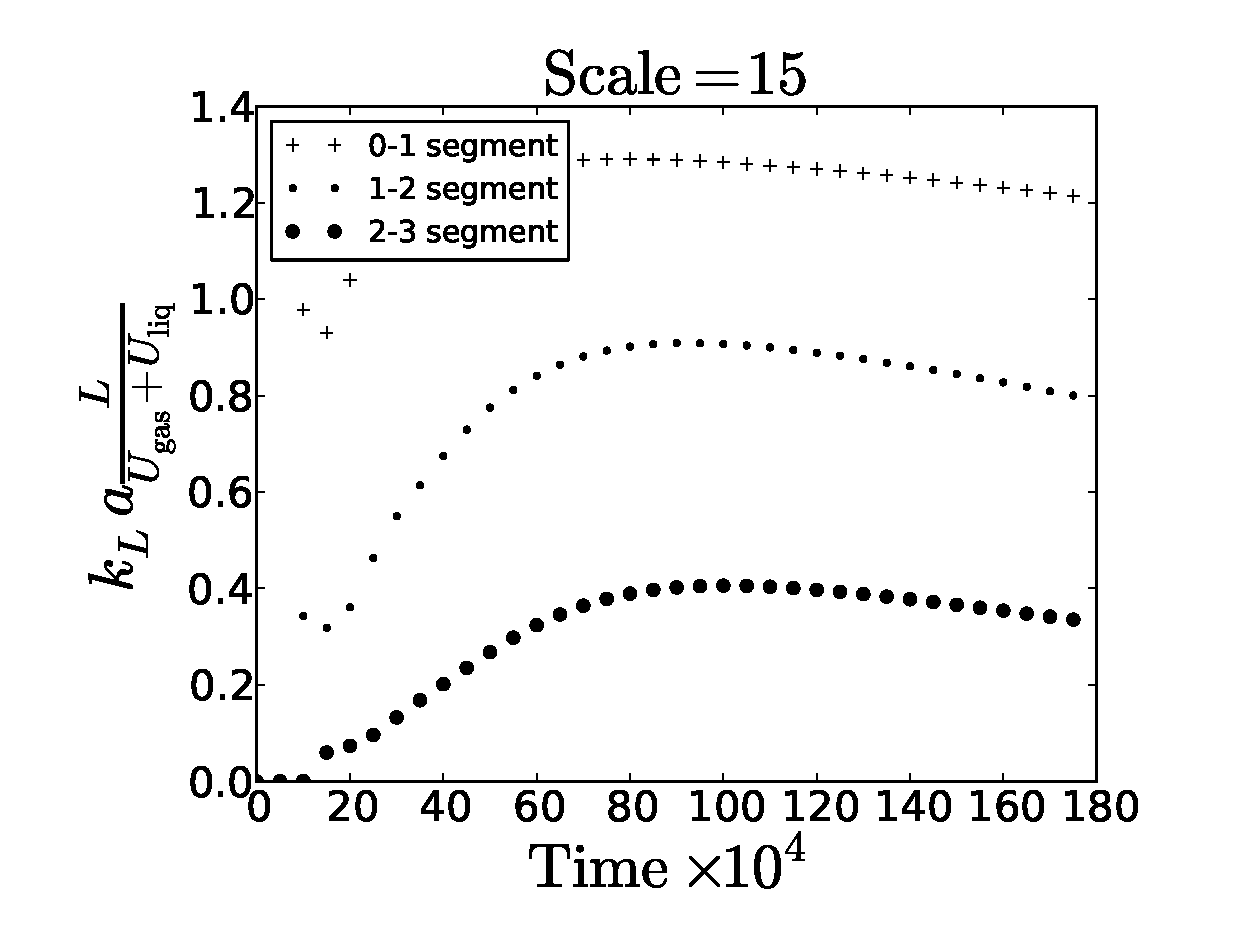
\includegraphics[width=0.5\textwidth]{Figures/coeff_units4scale15.eps}\\
\includegraphics[width=0.5\textwidth]{Figures/aver_units4scale20.eps}\hfill
\includegraphics[width=0.5\textwidth]{Figures/coeff_units4scale20.eps}\\
\caption{Average concentrations (left) and volumetric coefficients (right) $\vol \frac{L}{U}$ (
different from $\volnondim$) for $4$ units cells. The volumetric
mass transfer coefficient is calculated based on the difference between averages for different unit
cells. One can see that the numbers for the volumetric mass transfer coefficient are different for
different unit cells. This is the indication that the liquid slug is mixed and the spatial location
does not easily transfers to time domain. 
\label{fig:unit:4}}
\end{figure}
\begin{figure}[htb!]
\includegraphics[width=0.5\textwidth]{Figures/aver_moving_window4scale10.eps}
\includegraphics[width=0.5\textwidth]{Figures/aver_moving_window6scale10.eps}\\
\includegraphics[width=0.5\textwidth]{Figures/aver_moving_window8scale10.eps}
\caption{The non-dimensional volumetric mass transfer coefficient defined in Eq.
\ref{moving:average} for $4$ (top left),$6$ (top right),$8$ cell units (bottom). Only scale
$10$ is presented since all other simulations produce the same results. One can see that $4$ unit
cells is not enough to avoid the influence of boundaries. However, the results for $6$ and $8$
unit cells are consistent and show that beginning from third unit cell the results and ending with
prelast cell results are consistent with periodic boundary simulations and
\citet{vanbaten-circular} formulations.
\label{fig:moving:average:ca0097}}
\end{figure}

\subsection{$Ca=1.040$ results}
The same correlations were examined for the different velocity pattern $Ca=1.040$ and initial
velocity $\ububble=0.055$ and initial diffusion $D=0.0008375$. A few unit cells simulation for
this
capillary number are unstable. To improve stability we changed original Peclet number by increasing
diffusion to reveal all the correlations. The results for unit cells are the same as for $Ca=0.097$:
at least $6$ unit cells are required to be simulated to avoid the influence of boundaries. Thus,
only $6$ unit cells results are presented in Fig. \ref{fig:6:units:ca1040}. As well the volumetric
mass transfer coefficient, Eq. \ref{volumetric:between:adjacent:cells}, is shown in Fig.
\ref{fig:6:units:ca1040}. One can see that the average volume concentration, as well the volumetric
mass transfer coefficients, come to the constant and are not increasing with time. Thus, all the
mass generated with medium is transfered through the boundaries. This is the indication that the
liquid slug is not mixed. Thus, the volumetric mass transfer coefficient $\volnondim$ can be
calculated according to the definition, Eq. \ref{eq:main:definition}:
\beq
\label{inlet:outlet:spatial:location}
\vol = \frac{\dot{m}}{V \Delta C},
\feq 
where $V$ is the unit cell volume, $\Delta C$ is the concentration difference between the bubble
surface concentration $\cstar$ and the average medium concentration $C_{aver}$. Note that in this
case one can calculate the mass generation as:
\beq
\dot{m}=(\coutlet-\cinlet)\uoutlet,
\feq
where $\coutlet$ and $\cinlet$ are taken for the current unit. Fig. \ref{fig:periodic:ca1040}
(bottom) shows the volumetric mass transfer coefficient, based on spatial calculations of
inlet/outlet concentrations. One can see that the volumetric mass transfer coefficient is close to
the calculated volumetric mass transfer coefficient using the time averaged approach and periodic
boundaries one unit cells simulations. 
\begin{figure}[htb!]
\includegraphics[width=0.5\textwidth]{Figures/aver_units6scaleu2scaled5.eps}
\includegraphics[width=0.5\textwidth]{Figures/novortex6scaleu2scaled5.eps}\\
\caption{Results for 6 unit cells. The Peclet number equals to $Pe=2644$.
One can see that average concentrations reach certain number and stay.
That means whatever was
generated by medium is transfered through the outlet
boundary. One can see that the volumetric mass transfer coefficient based
on the difference between unit cells averages, Eq. \ref{volumetric:between:adjacent:cells}, is
constant for internal
unit cells. This is the indication that the tracer in the slug is not
mixed and the volumetric mass transfer coefficient, $\volnondim$, can be
calculated using the spatial approach, see Fig.
\ref{fig:periodic:ca1040}.\label{fig:6:units:ca1040}}
\end{figure}
The volumetric mass transfer coefficient with periodic boundary simulations for $Pe=2644$ (velocity
scale $2$, diffusion scale $10$) and time dependent, Eq. \ref{theor:continuous:mass:transfer},
average volumetric mass transfer coefficient are presented in Fig. \ref{fig:periodic:ca1040}. Note
that they coincide but are different from calculated coefficients based on spatial location.
Therefore, the time based simulations do not readily convert to spatial based simulations.
\begin{figure}
\includegraphics[width=0.5\textwidth]{Figures/volume_ca_104_scaleu2scaled5.eps}
\includegraphics[width=0.5\textwidth]{Figures/aver_moving_window6scaleu2scaled5.eps}\\
\includegraphics[width=0.5\textwidth]{Figures/flux_moving_window6scaleu2scaled5.eps}\\
\caption{The periodic (top left), time unit cells averaging (top right), and spatial location
(bottom), Eq. \ref{inlet:outlet:spatial:location}, calculated  volumetric mass transfer
coefficients. One can see that they all coincide. However, the periodic boundary conditions based
calculations produce the overestimated volumetric mass transfer
coefficient. \label{fig:periodic:ca1040}}
\end{figure}

\subsection{Experiment comparison}
The goal of this paper is not to compare with the experiment correlations, but give the
procedure to perform numerical simulations in the lattice Boltzmann framework. However, the small
comparison is performed. 
Unfortunately the experiments to the best authors' knowledge measuring the mass flux for infinite
width  bubbles flowing between parallel plates are absent. However, one of interesting
correlations for the mass transfer volumetric coefficient was presented by
\citet{yue-mass} for three-dimensional microchannel geometries:
\beqal
&\vol=\frac{2}{d_h}\Bigl(\frac{D \ububble}{\lbubble+\lslug}\Bigr)^{0.5}
\Bigl(\frac{\lbubble}{\lbubble+\lslug}\Bigr)^{0.3}\\
&\vol \frac{\lunit}{\ugas+\uliq}=2\frac{\lunit}{d_h} \Bigl(\frac{D 
}{\lunit (\ububble+\ugas)} \frac{\ububble}{\ugas+\uliq}\Bigr)^{0.5}
\Bigl(\frac{\lbubble}{\lbubble+\lslug}\Bigr)^{0.3} \propto Pe^{-\frac{1}{2}}\\
&\vol \frac{\lunit}{\ugas+\uliq}=2\frac{\lunit}{d_h} \Bigl(\frac{D 
}{\lunit (\ububble+\ugas)} \frac{\ububble}{\ugas+\uliq}\Bigr)^{0.5}
\Bigl(\frac{\lbubble}{\lbubble+\lslug}\Bigr)^{0.3} \propto Pe^{-\frac{1}{2}}
\feqal
One can see that approximately the volumetric mass transfer correlation should be proportional to
$Pe^{-0.5}$. Fig. \ref{fig:volume:mass:coefficient} shows a comparison between corelation by
\citet{yue-mass} and the current simulations coefficients presented in Table
\ref{table:steady:state:average}. The coefficients are not far from each other, given the difference
between two-dimensional and three-dimensional cases. The fitting procedure showed that the power of
the Peclet number $Pe$ is $-0.50038$ which is close to $-0.5$. 
\begin{figure}[htb!]
\includegraphics[width=\textwidth]{Figures/correlations_comparison.eps}
\caption{Comparison between correlation by \citet{yue-mass} and mass transfer coefficient based
on periodic boundary conditions. The fitting curve is proportional to $Pe^{-0.5}$ which corresponds
to the correlation by \citet{yue-mass}.\label{fig:volume:mass:coefficient}}
\end{figure}

\section{Conclusion}
This work examines a way to calculate the volumetric mass transfer coefficient in the framework of
the lattice Boltzmann method. Overall, the recipe is to perform periodic boundary
conditions simulations and calculate the volumetric mass transfer coefficient based on the averaged
domain concentration through any formulation as they produce consistent results. However, the
result is the volumetric mass transfer coefficient will be overestimated using this
approach. Formulation of
\citet{vanbaten-circular} is inconsistent if one takes the inlet/outlet flux averaged concentration
to be characteristic concentration. A few unit cells simulations are harder to perform, but they
have indicator of how well the liquid slug is mixed. As well, for velocity patterns for $Ca\geq
0.7$ simulations with a few unit cells allow to calculate the volumetric mass transfer
coefficient based on the spatial location, not time averaged values used in all other
approaches. Finally, a sample of results was
compared with the experimental correlation of \citet{yue-mass}. 
\appendix
\section{Analytical solution for parabolic profile with zero velocity gradient at $0$}
\label{appendix:zero:gradient}
The problem is defined in terms of PDE as follows: 
\beq
\label{diffusion:zero:gradient:start}
\begin{aligned}
&\frac{\partial C}{\partial x} U(y)=D\frac{\partial^2 C}{\partial y^2}\\
&C(0,y)=C_0,\, C(x,0)=\cstar,\, \frac{\partial C}{\partial y }(x,\delta)=0\\
&U(y)=U_0 \Bigl(\frac{y}{\delta}\Bigr)^2
\end{aligned}
\feq
The non-dimensional parameters are introduced:
\beq
\begin{aligned}
&\frac{\partial C}{\partial \frac{x}{H}} \frac{U_0}{H}
\Bigl(\frac{y}{H}\Bigr)^2=\frac{D}{H^2}\frac{\partial^2 C}{\partial \frac{y^2}{H^2}}\\
&C(0,y)=C_0,\, C(x,0)=\cstar,\, \frac{\partial C}{\partial y }(x,H)=0\\
\end{aligned}
\feq
After a change of variables:
\beq
\begin{aligned}
&\zeta=\frac{x}{H} \frac{D}{U_0 H}=\frac{1}{Pe}\frac{x}{H}\\
&\xi=\frac{y}{H},
\end{aligned}
\feq 
Eq. \ref{diffusion:zero:gradient:start} with boundary conditions becomes as follows:
\beq
\label{diffusion:zero:gradient:middle}
\begin{aligned}
&\frac{\partial C}{\partial \zeta}\xi^2=\frac{\partial^2 C}{\partial \xi^2}\\
&C(0,\xi)=C_0\\
&C(\zeta,0)=\cstar\\
&\frac{\partial C}{\partial \xi}(\zeta,1)=0\\
\end{aligned}
\feq 
Still Eq. \ref{diffusion:zero:gradient:middle} cannot be solved with the separation of variables as it requires homogenous
boundary conditions. Thus, let us introduce the new variable, $\Theta=C-\cstar$, which makes the system to be with homogenous boundary conditions:
\beq
\begin{aligned}
&\frac{\partial \Theta}{\partial \zeta}=\frac{1}{\xi^2}\frac{\partial^2 \Theta}{\partial \xi^2}\\
&\Theta(0,\xi)=C_0-\cstar \\
&\Theta(\zeta,0)=0,\, \partial_{\xi}\Theta(\zeta,1)=0\\
\end{aligned}
\feq 
This equation can be solved by separation of variables if the solutions is represented as the
multiplication of two functions $\Theta(\zeta,\xi)=X(\zeta)Y(\xi)$:
\beq
\begin{aligned}
&\frac{\mathrm{d} X(\zeta)}{\mathrm{d} \zeta}Y(\xi)=\frac{X(\zeta)}{\xi^2}\frac{\mathrm{d^2}
Y(\xi)}{\mathrm{d}\xi^2}\\
&\frac{1}{X(\zeta)}\frac{\mathrm{d} X(\zeta)}{\mathrm{d} \zeta}=\frac{1}{\xi^{2} Y(\xi)}
\frac{\mathrm{d^2} Y(\xi)}{\mathrm{d}\xi^2}
\end{aligned}
\feq
The left and right parts depend on different variables. Therefore to be equal to each other both
parts shall equal to constant, say $-m^4$. Thus, the separation of the variables leads to two ODEs:
\begin{equation*}
\begin{aligned}
&\frac{\mathrm{d}X(\zeta)}{\mathrm{d}\zeta}=-m^4 X(\zeta)\\
&\frac{\mathrm{d^2}Y(\xi)}{\mathrm{d}\xi^2}+m^4 \xi^2 Y(\xi)=0\\ 
\end{aligned}
\end{equation*}
The solution of the first equation is the exponential function:
\beq
X(\zeta)=\exp(-m^4 \zeta)\\
\feq
The solutions of the second equation are two hypergeometric function which can be expressed through
the Bessel functions \cite{abramowitz}:
\beq
\begin{aligned}
&Y_1=\sqrt{\xi}J_{\frac{1}{4}}\Bigl(\frac{m^2 \xi^2}{2}\Bigr)\\
&Y_2=\sqrt{\xi}J_{-\frac{1}{4}}\Bigl(\frac{m^2 \xi^2}{2}\Bigr)\\
&Y'_1=m^2 \xi^{3/2} J_{-\frac{3}{4}}\Bigl(\frac{m^2 \xi^2}{2}\Bigr)\\
&Y'_2=m^2 \xi^{3/2} J_{\frac{3}{4}}\Bigl(\frac{m^2 \xi^2}{2}\Bigr)\\
\end{aligned}
\feq
The solution is the summation of two functions:
\begin{equation*}
Y(x)=C_1 Y_1(x)+C_2 Y_2(x). 
\end{equation*}
One can find coefficients from the boundary conditions:
\beq
\begin{aligned}
&Y(0)=0=C_1 Y_1(0)+C_2 Y_2(0)\\
&Y_1(0)=0,\,Y_2(0)=\frac{\sqrt{2}}{\sqrt{m} \Gamma(3/4)}\, C_2=0\\
&Y'(1)=0=C_1 Y'_1(1)+C_2 Y'_2(1)=C_1 Y'_1(1)\\
&J_{-\frac{3}{4}}\Bigl(\frac{m^2}{2}\Bigr)=0
\end{aligned}
\feq
Therefore one needs to find zeros of $J_{-\frac{3}{4}}\Bigl(\frac{m^2}{2}\Bigr)$. To give some
numerical values:
$m_1=1.454997085$, $m_2=2.927133004$, $m_3=3.857578101$, $m_4=4.601777732$, $m_5=5.240824067$.
Therefore, the solution in a general form is represented as:
\beq
\Theta(\zeta,\xi)=\sum_m{C_m \sqrt{\xi} J_{\frac{1}{4}}\Bigl(\frac{m^2
\xi^2}{2}\Bigr)\exp(-m^4 \zeta)}
\feq
To find unknown coefficients $C_m$ one needs to substitute the expression above to the initial
condition:
\beq
\Theta(0,\xi)=C_0-\cstar=\sum_m{C_m \sqrt{\xi}J_{\frac{1}{4}}\Bigl(\frac{m^2
\xi^2}{2}\Bigr)}\\
\feq
Using the Stourm-Liouville theorem one can multiply by $\xi^{5/2}
J_{\frac{1}{4}}\Bigl(\frac{m^2 \xi^2}{2}\Bigr)$ and integrate left and right parts of the equation:
\beq
\begin{aligned}
&\bigl(C_0-\cstar\bigr) \int_{\xi=0}^{1}{\xi^{5/2} J_{\frac{1}{4}}\Bigl(\frac{m^2
\xi^2}{2}\Bigr)\mathrm{d}\xi}=C_m\int_{\xi=0}^{1}{\xi^3 J_{\frac{1}{4}}^2\Bigl(\frac{m^2
\xi^2}{2}\Bigr)\mathrm{d}\xi}\\
&C_m = (C_0-\cstar ) \frac{\int_{\xi=0}^{1}{\xi^{5/2} J_{\frac{1}{4}}\Bigl(\frac{m^2
\xi^2}{2}\Bigr)\mathrm{d}\xi}}{\int_{\xi=0}^{1}{\xi^3 J_{\frac{1}{4}}^2\Bigl(\frac{m^2
\xi^2}{2}\Bigr)\mathrm{d}\xi}}
\end{aligned}
\feq
Therefore, the overall solution is specified as:
\beq
\begin{aligned}
&C(x,y)=\cstar+\sum_{m}{C_m
\sqrt{\frac{y}{H}}J_{\frac{1}{4}}\Bigl(\frac{m^2}{2}\frac{y^2}{H^2}\Bigr)\exp\Bigl(-\frac{m^4}{Pe}
\frac { x }{H}\Bigr)}\\
&C_m = (C_0-\cstar) \frac{\int_{\xi=0}^{1}{\xi^{5/2} J_{\frac{1}{4}}\Bigl(\frac{m^2
\xi^2}{2}\Bigr)\mathrm{d}\xi}}{\int_{\xi=0}^{1}{\xi^3 J_{\frac{1}{4}}^2\Bigl(\frac{m^2
\xi^2}{2}\Bigr)\mathrm{d}\xi}}
\end{aligned}
\feq
For the sake of completeness, we list $5$ first coefficients for a case $C_0=0$ and $\cstar=1$:
$C_1=-1.5217$, $C_2=-0.4933$, $C_3=-0.3243$, $C_4=-0.2486$, $C_5=-0.2044$. 
\subsection{The Poiseuille parabolic profile}
\label{appendix:poiseuille}
Close to the previous example but with a different velocity profile, the benchmark can be
formulated through the following PDE:
\beq
\begin{aligned}
&\frac{\partial C}{\partial x} U(y)=D\frac{\partial^2 C}{\partial y^2}\\
&C(0,y)=0,\, C(x,\pm \delta)=\cstar,\, \frac{\partial C}{\partial y }(x,0)=0\\
&U(y)=U_0 \Bigl(1-\bigl(\frac{y}{\delta}\bigr)^2\Bigr)
\end{aligned}
\feq
The same procedure can be done as in the previous case to redefine variables. After substitution
the following equation can be obtained:
\beq
\begin{aligned}
&\frac{\partial \Theta}{\partial \zeta}(1-\xi^2)=\frac{\partial^2 C}{\partial \xi^2}\\
&\Theta(\zeta,\xi)=C-\cstar\,\Theta(0,\xi)=-\cstar\,\Theta(0,\pm 1)=0
\end{aligned}
\feq
After separation of variables, $\Theta(\zeta,\xi)=X(\zeta)Y(\xi)$ one can come up with two
equations:
\beq
\label{fourier:separation:variables:parabolic}
\begin{aligned}
&\frac{\mathrm{d}X(\zeta)}{\mathrm{d}\zeta}+m^4 X(\zeta)=0\\
&\frac{\mathrm{d^2}Y(\xi)}{\mathrm{d}\xi^2}+m^4 (1-\xi^2) Y(\xi)=0
\end{aligned}
\feq
The first equation has a solution:
\beq
X(\zeta)=\exp(-m^4 \zeta)
\feq
The second equation can be simplified after substitution $\bar{\xi}=m \sqrt{2} \xi$ to the standard
equation:
\beq
Y''-\Bigl(\frac{1}{4}\xi^2+a\Bigr)Y=0.
\feq
The equation above has two solutions via parabolic cylinder functions or through the confluent
hypergeometric function \cite{abramowitz}:
\beq
\begin{aligned}
&Y_1=e^{-x^2/4} {_1F_1}\Bigl(\frac{a}{2}+\frac{1}{4},\frac{1}{2},\frac{x^2}{2}\Bigr)\\
&Y_2=e^{-x^2/4} {_1F_1}\Bigl(\frac{a}{2}+\frac{3}{4},\frac{3}{2},\frac{x^2}{2}\Bigr)\\
\end{aligned}
\feq 
Taking symmetry conditions in the consideration by leaving only even solution, Eq.
\ref{fourier:separation:variables:parabolic} has a solution as:
\beq
Y_m=C_m e^{-m^2 x^2/2} {_1F_1}\Bigl(-\frac{m^2}{4}+\frac{1}{4},\frac{1}{2},m^2 x^2\Bigr) 
\feq
To satisfy boundary condition we need to find zeros of the hypergeometric function, i.e.
${_1F_1}\Bigl(-\frac{m^2}{4}+\frac{1}{4},\frac{1}{2},m^2 \Bigr)=0$. First ten eigenvalues can be
found using numerical methods, as $1.2967$, $2.3811$,$3.1093$,$3.6969$,$4.2032$,$4.6548$,$5.0662$,
$5.4467$, $5.8023$,$6.1373$. One needs to satisfy one more condition to obtain coefficients $C_m$:
\beq
-\cstar=\sum_m{C_m e^{-m^2 x^2/2} {_1F_1}\Bigl(-\frac{m^2}{4}+\frac{1}{4},\frac{1}{2},m^2
x^2\Bigr)} 
\feq
One can multiply both parts on $(1-x^2){_1F_1}\Bigl(-\frac{m^2}{4}+\frac{1}{4},\frac{1}{2},m^2
x^2\Bigr)$ and through orthoganality (Stourm-Liouiville theorem) obtain coefficients:
\beq
\label{coeff:series:parabolic:profile}
C_m=-\cstar \frac{\int_{x=0}^{1}{(1-x^2)e^{-m^2 x^2/2}
{_1F_1}\Bigl(-\frac{m^2}{4}+\frac{1}{4},\frac{1}{2},m^2
x^2\Bigr)\mathrm{d}x}}{\int_{x=0}^{1}{(1-x^2)e^{-m^2 x^2/2}
{_1F_1}\Bigl(-\frac{m^2}{4}+\frac{1}{4},\frac{1}{2},m^2
x^2\Bigr)^2\mathrm{d}x}}
\feq
Therefore a whole solution can be written as:
\begin{equation}
C=\cstar-\cstar \sum_{m=0}{C_m e^{-m^4 \frac{x}{\delta}\frac{1}{Pe}} e^{-m^2
y^2/(2\delta^2)}{_1F_1}\Bigl(-\frac{m^2}{4}+\frac{1}{4},\frac{1}{2},m^2 \frac{y^2}{\delta^2}\Bigr)},
\end{equation}
where coefficients $C_m$ are taken from Eq. \ref{coeff:series:parabolic:profile}. For the case
$\cstar$, first ten coefficients equal to  $1.2008$, $-0.2991$, $0.1608$, $-0.1074$, $0.0796$,
$-0.0627$, $0.0515$, $-0.0435$, $0.0375$, $-0.0329$.

\section{Free surface boundary conditions}
\label{appendix-free-surface}
There are a few implementations of free boundary conditions \cite{ginzburg-free,verberg-free}.
However, we developed the easy solver to impose the free surface boundary conditions at the
complicated surface of the bubble. The reason is to impose the symmetric boundary conditions.
Because the boundary is the staircase approximation, one can find the normal to the boundary which
is always located by the angle of multiple of $45$ degrees, see Fig. \ref{fig:free:surface}. This
can be done automatically by the` simple coding. Imposing the
symmetric boundary conditions requires $U_{n,F}$=$U_{n,B}$ and $U_{\tau,F}=U_{\tau,B}$. We can copy
populations in the certain order to do it, for example $f_{B,i}=f_{F,\bar{i}}$, where $c_i$ and
$c_{\bar{i}}$ are complementary directions, where $c_{i,n}=-c_{\bar{i},n}$ and
$c_{i,\tau}=c_{\bar{i},\tau}$, where $c_{i,n}=(\bm{c_i} \cdot \bm{n})\bm{n}$ and
$c_{i,\tau}=\bm{c_i}-(\bm{c_i}\cdot \bm{n})\bm{n}$.  

\begin{figure}
\includegraphics[width=0.5\textwidth]{Figures/free_surface.eps}
\caption{Free-surface boundary condition represented in the lattice Boltzmann. By crosses we outline
boundary nodes, by circle the fluid node is outlined. Populations at the corner boundary nodes are
essentially the population of the fluid node, but in the certain order. \label{fig:free:surface}}
\end{figure}
\bibliographystyle{unsrtnat}
\bibliography{paper}
\end{document}

